% !TeX spellcheck = pl_PL
%%%%%%%%%%%%%%%%%%%%%%%%%%%%%%%%%%%%%%%%%%%
%                                        %
% Szablon pracy dyplomowej magisterskiej %
% zgodny  z aktualnymi  przepisami  SZJK %
%                                        %
%%%%%%%%%%%%%%%%%%%%%%%%%%%%%%%%%%%%%%%%%%
%                                        %
%  (c) Krzysztof Simiński, 2018-2023     %
%                                        %
%%%%%%%%%%%%%%%%%%%%%%%%%%%%%%%%%%%%%%%%%%
%                                        %
% Najnowsza wersja szablonów jest        %
% podstępna pod adresem                  %
% github.com/ksiminski/polsl-aei-theses  %
%                                        %
%%%%%%%%%%%%%%%%%%%%%%%%%%%%%%%%%%%%%%%%%%
%
%
% Projekt LaTeXowy zapewnia odpowiednie formatowanie pracy,
% zgodnie z wymaganiami Systemu zapewniania jakości kształcenia.
% Proszę nie zmieniać ustawień formatowania (np. fontu,
% marginesów, wytłuszczeń, kursywy itd. ).
%
% Projekt można kompilować na kilka sposobów.
%
% 1. kompilacja pdfLaTeX
%
% pdflatex main
% bibtex   main
% pdflatex main
% pdflatex main
%
%
% 2. kompilacja XeLaTeX
%
% Kompilatacja przy użyciu XeLaTeXa różni się tym, że na stronie
% tytułowej używany jest font Calibri. Wymaga to jego uprzedniego
% zainstalowania.
%
% xelatex main
% bibtex  main
% xelatex main
% xelatex main
%
%
%%%%%%%%%%%%%%%%%%%%%%%%%%%%%%%%%%%%%%%%%%%%%%%%%%%%%
% W przypadku pytań, uwag, proszę pisać na adres:   %
%      krzysztof.siminski(małpa)polsl.pl            %
%%%%%%%%%%%%%%%%%%%%%%%%%%%%%%%%%%%%%%%%%%%%%%%%%%%%%
%
% Chcemy ulepszać szablony LaTeXowe prac dyplomowych.
% Wypełniając ankietę spod poniższego adresu pomogą
% Państwo nam to zrobić. Ankieta jest całkowicie
% anonimowa. Dziękujemy!


% https://docs.google.com/forms/d/e/1FAIpQLScyllVxNKzKFHfILDfdbwC-jvT8YL0RSTFs-s27UGw9CKn-fQ/viewform?usp=sf_link
%
%%%%%%%%%%%%%%%%%%%%%%%%%%%%%%%%%%%%%%%%%%%%%%%%%%%%%%%%%%%%%%%%%%%%%%%%%

%%%%%%%%%%%%%%%%%%%%%%%%%%%%%%%%%%%%%%%%%%%%%%%
%                                             %
% PERSONALIZACJA PRACY – DANE PRACY           %
%                                             %
%%%%%%%%%%%%%%%%%%%%%%%%%%%%%%%%%%%%%%%%%%%%%%%

% Proszę wpisać swoje dane w poniższych definicjach.

% TODO
% dane autora
\newcommand{\FirstNameAuthor}{Piotr}
\newcommand{\SurnameAuthor}{Marcol}
\newcommand{\IdAuthor}{300463}   % numer albumu  (bez $\langle$ i $\rangle$)

% drugi autor:
%\newcommand{\FirstNameCoauthor}{Imię}   % Jeżeli jest drugi autor, to tutaj należy podać imię.
%\newcommand{\SurnameCoauthor}{Nazwisko} % Jeżeli jest drugi autor, to tutaj należy podać nazwisko.
%\newcommand{\IdCoauthor}{$\langle$wpisać właściwy$\rangle$}  % numer albumu drugiego autora (bez $\langle$ i $\rangle$)
% Gdy nie ma drugiego autora, należy zostawić poniższe definicje puste, jak poniżej. Gdy jest drugi autor, należy zakomentować te linie.
\newcommand{\FirstNameCoauthor}{} % Jeżeli praca ma tylko jednego autora, to dane drugiego autora zostają puste.
\newcommand{\SurnameCoauthor}{}   % Jeżeli praca ma tylko jednego autora, to dane drugiego autora zostają puste.
\newcommand{\IdCoauthor}{}  % Jeżeli praca ma tylko jednego autora, to dane drugiego autora zostają puste.
%%%%%%%%%%

\newcommand{\Supervisor}{Dr hab. inż., prof. PŚ Michał Maćkowski}     % dane promotora (bez $\langle$ i $\rangle$)
\newcommand{\Title}{System przeznaczony dla osób niewidomych do rozpoznawania dotykanych obiektów 3D}           % tytuł pracy po polsku
\newcommand{\TitleAlt}{A system designed for the blind to recognize touched 3D objects}                     % thesis title in English
\newcommand{\Program}{Informatyka}            % kierunek studiów  (bez $\langle$ i $\rangle$)
\newcommand{\Specialisation}{Oprogramowanie Systemowe}     % specjalność  (bez $\langle$ i $\rangle$)
\newcommand{\Departament}{Systemów Rozproszonych i Urządzeń Informatyki}        % katedra promotora  (bez $\langle$ i $\rangle$)

% Jeżeli został wyznaczony promotor pomocniczy lub opiekun, proszę go/ją wpisać ...
% \newcommand{\Consultant}{$\langle$stopień naukowy imię i nazwisko$\rangle$} % dane promotora pomocniczego, opiekuna (bez $\langle$ i $\rangle$)
% ... w przeciwnym razie proszę zostawić puste miejsce jak poniżej:
\newcommand{\Consultant}{} % brak promotowa pomocniczego / opiekuna

% koniec fragmentu do modyfikacji
%%%%%%%%%%%%%%%%%%%%%%%%%%%%%%%%%%%%%%%%%%


%%%%%%%%%%%%%%%%%%%%%%%%%%%%%%%%%%%%%%%%%%%%%%%
%                                             %
% KONIEC PERSONALIZACJI PRACY                 %
%                                             %
%%%%%%%%%%%%%%%%%%%%%%%%%%%%%%%%%%%%%%%%%%%%%%%

%%%%%%%%%%%%%%%%%%%%%%%%%%%%%%%%%%%%%%%%

\input{config/settings.tex} % Proszę nie modyfikować pliku settings.tex


%%%%%%%%%%%%%%%%%%%%%%%%%%%%%%%%%%%%%%%%%%%%%%%
%                                             %
% MOJE PAKIETY, USTAWIENIA ITD                %
%                                             %
%%%%%%%%%%%%%%%%%%%%%%%%%%%%%%%%%%%%%%%%%%%%%%%

% Tutaj proszę umieszczać swoje pakiety, makra, ustawienia itd.

%%%%%%%%%%%%%%%%%%%%%%%%%%%%%%%%%%%%%%%%%%%%%%%
% Dodatkowe ustawienia typograficzne autora
%%%%%%%%%%%%%%%%%%%%%%%%%%%%%%%%%%%%%%%%%%%%%%%

% % --- Polska typografia: sieroty jednoliterowe ---
% \babelprovide[transforms = oneletter.nobreak]{polish}

% --- Wdowy i sieroty akapitowe ---
\clubpenalty=10000
\widowpenalty=10000
\displaywidowpenalty=10000
\brokenpenalty=10000
\emergencystretch=2em
% \raggedbottom



%%%%%%%%%%%%%%%%%%%%%%%%%%%%%%%%%%%%%%%%%%%%%%%%%%%%%%%%%%%%%%%%%%%%%
% listingi i fragmentu kodu źródłowego 
% pakiet: listings lub minted
% % % % % % % % % % % % % % % % % % % % % % % % % % % % % % % % % % % 

% biblioteka listings
\usepackage{listings}
\lstset{%
    morekeywords={string,exception,std,vector},% słowa kluczowe rozpoznawane przez pakiet listings
    language=C++,% C, Matlab, Python, SQL, TeX, XML, bash, ... – vide https://www.ctan.org/pkg/listings
    commentstyle=\textit,%
    identifierstyle=\textsf,%
    keywordstyle=\sffamily\bfseries, %\texttt, %
    %captionpos=b,%
    tabsize=3,%
    frame=lines,%
    numbers=left,%
    numberstyle=\tiny,%
    numbersep=5pt,%
    breaklines=true,%
    escapeinside={@*}{*@},%
}

% % % % % % % % % % % % % % % % % % % % % % % % % % % % % % % % % % % 
% pakiet minted
% \usepackage{minted}

% pakiet wymaga specjalnego kompilowania:
% pdflatex -shell-escape main.tex
% xelatex  -shell-escape main.tex

\usepackage[chapter]{minted} % [section]
%\usemintedstyle{bw}   % czarno-białe kody 

\setminted % https://ctan.org/pkg/minted
{
    %fontsize=\normalsize,%\footnotesize,
    %captionpos=b,%
    tabsize=3,%
    frame=lines,%
    framesep=2mm,
    numbers=left,%
    numbersep=5pt,%
    breaklines=true,%
    escapeinside=@@,%
}

%%%%%%%%%%%%%%%%%%%%%%%%%%%%%%%%%%%%%%%%%%%%%%%%%%%%%%%%%%%%%%%%%%%%%

% moje polecenia

\usepackage{xcolor}
\usepackage{ifthen}
\usepackage{tabularx}
\usepackage{array}
\usepackage{float}
\usepackage{pdflscape}
\usepackage{caption}
\usepackage{rotating}
\usepackage{makecell}
% \usepackage{showframe} % ! Disable in the final version of the document

% ?: Tabele

\AddToHook{env/table/begin}{%
  \setlength{\tabcolsep}{4pt}%
  \renewcommand{\arraystretch}{1.25}%
}

% ?: Rysunki

\usetikzlibrary{positioning}

% ! comment these lines to disable watermark in the final version of the document

\usepackage{draftwatermark}
\SetWatermarkText{DRAFT}
\SetWatermarkScale{1}

% ! end of section to disable watermark in the final version of the document

\newcommand{\note}[2][]{}

\newcommand{\draft}[2][]{}

% ! Comment next section to disable notes and drafts in the final version of the document

\renewcommand{\note}[2][]{%
    \ifthenelse{\equal{#1}{hide}}%
    {}%
    {{\color{red}{#2}}}%
}

\renewcommand{\draft}[2][]{%
    \ifthenelse{\equal{#1}{hide}}%
    {}%
    {{\color{olive}{#2}}}%
}

% ! end of section to disable notes and drafts in the final version of the document

%%%%%%%%%%%%%%%%%%%%%%%%%%%%%%%%%%%%%%%%%%%%%%%
%                                             %
% KONIEC MOICH USTAWIEŃ                       %
%                                             %
%%%%%%%%%%%%%%%%%%%%%%%%%%%%%%%%%%%%%%%%%%%%%%%

 % Tutaj proszę umieścić swoje pakiety, makra, ustawienia itd.

%%%%%%%%%%%%%%%%%%%%%%%%%%%%%%%%%%%%%%%%


\begin{document}
%\kslistofremarks

\frontmatter
\input{config/titlepage.tex}  % Proszę nie modyfikować pliku titlepage.tex

\cleardoublepage

\rmfamily\normalfont
\pagestyle{empty}


%%% No to zaczynamy pisać pracę :-) %%%%

% TODO
\subsubsection*{Tytuł pracy} 
\Title

\subsubsection*{Streszczenie}  
% (Streszczenie pracy – odpowiednie pole w systemie APD powinno zawierać kopię tego streszczenia.)

Celem niniejszej pracy było opracowanie systemu wspomagającego osoby niewidome i słabowidzące w nauce geometrii przestrzennej poprzez rozpoznawanie fizycznych modeli brył podczas ich eksploracji dotykowej. W ramach pracy zaprojektowano i zaimplementowano prototyp systemu działający w architekturze klient-serwer, wykorzystujący aplikację mobilną do rejestracji obrazu i komunikacji z użytkownikiem oraz część serwerową wykonującą detekcję i analizę obiektów. System umożliwia analizę widocznej powierzchni bryły oraz przekazanie użytkownikowi informacji na jej temat zawartych w bazie wiedzy. Przygotowano własny zbiór danych obejmujący sześć klas brył geometrycznych oraz przeprowadzono eksperymenty dla siedmiu konfiguracji modeli YOLO26 badając wpływ skali modelu, rozdzielczości obrazu wejściowego oraz jego reprezentacji na skuteczność detekcji. Najlepszy kompromis pomiędzy jakością detekcji a czasem inferencji uzyskano dla modelu YOLO26n wykorzystującego obrazy kolorowe o rozdzielczości 1024 pikseli. Uzyskane wyniki potwierdzają możliwość wykorzystania metod uczenia głębokiego jako podstawy działania systemu wspierającego naukę podstaw geometrii przestrzennej.

\subsubsection*{Słowa kluczowe} 
% (2-5 slow (fraz) kluczowych, oddzielonych przecinkami)

Technologie asystujące, Detekcja obiektów, YOLO, Geometria przestrzenna, Osoby niewidome

\subsubsection*{Thesis title} 
\begin{otherlanguage}{british}
\TitleAlt
\end{otherlanguage}

\subsubsection*{Abstract} 
\begin{otherlanguage}{british}
% (Thesis abstract – to be copied into an appropriate field during an electronic submission – in English.)

The aim of this thesis was to develop a system supporting blind and visually impaired people in learning spatial geometry by recognizing physical models of solids during their tactile exploration. As part of the work, a prototype system was designed and implemented, operating in a client-server architecture, using a mobile application for image registration and user communication, and a server-side component performing object detection and analysis. The system allows for the analysis of the visible surface of the solid and provides the user with information about it contained in a knowledge base. A custom dataset covering six classes of geometric solids was prepared, and experiments were conducted for seven configurations of YOLO26 models, examining the impact of model scale, input image resolution, and representation on detection effectiveness. The best compromise between detection quality and inference time was achieved for the YOLO26n model using color images with a resolution of 1024 pixels. The obtained results confirm the possibility of using deep learning methods as the basis for a system supporting the learning of basic spatial geometry.

\end{otherlanguage}
\subsubsection*{Key words}  
\begin{otherlanguage}{british}
% (2-5 keywords, separated by commas)

Assistive technologies, Object detection, YOLO, Spatial geometry, Visually impaired

\end{otherlanguage}

 % informacje redakcyjne


%%%%%%%%%%%%%%%%%% SPIS TRESCI %%%%%%%%%%%%%%%%%%%%%%
% Add \thispagestyle{empty} to the toc file (main.toc), because \pagestyle{empty} doesn't work if the TOC has multiple pages
\addtocontents{toc}{\protect\thispagestyle{empty}}
\tableofcontents

%%%%%%%%%%%%%%%%%%%%%%%%%%%%%%%%%%%%%%%%%%%%%%%%%%%%%
\setcounter{stronyPozaNumeracja}{\value{page}}
\mainmatter
\pagestyle{empty}

\cleardoublepage

\pagestyle{NumeryStronNazwyRozdzialow}

%%%%%%%%%%%%%% wlasciwa tresc pracy %%%%%%%%%%%%%%%%%

% TODO
%  Wstęp - wprowadzenie w problem/zagadnienia, osadzenie problemu w dziedzinie, cel pracy,
% zakres pracy, zwięzła charakterystyka rozdziałów, jednoznaczne określenie wkładu autora.
\chapter{Wstęp}
\label{c:wstep}

\section{Motywacja podjęcia tematu}

Utrudnienia codziennego funkcjonowania osób niewidomych i słabowidzących zauważyć można każdego dnia. Wiele czynności, które dla osób widzących są proste i intuicyjne, dla osób z dysfunkcją wzroku wymagają zastosowania specjalnych metod i narzędzi. Korzystanie z transportu publicznego, płatności gotówkowe czy też zwykłe rozpoznawanie przedmiotów codziennego użytku stanowią dla nich poważne wyzwanie. Realia szkolne i zawodowe również nie są wolne od trudności. Nauka abstrakcyjnych pojęć matematycznych, szczególnie związanych z geometrią przestrzenną, wymaga od uczniów stosowania specjalnych metod nauczania, które ułatwiają im zrozumienie i przyswojenie wiedzy. 

Przy nauce stereometrii, szczególnie użyteczne okazują się fizyczne modele brył, które dają możliwość poznania ich kształtu i właściwości poprzez dotyk. Jednakże same modele, mimo że umożliwiają dotykowe poznanie bryły, nie przekazują wszystkich informacji potrzebnych w procesie nauki. Często, aby uzyskać pełniejszy obraz, konieczne jest korzystanie z dodatkowych treści edukacyjnych, jak np. wydruki brajlowskie. Ich użycie może prowadzić jednak do przerwania procesu eksploracji i wydłużenia czasu pozyskiwania informacji, ponieważ wymaga od ucznia oderwania rąk od modelu i sięgnięcia po dodatkowe materiały.

Istniejące rozwiązania wspomagające osoby z dysfunkcją wzroku koncentrują się głównie na wspomaganiu użytkownika w codziennych czynnościach i przemieszczaniu się w przestrzeni. Istnieje jednak niewiele rozwiązań wspomagających naukę geometrii przestrzennej. Ten fakt stanowił główną motywację podjęcia tematu pracy -- stworzenia rozwiązania, które wesprze osoby niewidome i słabowidzące w nauce geometrii przestrzennej i ułatwi im dostęp do informacji o poznawanych obiektach. 

\section{Cel i zakres pracy}

Celem pracy jest opracowanie systemu wspomagającego osoby niewidome i słabowidzące w nauce geometrii przestrzennej za pomocą fizycznych modeli 3D, wykorzystującego metody detekcji obiektów na obrazie. Część badawcza pracy obejmuje przygotowanie i eksperymentalną ocenę użycia modeli uczenia głębokiego do wykrywania obiektów, skupiając się na ich skuteczności detekcji i czasie inferencji. W ramach analizy należy również ocenić wpływ wybranych parametrów treningu na wyniki detekcji. 

Zakres pracy obejmuje przeprowadzenie analizy literatury, przygotowanie działającego prototypu systemu, własnego zbioru danych do trenowania modeli detekcji, wykonanie eksperymentów w celu oceny skuteczności wybranych modeli oraz opracowanie wniosków i rekomendacji dotyczących dalszego rozwoju systemu. Praca nie skupia się na opracowaniu nowych metod detekcji obiektów, a jedynie na dostosowaniu istniejących rozwiązań do wymagań projektowanego systemu. Zakres eksperymentalny obejmuje ocenę wpływu rozmiaru modelu, rozdzielczości obrazu wejściowego oraz reprezentacji obrazu na skuteczność detekcji. 

W zakresie pracy nie przewidziano badań z udziałem osób niewidomych i słabowidzących, objęcia całego zakresu nauczania stereometrii ani oceny wszystkich dostępnych metod detekcji obiektów. 

\section{Wkład autora}

Wkład własny obejmuje część projektowo-implementacyjną oraz badawczą pracy. W ramach pierwszej z nich opracowano koncepcję i architekturę systemu oraz zaimplementowano aplikację mobilną i część serwerową. Przygotowano dla nich mechanizmy komunikacji i przesyłania danych, detekcji obiektów, ich analizy oraz generowania komunikatów głosowych. Opracowano również zestaw narzędzi pomocniczych do przygotowania danych, trenowania modeli i prowadzenia eksperymentów. 

Część badawcza objęła przygotowanie własnego zbioru danych, opracowanie metodyki eksperymentów oraz trening i ocenę siedmiu modeli detekcji obiektów. Zbadano wpływ skali modelu, rozdzielczości obrazu wejściowego oraz jego reprezentacji na skuteczność detekcji. Następnie wyniki poddano analizie i wskazano konfigurację modelu, która najlepiej odpowiada przyjętym wymaganiom. 

\section{Struktura pracy}

Pełny tekst pracy został podzielony na siedem rozdziałów. Każdy z nich obejmuje odrębny obszar tematyczny, a ich kolejność odpowiada przyjętej logice realizacji projektu.

W rozdziale \ref{c:analiza} przedstawiono analizę literatury związanej z tematem pracy. Omówiono w nim sposoby poznawania obiektów przez osoby niewidome i słabowidzące, rozwój technologii asystujących oraz problem rozpoznawania obiektów przy interakcji dotykowej. Następnie przedstawiono przegląd metod detekcji obiektów, stosowane metryki oceny, rodzinę modeli YOLO. Rozdział zakończony jest podsumowaniem zawierającym wnioski z analizy literatury wykorzystywane w dalszych etapach pracy.

Rozdział \ref{c:koncepcja} przedstawia koncepcję działania i architekturę systemu. Omówiono w nim wymagania, sposób przepływu danych, funkcjonalności oraz ograniczenia systemu. Szczegóły implementacyjne zostały przedstawione w rozdziale \ref{c:implementacja}, który opisuje proces implementacji aplikacji mobilnej i części serwerowej, sposób ich komunikacji oraz przygotowane narzędzia pomocnicze. 

Część badawczą pracy rozpoczyna rozdział \ref{c:zbior}, w którym opisano sposób przygotowania własnego zbioru danych oraz jego charakterystykę. Zawarto w nim również metodykę eksperymentów. W rozdziale \ref{c:badania} zostały przedstawione wyniki treningów i testów modeli. Porównano w nim wpływ czynników na skuteczność detekcji oraz przeanalizowano błędy popełniane przez modele. 

Podsumowanie pracy i wnioski z przeprowadzonych badań zawarto w rozdziale \ref{c:podsumowanie}. Wskazano w nim najważniejsze wnioski, możliwe kierunki rozwoju oraz ocenę stopnia realizacji celu pracy.
  % Wstęp

% TODO
\chapter{Analiza problemu i przegląd literatury}  % Analiza tematu

\note[hide]{
    To jest główny wstęp teoretyczny / state of the art. Wymagania mówią wprost, że analiza tematu ma zawierać wprowadzenie do dziedziny, sformułowanie problemu, poszerzone studia literaturowe, przegląd rozwiązań i algorytmów.
}

Zagadnienie rozpoznawania obiektów przez osoby niewidome wymaga uwzględnienia nie tylko aspektów technicznych, ale też społecznych i psychologicznych -- tego, jak użytkownik poznaje otoczenie i jakie informacje z niego wyciąga. Osoby widzące zazwyczaj nie mają problemów z rozpoznawaniem kształtów, kolorów, orientacji czy położenia obiektów w przestrzeni, natomiast osoby niewidome i słabowidzące w większym stopniu wykorzystują inne zmysły i technologie wspomagające, aby móc zbudować mentalną reprezentację otoczenia.

Ze względu na to projektowanie i wykonanie systemu rozpoznawania obiektów nie może skupiać się wyłącznie na aspektach technicznych, ale należy również uwzględnić perspektywę użytkownika docelowego. Należy zrozumieć, w jaki sposób informacja przekazywana przez komputer może wesprzeć proces poznawania otoczenia. W niniejszym rozdziale przedstawiono perspektywę osób niewidomych w kontekście rozpoznawania obiektów przestrzennych, a następnie omówiono wybrane technologie wspomagające osoby z niepełnosprawnością wzroku i metody komputerowej detekcji obiektów z wykorzystaniem zróżnicowanych danych wejściowych, takich jak obrazy RGB, mapy głębi czy dane LiDAR. Szczególną uwagę poświęcono rodzinie modeli YOLO, wykorzystywanej w niniejszej pracy. W kolejnej części rozdziału przedstawiono metryki wykorzystywane do oceny jakości detekcji obiektów, a następnie podsumowano przeprowadzoną analizę.

\section{Perspektywa osób niewidomych w rozpoznawaniu obiektów przestrzennych}

Przy projektowaniu systemu przeznaczonego dla osób niewidomych należy wziąć pod uwagę różnice w percepcji przestrzennej pomiędzy osobami widzącymi a niewidomymi. W literaturze zagadnienie to jest analizowane zarówno z perspektywy technicznej, psychologicznej, jak i pedagogicznej. Badania nad percepcją osób niewidomych pozwalają lepiej zrozumieć ich sposób poznawania otoczenia. Costa et al. w swojej pracy, na podstawie studium przypadku, pokazują, że rozpoznawanie obiektu jest całym procesem stopniowego pozyskiwania i integrowania informacji. Zaznaczają, że w przypadku osób widzących spojrzenie zazwyczaj pozwala zrozumieć obiekt całościowo, natomiast w przypadku osób niewidomych poznanie odbywa się sekwencyjnie, etapami. Duże znaczenie mają więc cechy obiektu, które są wyraźnie dostępne w eksploracji dotykowej: prostota, regularność, krawędzie oraz faktura. Wspierają one budowę mentalnej reprezentacji przestrzennej obiektu. Osoba niewidoma może opierać ją nie tylko na aktualnej informacji dotykową, ale również wcześniejszych doświadczeniach, kontekście i wiedzy o świecie. Autorzy ukazują, że brak wzroku nie oznacza prostego zastąpienia go przez inne zmysły -- dotyk, słuch, pamięć i doświadczenia dostarczają informacji innego rodzaju oraz są wykorzystywane w odmienny sposób \cite{bib:spacialPerception}.

Rozwinięcie tej myśli znajdujemy w pracy autorstwa Figueiras i Arcavi, którzy pokazują jak osoba niewidoma uczy się matematyki i w jaki sposób komunikuje się z nauczycielem. Autorzy opisują przebieg lekcji prowadzonych przez niewidomego nauczyciela dla trzech uczniów, z czego dwóch było w pełni niewidomych, a jeden miał częściową utratę wzroku. Szczególnie istotne okazują się zapisy rozmów pomiędzy nauczycielem a uczniami, które ukazują wcześniej wspomniane etapowe poznawanie obiektu. Podczas omawiania stożka nauczyciel bazuje na wcześniejszych doświadczeniach i wiedzy uczniów, a także na ich wyobrażeniach przestrzennych.

W kolejnej części artykułu autorzy ukazują w jaki sposób nauczyciel prowadzi uczniów przez analizę wykresu funkcji kwadratowej. Nauczyciel celowo odracza rozwiązanie algebraiczne i prowadzi uczniów przez proces rozumowania. Początkowo uczestnicy rozważają położenie jednego z pierwiastków, następnie wierzchołka i osi symetrii. Dopiero po tym, gdy uczniowie przeprowadzili rozumowanie, nauczyciel pozwala na rozwiązanie algebraiczne. Pokazuje to, że w przypadku, gdy nie mamy dostępu do globalnej reprezentacji obrazu, uwypukla się znaczenie jawnych opisów relacji pomiędzy charakterystycznymi cechami obiektu, odwołania do wcześniejszych reprezentacji i uporządkowanie procesu rozumowania \cite{bib:learningToSee}. W kontekście projektowanego systemu sugeruje to, że sama informacja o klasie rozpoznanego obiektu nie jest wystarczająca, a zasadne może być również przekazywanie informacji o jego cechach charakterystycznych i zachodzących między nimi relacjach.

Odchodząc od ściśle teoretycznych i obserwacyjnych badań, w literaturze znajdujemy również przykłady artykułów naukowych, które bezpośrednio wskazują problemy osób niewidomych. Güler i Ürey przeprowadzili badanie jakościowe obejmujące 13 uczniów szkoły dla osób z niepełnosprawnością wzroku oraz ich 10 nauczycieli. Dotyczyło ono wyzwań i potrzeb uczniów przy nauce przedmiotów przyrodniczych. Istotnym wnioskiem z dokumentu jest wskazanie, że nauczyciele częściej korzystali z podręczników pisanych alfabetem Braille'a oraz tabliczek i rylców do zapisu brajlowskiego, aniżeli z materiałów przestrzennych, modeli 3D czy eksperymentów. Jeden z uczniów wskazywał, że ma problem z wyobrażaniem sobie reprezentacji przestrzennych słów, twierdząc, że gdy słyszy np. słowo "piramida" nie potrafi zbudować w umyśle odpowiadającego mu obrazu. Nauczyciele wskazują również, że tureccy uczniowie dotknięci niepełnosprawnością wzroku nie mają przewidzianego osobnego toku nauczania. Są więc zmuszeni do konkurowania z widzącymi rówieśnikami tak, jakby byli w stanie wyuczyć się wszystkiego w ten sam sposób. Zaznaczają też, że zagadnienia związane z naukami przyrodniczymi są często abstrakcyjne, co utrudnia ich zrozumienie, a sam proces nauki powinien być dostosowany do potrzeb uczniów z niepełnosprawnością wzroku \cite{bib:awareNeeds}. Podobne problemy związane z brakiem materiałów edukacyjnych, koniecznością dostosowania istniejących, wydłużonym czasem przygotowania zajęć i dostosowania komunikacji odnotowano również w badaniach dotyczących nauki języka angielskiego \cite{bib:studentTeacherPerception}.

Kolejnym zagadnieniem dotyczącym perspektywy osób niewidomych, na które zwrócili uwagę Li et al., jest sposób, w jaki różne źródła informacji: dotyk, opis dźwiękowy, wcześniejsze doświadczenia; wspierają rozumienie obiektów. Zaznaczają, że osoby niewidome nie bazują jedynie na pojedynczym źródle informacji, ale łączą informacje pochodzące z różnych modalności. Badana grupa osób wskazała, że poprzez dotyk mogą zrozumieć kształt obiektu, jego położenie, formę i szczegóły przestrzenne, ale by w pełni zrozumieć kontekst, historię lub znaczenie obiektu, potrzebują dodatkowego opisu audio. Dodatkowo, autorzy zwracają uwagę na to, że osoby niewidzące różnią się między sobą pod względem preferencji i sposobów poznawania obiektów. Zaznaczają, że różnią się one w zależności od stopnia niepełnosprawności wzroku oraz tego, czy osoba jest niewidoma od urodzenia, czy utraciła wzrok w późniejszym okresie życia \cite{bib:blindVisualArts}. Na tej podstawie można przyjąć, że projektowany system nie powinien ograniczać się do jednego sposobu komunikacji, ale pozwolić na personalizację i dostosowanie do preferencji konkretnego użytkownika

Przytoczone badania wskazują, że rozpoznawanie obiektów przez osoby niewidome nie jest pojedynczym aktem identyfikacji, ale etapowym procesem poznawczym. Eksploracja dotykowa pozwala na poznanie lokalnych części obiektu: krawędzi, powierzchni, faktury i orientacji, ale to wcześniejsze doświadczenia i przekaz słowny pozwalają na zbudowanie jego pełnej reprezentacji mentalnej. Jednocześnie, mała ilość dedykowanych materiałów edukacyjnych mocno utrudnia procesy nauczania -- zwłaszcza przy pojęciach abstrakcyjnych.

Wynika z tego, że system wspomagający nie powinien ograniczać się jedynie do przekazywania nazw obiektów, ale wspierać użytkownika w całym procesie jego rozpoznawania. Informacja zwrotna powinna być jednoznaczna, możliwa do dostosowania do potrzeb użytkownika i wspierać go w naturalnym procesie eksploracji dotykowej. Te wnioski są podstawą do analizy istniejących rozwiązań technologicznych przedstawionej w kolejnym podrozdziale.

\section{Technologie wspomagające osoby z niepełnosprawnością wzroku}

\note[hide]{
    Aplikacje mobilne, systemy wearable, kamery, czujniki głębi, audio feedback.
}

Analiza perspektywy osób niewidomych pozwala zrozumieć, że wsparcie dla nich

\subsection{Rozwój technologii asystujących}

Naukowcy od dawna widzieli w rozwoju techniki okazję do wsparcia osób z jakąkolwiek niepełnosprawnością. Jednym z pierwszych urządzeń wspomagających niesłyszących był aparat słuchowy opracowywany przez Millera Reese'a Hutchisona od około 1895 roku \cite{bib:hearingAidsHistory}. Rozwiązaniem, które zapowiadało późniejszy rozwój elektronicznych systemów wspomagających był system \nobreakdash{POSSUM} (ang. \textit{Patient Operated Selector Mechanism}) opracowany początkiem lat 60. XX wieku. Umożliwiał on osobom z poważną niepełnosprawnością ruchu sterowanie maszyną do pisania \cite{bib:possum}. Nie można jednak mówić o cyfrowych systemach wspomagających przed pojawieniem się elektronicznych komputerów. W latach 60. i 70. XX wieku zaczęły pojawiać się bardziej zaawansowane systemy wspomagające oparte o cyfrowe jednostki obliczeniowe. Przykładem jednego z nich może zostać Tufts Interactive Communicator, który umożliwiał niemym z ograniczeniami ruchowymi komunikację z otoczeniem poprzez wybieranie znaków za pomocą mechanizmu skanowania, a następnie prezentację pełnego komunikatu na wyświetlaczu w formie wydruku \cite{bib:augmentativeCommunication}. Późniejszy przykład podobnego systemu był wykorzystywany przez wybitnego fizyka Stephena Hawkinga który, pomimo swojej postępującej niepełnosprawności ruchowej, mógł sprawnie komunikować się z otoczeniem poprzez niewielkie ruchy policzka \cite{bib:intel2014hawking}.

Równocześnie rozwijały się technologie wspomagające osoby z niepełnosprawnością wzroku, w którym dane przekształcano na formę możliwą do odbioru przez inne zmysły. Kamieniem milowym okazało się urządzenie \nobreakdash{Optacon} (ang. \textit{Optical to Tactile Converter}) opatentowane w 1966 roku przez Johna G. Linvilla. Umożliwiało ono przekształcenie obrazu na wibracje matrycy, które mogły być odczytane przez użytkownika za pomocą dotyku \cite{pat:Linvill1966ReadingAid}. W kolejnych dekadach rozwijano m. in. systemy rozpoznawania znaków, syntezatory mowy, czytniki ekranów i urządzenia mobilne, stopniowo zwiększając i umożliwiając osobom niewidomym dostęp do informacji cyfrowych.

Współczesny rozwój takich rozwiązań dokonuje się dzięki stopniowej miniaturyzacji elektroniki i popularyzacji urządzeń osobistych. Według prognozy MarketsandMarkets rynek urządzeń ubieralnych ma wzrosnąć z 87,19 mld dolarów w 2025 roku do 238,71 mld dolarów w 2032 przy wzroście średniorocznym o 14,7\% \cite{bib:marketsandmarkets}. Dane te są przesłanką do wniosku, że w najbliższych latach możemy spodziewać się dynamicznego rozwoju małych urządzeń wyposażonych w czujniki, układy umożliwiające komunikację i mikroprocesory zdolne do szybkiego, lokalnego przetwarzania danych. Te same podzespoły mogą umożliwiać również rozwój systemów wspomagających osoby niewidome. Dedykowane urządzenia, noszone na ciele użytkownika, będą mogły stale analizować otoczenie, a następnie przekazywać użytkownikowi informacje poprzez komunikaty dźwiękowe czy haptyczne. Dodatkowo wykorzystanie szybkich sieci bezprzewodowych i nagły rozwój uczenia maszynowego pozwoli na szybsze tworzenie i udoskonalanie działających w czasie rzeczywistym algorytmów.

\subsection{Standardy i regulacje prawne dotyczące dostępności}

Rozwój technologiczny nie był jedynym czynnikiem, który pchnął do przodu upowszechnienie się systemów wspomagających. Istotną rolę odegrały również regulacje prawne i standardy, które nakładały obowiązek zapewnienia dostępności systemów informatycznych dla osób z niepełnosprawnością. Bardzo istotnym krokiem było opublikowanie w 1999 roku przez World Wide Web Consortium (W3C) pierwszej wersji wytycznych WCAG (ang. \textit{Web Content Accessibility Guidelines}) określających, w jaki sposób powinny być projektowane treści internetowe, by były one dostępne dla osób z różnymi rodzajami niepełnosprawności \cite{bib:wcag1}. Kolejne wersje wytycznych uporządkowały zasady wokół czterech głównych: postrzegalności, funkcjonalności, zrozumiałości i solidności. Najnowsza wersja standardu WCAG~2.2 została opublikowana 12 grudnia 2024 \cite{bib:wcag22}. Obecnie trwają prace nad kolejną wersją WCAG~3.0.

Znaczenie dostępności zostało następnie zwiększone dzięki wdrożeniu kroków prawnych. Artykuł 9 Konwencji ONZ o prawach osób z niepełnosprawnościami nakłada na państwa członkowskie obowiązek zapewnienia dostępu do informacji, komunikacji, infrastruktury i technologii do potrzeb osób z niepełnosprawnością \cite{bib:crpd}. Unia Europejska wprowadziła w 2016 roku dyrektywę 2016/2102, która określa wymagania dotyczące dostępności stron internetowych i aplikacji mobilnych podmiotów sektora publicznego \cite{bib:directive2016accessibility}. Polskie prawo wprowadziło te rozporządzenie w życie ustawą z dnia 4 kwietnia 2019 roku o dostępności cyfrowej stron internetowych i aplikacji mobilnych podmiotów publicznych \cite{bib:ustawaDostepnosc2019}. Od 28 czerwca 2025 roku w Polsce obowiązuje również Europejski Akt o Dostępności, który nakłada wymagania na wybrane usługi i produkty, takie jak urządzenia mobilne, komputery, czytniki książek, handel elektroniczny, bankowość i transport \cite{bib:eea2019, bib:polskiAktDostepnosci2024}. Szczegółowe wymagania techniczne dla produktów i usług ICT określa norma EN~301~549, która jest stosowana w całej Unii Europejskiej \cite{bib:en301549}.

Dla osób niewidomych te regulacje mają szczególne znaczenie w kontekście współpracy czytników ekranowych z interfejsami, możliwości użycia bez użycia wzroku i jednoznacznego przekazywania informacji. Rozwój prawa sprawił więc, że dostępność cyfrowa nie pozostała w fazie teoretycznej, ale stała się wymogiem, a przez to istotnym czynnikiem technologii wspomagających.

\subsection{Współczesne systemy wspomagające osoby niewidome}

\note{
    \begin{enumerate}
        \item Potdar, Pai i Akolkar — A Convolutional Neural Network based Live Object Recognition System as Blind Aid \cite{bib:cnnBlindAid}\\
              Dałbym go jako prosty punkt wyjścia. System wykorzystuje kamerę i sieć CNN do rozpoznawania obiektów w czasie rzeczywistym. Pokazuje klasyczne podejście:

              obraz z kamery → rozpoznanie obiektu → przekazanie informacji użytkownikowi.

              Artykuł jest starszy i technicznie prostszy od późniejszych rozwiązań, dzięki czemu nadaje się do pokazania, jak rozwijały się komputerowe technologie wspomagające. Nie trzeba szczegółowo opisywać ImageNet ani architektury Inception — to zostawiamy do przeglądu metod.
        \item Sethuraman et al. — MagicEye: An Intelligent Wearable Towards Independent Living of Visually Impaired \cite{bib:magiceye}\\
              To jeden z najbardziej bezpośrednio związanych z Twoją pracą artykułów. Przedstawia urządzenie ubieralne z kamerą, które wykorzystuje model oparty na YOLOv5 do rozpoznawania przedmiotów codziennego użytku w czasie rzeczywistym.

              Jego rola w 2.2:

              pokazanie przejścia od eksperymentalnego modelu do kompletnego systemu;
              mobilność i urządzenie znajdujące się przy użytkowniku;
              wymaganie działania w czasie rzeczywistym;
              ograniczenia związane z liczbą rozpoznawanych klas i jakością obrazu.

              To dobre bezpośrednie odniesienie dla Twojego układu: urządzenie mobilne, obraz z kamery, model detekcji i informacja dla użytkownika.
        \item Baig et al. — AI-based Wearable Vision Assistance System for the Visually Impaired \cite{bib:wearablevisionassistance}\\
              Ten artykuł pokazuje kolejny etap rozwoju: system nie ogranicza się do samej etykiety obiektu. Łączy detekcję MobileNet-SSD, rozpoznawanie twarzy oraz model vision-language generujący kontekstowy opis sceny.

              Bardzo dobrze łączy się to z wnioskami z 2.1:

              sama informacja „to jest obiekt X” może być niewystarczająca; użytkownik może potrzebować również informacji o kontekście, cechach i otoczeniu.

              Warto opisać też:

              działanie na urządzeniu Raspberry Pi;
              średni czas odpowiedzi;
              pogorszenie skuteczności przy słabym oświetleniu;
              możliwość dodawania nowych obiektów i osób.

              Ponieważ jest to preprint, przedstawiałbym go jako przykład prototypowego rozwiązania, a nie jako ostateczne potwierdzenie skuteczności całej klasy systemów.
        \item Wang et al. — YOLO-OD: Obstacle Detection for Visually Impaired Navigation Assistance \cite{bib:yolo_od}\\
              Ten artykuł reprezentuje drugi duży obszar technologii wspomagających: nawigację i wykrywanie przeszkód. Nie dotyczy bezpośrednio rozpoznawania dotykanych brył, ale pokazuje, że detekcja obiektów jest wykorzystywana nie tylko do ich identyfikacji, lecz także do wspierania orientacji przestrzennej.

              Wystarczy opisać:

              wykrywanie przeszkód w scenach zewnętrznych;
              zastosowanie zmodyfikowanego modelu YOLO;
              konieczność wykrywania obiektów o różnych rozmiarach;
              znaczenie kompromisu między skutecznością a szybkością działania.

              Nie wchodziłbym tutaj głęboko w bloki FWB, ABB czy EFAH. To podrozdział o technologiach wspomagających, nie o szczegółach architektury.
        \item Dzierzgowska et al. — Alternative audio-graphic method for presenting structural information in mathematical graphs designed for low-vision users \cite{bib:Dzierzgowska2025}\\
              Ten artykuł nie opisuje klasycznej detekcji obiektów, ale jest bardzo ważny ze względu na sposób przekazywania informacji użytkownikowi. Pokazuje rozwiązanie łączące grafikę z informacją dźwiękową i zawiera badanie użytkowników z wykorzystaniem czasu wykonania zadań, liczby błędów, NASA-TLX i SUS.

              Jego rola:

              pokazanie, że technologia wspomagająca to nie tylko model rozpoznający obiekt;
              znaczenie dobrze zaprojektowanej informacji zwrotnej;
              ocena obciążenia, frustracji i użyteczności;
              uzasadnienie wykorzystania komunikatów dźwiękowych w Twoim systemie.

              To źródło jest mocne, bo przedstawia nie tylko rozwiązanie techniczne, ale też jego ocenę z udziałem użytkowników.
    \end{enumerate}
    Dodatkowo: Kawulok i Maćkowski — YOLO-Type Neural Networks in the Process of Adapting Mathematical Graphs to the Needs of the Blind \cite{bib:yolo_adaptation}\\
    Pokazuje zastosowanie modeli YOLO do automatycznej adaptacji materiałów graficznych dla osób niewidomych. Dobrze pasuje jako przykład technologii edukacyjnej i jako łącznik między 2.1 a techniczną częścią pracy.

    Nie poświęcałbym mu jednak całego dużego akapitu, ponieważ szczegółowe porównanie modeli YOLO będzie lepiej pasowało do 2.5.
}

\draft{
    WNIOSEK KOŃCOWY:

    Współczesne technologie wspomagające coraz częściej łączą mobilną akwizycję obrazu, detekcję działającą w czasie rzeczywistym oraz dźwiękową lub kontekstową informację zwrotną. Jednocześnie większość opisanych systemów koncentruje się na rozpoznawaniu obiektów znajdujących się w otoczeniu lub na wykrywaniu przeszkód. Mniej uwagi poświęca się rozpoznawaniu obiektu, który jest aktualnie eksplorowany dotykowo przez użytkownika.
}

\section{Problem rozpoznawania obiektów 3D w interakcji dotykowej}

\note{
    Tutaj opisuję, że użytkownik nie tylko patrzy kamerą na scenę, ale dotyka obiektu, więc problem jest trochę inny niż klasyczna detekcja przedmiotów w pomieszczeniu.
}

\section{Metody detekcji obiektów w obrazach}

\note{
    YOLO, SSD, Faster R-CNN, Mask R-CNN — ogólnie, bez przesadnego grzebania.
}

\section{Rodzina modeli YOLO}

\note{
    Tu najwięcej, bo tego używasz. Architektura ogólnie, zalety: szybkość, detekcja w czasie rzeczywistym, różne rozmiary modeli.
}

\section{Wykorzystanie danych RGB, głębi i LiDAR w rozpoznawaniu obiektów}

\note{
    Tu mogę opisać, dlaczego LiDAR był rozważany, ale w praktyce ma ograniczenia przy małych obiektach i małych odległościach.
}

\section{Metryki oceny detekcji obiektów}

Ocena modeli detekcji obiektów wymaga zastosowania odpowiednich metryk, które pozwalają na porównanie uzyskanych wyników. Metryki te powinny uwzględniać zarówno poprawność klasyfikacji, jak i dokładność lokalizacji obiektu na obrazie. Przeciwnie do klasyfikacji obrazów, przy detekcji nie wystarczy, aby model poprawnie rozpoznał klasę obiektu. Równie istotne jest, aby poprawnie wyznaczył ramkę ograniczającą wokół wykrytego obiektu. Jedną z najczęściej stosowanych metryk jest IoU (ang. \textit{Intersection over Union}), określająca stopień pokrycia między ramką obiektu przewidywaną przez model a ramką rzeczywistą \cite{bib:detectionMetrics}. Wartość IoU obliczana jest jako stosunek pola części wspólnej obu ramek do pola ich części łącznej:

\begin{equation}
    IoU = \frac{|B_p \cap B_{gt}|}{|B_p \cup B_{gt}|},
\end{equation}

gdzie $B_p$ jest ramką przewidywaną przez model, a $B_{gt}$ jest ramką referencyjną (ang. \textit{ground truth}). Im większa wartość IoU, tym lepsze dopasowanie ramki przewidywanej do ramki rzeczywistej. W praktyce najczęściej stosuje się progi, np. $IoU \geq 0.5$, aby zdecydować, czy dana detekcja może być uznana za poprawną. Próg ten został wykorzystany w wielu klasycznych procedurach oceny detekcji, takich jak PASCAL VOC \cite{bib:PASCALVOCChallenge}, i jest nadal powszechnie stosowany w wielu benchmarkach. Na podstawie wartości IoU oraz zgodności klasy obiektu możliwe jest przypisanie wyników detekcji do jednej z kategorii: prawdziwych pozytywów (TP, ang. \textit{true positive}), fałszywych pozytywów (FP, ang. \textit{false positive}) i fałszywych negatywów (FN, ang. \textit{false negative}). Detekcja jest traktowana jako TP, jeżeli model poprawnie rozpoznał klasę obiektu, a przewidywana ramka spełnia zadany próg IoU względem ramki referencyjnej. FP to detekcja błędna w której model przewidział klasę obiektu, ale nie spełnił progu IoU lub przewidziana klasa była błędna. FN natomiast to sytuacja, w której model nie wykrył obiektu, który rzeczywiście był na obrazie.

Jedną z podstawowych metryk oceny jest precyzja (ang. \textit{precision}), określająca udział poprawnych detekcji modelu wśród wszystkich detekcji, jakie zwrócił:

\begin{equation}
    Precision = \frac{TP}{TP + FP}.
\end{equation}

Wysoka precyzja oznacza, że model generuje niewiele fałszywych pozytywów. Drugą, powiązaną z nią metryką, jest czułość (ang. \textit{recall}), określająca, jaki jest udział poprawnych detekcji wśród wszystkich rzeczywistych obiektów:

\begin{equation}
    Recall = \frac{TP}{TP + FN}.
\end{equation}

Obie metryki pozostają ze sobą w relacji kompromisu, ponieważ zwiększenie progu pewności detekcji może ograniczyć liczbę fałszywych pozytywów, ale jednocześnie prowadzić do pominięcia części rzeczywistych obiektów. Z kolei obniżenie tego progu może zwiększyć liczbę detekcji, ale równocześnie powodować wzrost liczby fałszywych detekcji. Z tego względu, przy analizie detektorów często łączy się je w jedną metrykę -- krzywą PR (precyzja-czułość, ang. \textit{precision-recall curve}), przedstawiającą zależność pomiędzy nimi dla różnych wartości progu decyzyjnego. Na jej podstawie wyznacza się metrykę AP (ang. \textit{Average Precision}), odpowiadającą polu pod krzywą PR.

W przypadku detekcji wieloklasowej używa się średniej wartości AP obliczonej dla wszystkich klas, określanej jako mAP (ang. \textit{mean Average Precision}):

\begin{equation}
    mAP = \frac{1}{N} \sum_{i=1}^{N} AP_i,
\end{equation}

gdzie $N$ jest liczbą klas, a $AP_i$ jest wartością AP dla $i$-tej klasy. W praktyce najczęściej wykorzystuje się dwie wersje tej metryki: $mAP50$, gdzie detekcję uznaje się za poprawną przy progu $IoU \geq 0.5$, oraz $mAP50-95$, gdzie wynik jest uśredniany dla progów $IoU$ z zakresu od $0.5$ do $0.95$. Pierwsza z nich jest bardziej liberalna i pozwala określić ogólną zdolność modelu do wykrycia obiektu. Druga natomiast jest bardziej rygorystyczna, ponieważ wymaga dokładniejszego dopasowania ramek ograniczających, dzięki czemu lepiej pokazuje zarówno skuteczność klasyfikacji, jak i lokalizacji obiektu. Uśrednianie wyników dla wielu progów zostało szeroko zastosowane m. in. w metodyce oceny detekcji zbioru Microsoft COCO \cite{bib:microsoftCOCO} i jest obecnie standardem w wielu benchmarkach detekcji obiektów.

Dodatkowo, w pracy wykorzystano metrykę $F1$-score, będącą średnią harmoniczną precyzji i czułości:

\begin{equation}
    F1 = 2 \cdot \frac{P \cdot R}{P + R},
\end{equation}

gdzie $P$ jest precyzją, a $R$ jest czułością. Metryka ta umożliwia przedstawienie kompromisu pomiędzy liczbą fałszywych detekcji a liczbą pominiętych obiektów. Może być szczególnie przydatna, gdy sama precyzja lub czułość nie dają pełnego obrazu jakości modelu. W niniejszej pracy metrykę $F1$-score wykorzystano jako metrykę pomocniczą względem podstawowych metryk $mAP50$ i $mAP50-95$, aby lepiej zrozumieć kompromis pomiędzy precyzją a czułością w kontekście detekcji obiektów dotykanych przez użytkownika.

Oprócz wartości liczbowych wykorzystano również macierze pomyłek (ang. \textit{confusion matrix}), pozwalające przeanalizować, które klasy obiektów są najczęściej mylone przez model. Są one przedstawiane w formie tabel, w których jedna oś odpowiada rzeczywistym klasom, a druga klasom przewidywanym przez model. Dla dobrze działającego modelu większość wartości powinna znajdować się na przekątnej macierzy, co wskazuje na poprawną klasyfikację obiektów. Macierze pomyłek są szczególnie istotne przy rozpoznawaniu brył geometrycznych o podobnych kształtach, np. sześcianu i prostopadłościanu, ponieważ sama wartość mAP nie wskazuje bezpośrednio, pomiędzy którymi klasami model popełnia najwięcej błędów. Analiza macierzy pomyłek może również pomóc w identyfikacji problemów z danymi treningowymi, np. niedostatecznej liczby przykładów dla wybranych klas lub błędów w oznaczeniach.

\section{Podsumowanie analizy tematu}

\note{
    Najważniejsze: z literatury wynika, że detekcja obiektów w czasie rzeczywistym jest sensownym kierunkiem, ale Twoja nisza to rozpoznawanie konkretnych dotykanych brył 3D w kontrolowanym scenariuszu.
}

% 

%\begin{itemize}
%\item Jaki problem chcę (muszę :-) rozwiązać?
%\item Dlaczego rozwiązanie problemu jest ważne?
%\item Jak inni rozwiązują ten problem?
%\item Jakie są zalety i wady tych rozwiązań?
%\end{itemize}

% Odwołania do literatury: 
% książek \cite{bib:ksiazka},
% artykułów w czasopismach \cite{bib:artykul}, 
% materiałów konferencyjnych \cite{bib:konferencja}
% i stron www \cite{bib:internet}.

% Równania powinny być numerowane
% \begin{align}
% y = \frac{\partial x}{\partial t}
% \end{align}

%
%\begin{itemize}
%\item analiza tematu
%\item wprowadzenie do dziedziny (\english{state of the art}) – sformułowanie problemu, 
%\item poszerzone studia literaturowe, przegląd literatury tematu (należy wskazać źródła wszystkich informacji zawartych w pracy)
%\item opis znanych rozwiązań, algorytmów, osadzenie pracy w kontekście
%\item Tytuł rozdziału jest często zbliżony do tematu pracy. 
%\item Rozdział jest wysycony cytowaniami do literatury \cite{bib:artykul,bib:ksiazka,bib:konferencja}. 
%Cytowanie książki \cite{bib:ksiazka}, artykułu w czasopiśmie \cite{bib:artykul}, artykułu konferencyjnego \cite{bib:konferencja} lub strony internetowej \cite{bib:internet}.
%\end{itemize}
 % Analiza problemu i przegląd literatury

% TODO
\chapter{Koncepcja systemu rozpoznawania dotykanych obiektów 3D}

\note[hide]{
    To odpowiada wymaganej części „przedmiot pracy”: rozwiązanie zaproponowane przez dyplomanta, analiza teoretyczna, uzasadnienie metod, algorytmów i narzędzi.
}

Przed przystąpieniem do implementacji systemu rozpoznawania dotykanych obiektów 3D, konieczne jest określenie jego koncepcji i wykonanie projektu. Analiza literatury naukowej pozwoliła nakreślić główne wymagania jakie spełniać powinien projektowany system. Najważniejszymi z nich są: rozpoznawanie dotykanych brył, również częściowo zasłoniętych, działanie w czasie zbliżonym do rzeczywistego, jednoznaczne, wspierające użytkownika informacje zwrotne i możliwość uruchomienia części obliczeniowej na powszechnie dostępnych komputerach, również tych o ograniczonych zasobach. Niniejszy rozdział przedstawia proponowaną koncepcję systemu, jego sposób działania, architekturę, sposób przepływu danych oraz najważniejsze decyzje projektowe.

System zaprojektowany jest w architekturze klient-serwer, gdzie klientem jest aplikacja mobilna, która rejestruje dane i przekazuje je do serwera uruchomionego na komputerze. Ten przetwarza dane, wykonuje detekcję obiektów i zwraca wynik. Wybór takiej architektury umożliwia użycie bardziej wymagających modeli niż byłoby to możliwe w przypadku uruchomienia ich na urządzeniu mobilnym.

\section{Założenia funkcjonalne i niefunkcjonalne}
\label{sec:założenia}

% ! Wróć do mnie po napisaniu rozdziału o koncepcji systemu, a potem implementacji, żeby zweryfikować!!!

\note{\LARGE! Wróć do mnie po napisaniu rozdziału o koncepcji systemu, a potem implementacji, żeby zweryfikować!!!}

Poprzez pogłębione studium literatury naukowej oraz analizę wymagań użytkowników określono główne założenia funkcjonalne i niefunkcjonalne projektowanego systemu. Wynikają one z celu pracy, sposobów działania podobnych systemów oraz potrzeb, jakie zauważono przy analizie potrzeb użytkowników niewidomych.

\subsubsection{Założenia funkcjonalne}
\label{ssec:założenia-funkcjonalne}

Projekt systemu zakłada spełnienie następujących założeń funkcjonalnych.

\begin{itemize}
    \item Rejestracja obrazu dłoni i dotykanego obiektu przy pomocy kamery urządzenia mobilnego.
    \item Przesyłanie zarejestrowanych klatek obrazu do części obliczeniowej systemu uruchomionej na komputerze.
    \item Wykrycie obiektu znajdującego się w dłoniach użytkownika i rozpoznanie jego klasy przy pomocy modelu detekcji obiektów.
    \item Udostępnienie użytkownikowi informacji zwrotnej o rozpoznanym obiekcie i aktualnie eksplorowanej ściance w formie komunikatu głosowego.
    \item Dostępność interakcji i informacji zwrotnej.
    \item Wykrywanie obiektu przy zróżnicowanych ułożeniach dłoni i obiektu, w tym przy częściowym zasłonięciu obiektu.
    \item Obsługa sytuacji, gdy system nie rozpozna obiektu lub detekcja zakończy się wynikiem o zbyt niskiej pewności. Użytkownik powinien zostać poinformowany o tym fakcie i zachęcony do zmiany ułożenia dłoni lub obiektu.
    \item Aktywacja modułu głosowego bez odrywania dłoni od przedmiotu, poprzez komendę głosową.
    \item Detekcja działające bez przerwy, umożliwiająca ciągłe rozpoznawanie obiektów.
    \item Otrzymanie informacji na żądanie użytkownika.
\end{itemize}

\subsubsection{Założenia niefunkcjonalne}
\label{ssec:założenia-niefunkcjonalne}

Założenia niefunkcjonalne projektowanego systemu skupiają się na zapewnieniu odpowiedniej jakości jego działania. Ich wyznaczenie ma skutkować wytworzeniem systemu, który będzie użyteczny i wygodny w codziennym użytkowaniu. Wyszczególniono następujące założenia niefunkcjonalne.

\begin{itemize}
    \item Krótki czas odpowiedzi -- wynik powinien być dostępny w jak najkrótszym czasie, zbliżonym do rzeczywistego.
    \item Działanie w warunkach obniżonej mocy obliczeniowej -- część obliczeniowa systemu powinna móc być uruchomiona i działać na komputerach o ograniczonych zasobach, np. laptopach.
    \item Prostota obsługi -- system nie powinien wymagać od użytkownika wykonywania skomplikowanych czynności, a jego obsługa nie powinna wymagać specjalistycznej wiedzy.
    \item Mobilność -- urządzenie rejestrujące dane powinno dać się swobodnie przenosić i używać w różnych miejscach, np. w domu, w szkole czy w pracy i nie powinno wymagać specjalistycznego przygotowania miejsca pracy.
    \item Odporność na zmiany warunków -- system powinien oferować porównywalną jakość działania w różnych warunkach oświetleniowych.
    \item Brak konieczności korzystania z specjalistycznego sprzętu -- system powinien działać przy użyciu powszechnie dostępnych urządzeń, takich jak smartfony i komputery osobiste.
    \item Rozszerzalność -- architektura systemu powinna umożliwiać wymianę części obliczeniowej na inną, np. w celu porównania różnych metod detekcji czy aktualizacji modelu.
\end{itemize}

\section{Architektura systemu}
\label{sec:architektura}
\note{
    iPhone → przesyłanie obrazu/WebSocket → serwer Python → model YOLO → wynik → feedback.
}

% \item Podział odpowiedzialności systemu na część rejestrującą dane i część obliczeniową.
% \item Modularność systemu, umożliwiająca wymianę części obliczeniowej na inną, np. w celu porównania różnych metod detekcji.

% ! Sprawdź na końcu pisania, czy liczba modułów się przypadkiem nie zmieniła

Jako system rozpoznawania dotykanych obiektów 3D rozumie się zestaw powiązanych ze sobą modułów z którymi użytkownik wchodzi w interakcję. Jego architektura została zaprojektowana w taki sposób, aby możliwe było spełnienie wyznaczonych w sekcji \ref{sec:założenia} wymagań projektowych. Do działania systemu niezbędne jest uruchomienie dwóch głównych modułów: rejestrującego obraz, na urządzeniu mobilnym, oraz obliczeniowego, uruchomionego na komputerze. Komunikują się one ze sobą poprzez sieć bezprzewodową, a dane przesyłane są w czasie rzeczywistym. Diagram blokowy przedstawiający architekturę systemu został zaprezentowany na rysunku \ref{fig:architektura}.

\begin{figure}[ht]
    \centering
    \begin{tikzpicture}[node distance=1cm, every node/.style={draw, rounded corners, text width=2.2cm, text centered}]

        \node (user) {Użytkownik};

        \node (mobile) [right=of user] {Aplikacja mobilna KMP};

        % \node (network) [right=of mobile, draw=none, text width=2cm, font=\small] {WebSocket};

        \node (server) [right=2.5cm of mobile] {Serwer Python};

        \node (model) [right=of server] {Wyuczony model};

        \draw [-stealth] (user) -- (mobile);
        % \draw [stealth-stealth] (mobile) -- node[right, draw=none] {} (network);
        \draw [stealth-stealth] (mobile) -- node [draw=none,midway,above] {WebSocket} (server);
        \draw [-stealth] (server) -- (model);

    \end{tikzpicture}
    \caption{Diagram blokowy architektury systemu}
    \label{fig:architektura}
\end{figure}

\section{Dobór klas rozpoznawanych obiektów}
\note{
    Cube, sphere, cylinder, cuboid, tetrahedron, cone. Tu warto uzasadnić, że są to podstawowe bryły geometryczne, możliwe do wydruku 3D i łatwe do kontrolowanego oznaczania.
}

System przewiduje rozpoznanie sześciu klas obiektów, będących podstawowymi bryłami geometrycznymi: sześcian, kula, walec, prostopadłościan, czworościan i stożek. Ich wybór wynika z faktu, że są one wystarczające w większości przypadków zadań edukacyjnych. Jednocześnie ich kształty są łatwe do kontrolowanego oznaczania oraz możliwe jest ich wydrukowanie niskim kosztem na szeroko dostępnych drukarkach 3D.

% ! tutaj dopisujemy treść!!

\section{Uzasadnienie wyboru metody detekcji}
\note{
    Dlaczego YOLO: szybkość, popularność, gotowe narzędzia treningowe, możliwość porównania wariantów n/s, metryki.
}

\section{Przepływ danych w systemie}
\note{
    Od obrazu z telefonu, przez detekcję, po komunikat dla użytkownika.
}

\section{Ograniczenia przyjętej koncepcji}
\note{
    Na przykład: kontrolowany zestaw obiektów, zależność od oświetlenia, ograniczony dataset, problem z generalizacją na inne dłonie/osoby/tła.
}

% tekst

% \section{[Tytuł podrozdziału]}

% \section{[Tytuł podrozdziału]}

% W całym dokumencie powinny znajdować się odniesienia do zawartych w nim ilustracji (rys. \ref{fig:2}).

% \begin{figure}
% \centering
% \begin{tikzpicture}
% \begin{axis}[
%     y tick label style={
%         /pgf/number format/.cd,
%             fixed,   % po zakomentowaniu os rzednych jest indeksowana wykladniczo
%             fixed zerofill, % 1.0 zamiast 1
%             precision=1,
%         /tikz/.cd
%     },
%     x tick label style={
%         /pgf/number format/.cd,
%             fixed,
%             fixed zerofill,
%             precision=2,
%         /tikz/.cd
%     }
% ]
% \addplot [domain=0.0:0.1] {rnd};
% \end{axis}
% \end{tikzpicture}
% \caption{Wykres przebiegu funkcji.} % Podpis jest zawsze POD rysunkiem.
% \label{fig:2}
% \end{figure}


% %%%%%%%%%%%%%%%%%%%%%
% %% RYSUNEK Z PLIKU
% %
% %\begin{figure}
% %\centering
% %
\includegraphics[width=0.5\textwidth]{./graf/politechnika_sl_logo_bw_pion_pl.pdf}
% %\caption{Podpis rysunku zawsze pod rysunkiem.}
% %\label{fig:etykieta-rysunku}
% %\end{figure}
% %Rys. \ref{fig:etykieta-rysunku} przestawia …
% %%%%%%%%%%%%%%%%%%%%%
% %
% %%%%%%%%%%%%%%%%%%%%%
% %% WIELE RYSUNKÓW
% %
% %\begin{figure}
% %\centering
% %\begin{subfigure}{0.4\textwidth}
% %    
\includegraphics[width=\textwidth]{./graf/politechnika_sl_logo_bw_pion_pl.pdf}
% %    \caption{Lewy górny rysunek.}
% %    \label{fig:lewy-gorny}
% %\end{subfigure}
% %\hfill
% %\begin{subfigure}{0.4\textwidth}
% %    
\includegraphics[width=\textwidth]{./graf/politechnika_sl_logo_bw_pion_pl.pdf}
% %    \caption{Prawy górny rysunek.}
% %    \label{fig:prawy-gorny}
% %\end{subfigure}
% %
% %\begin{subfigure}{0.4\textwidth}
% %    
\includegraphics[width=\textwidth]{./graf/politechnika_sl_logo_bw_pion_pl.pdf}
% %    \caption{Lewy dolny rysunek.}
% %    \label{fig:lewy-dolny}
% %\end{subfigure}
% %\hfill
% %\begin{subfigure}{0.4\textwidth}
% %    
\includegraphics[width=\textwidth]{./graf/politechnika_sl_logo_bw_pion_pl.pdf}
% %    \caption{Prawy dolny rysunek.}
% %    \label{fig:prawy-dolny}
% %\end{subfigure}
% %
% %\caption{Wspólny podpis kilku rysunków.}
% %\label{fig:wiele-rysunkow}
% %\end{figure}
% %Rys. \ref{fig:wiele-rysunkow} przestawia wiele ważnych informacji, np. rys. \ref{fig:prawy-gorny} jest na prawo u góry.
% %%%%%%%%%%%%%%%%%%%%%


% Tekst dokumentu powinien również zawierać odniesienia do tabel (tab. \ref{id:tab:wyniki}).

% \begin{table}
% \centering
% \caption{Opis tabeli nad nią.}
% \label{id:tab:wyniki}
% \begin{tabular}{rrrrrrrr}
% \toprule
% 	         &                                     \multicolumn{7}{c}{metoda}                                      \\
% 	         \cmidrule{2-8}
% 	         &         &         &        \multicolumn{3}{c}{alg. 3}        & \multicolumn{2}{c}{alg. 4, $\gamma = 2$} \\
% 	         \cmidrule(r){4-6}\cmidrule(r){7-8}
% 	$\zeta$ &     alg. 1 &   alg. 2 & $\alpha= 1.5$ & $\alpha= 2$ & $\alpha= 3$ &   $\beta = 0.1$  &   $\beta = -0.1$ \\
% \midrule
% 	       0 &  8.3250 & 1.45305 &       7.5791 &    14.8517 &    20.0028 & 1.16396 &                       1.1365 \\
% 	       5 &  0.6111 & 2.27126 &       6.9952 &    13.8560 &    18.6064 & 1.18659 &                       1.1630 \\
% 	      10 & 11.6126 & 2.69218 &       6.2520 &    12.5202 &    16.8278 & 1.23180 &                       1.2045 \\
% 	      15 &  0.5665 & 2.95046 &       5.7753 &    11.4588 &    15.4837 & 1.25131 &                       1.2614 \\
% 	      20 & 15.8728 & 3.07225 &       5.3071 &    10.3935 &    13.8738 & 1.25307 &                       1.2217 \\
% 	      25 &  0.9791 & 3.19034 &       5.4575 &     9.9533 &    13.0721 & 1.27104 &                       1.2640 \\
% 	      30 &  2.0228 & 3.27474 &       5.7461 &     9.7164 &    12.2637 & 1.33404 &                       1.3209 \\
% 	      35 & 13.4210 & 3.36086 &       6.6735 &    10.0442 &    12.0270 & 1.35385 &                       1.3059 \\
% 	      40 & 13.2226 & 3.36420 &       7.7248 &    10.4495 &    12.0379 & 1.34919 &                       1.2768 \\
% 	      45 & 12.8445 & 3.47436 &       8.5539 &    10.8552 &    12.2773 & 1.42303 &                       1.4362 \\
% 	      50 & 12.9245 & 3.58228 &       9.2702 &    11.2183 &    12.3990 & 1.40922 &                       1.3724 \\
% \bottomrule
% \end{tabular}
% \end{table}

% %\chapter{[Przedmiot pracy]}
% %
% %\begin{itemize}
% %\item  Jak ja rozwiązuję problem?
% %\begin{itemize}
% %\item rozwiązanie zaproponowane przez dyplomanta
% %\item analiza teoretyczna rozwiązania
% %\item uzasadnienie wyboru zastosowanych metod, algorytmów, narzędzi
% %\end{itemize}
% %\end{itemize}
 % Koncepcja zaproponowanego systemu

% TODO
\chapter{Implementacja systemu}
\label{c:implementacja}

\section{Wykorzystane technologie i organizacja projektu}

Implementacja systemu obejmuje część mobilną, serwerową oraz narzędzia pomocnicze do przygotowywania danych i uczenia modeli. Podział ten odpowiada założonej architekturze klient--serwer przedstawionej w rozdziale \ref{c:koncepcja}.

Do przygotowania aplikacji mobilnej wykorzystano technologię Kotlin Multiplatform oraz Compose Multiplatform. Ich użycie umożliwiło stworzenie pojedynczej bazy kodu możliwej do uruchomienia zarówno na systemie Android, jak i iOS, przy jednoczesnym zachowaniu osobnych implementacji elementów zależnych od platformy. Aplikacja implementuje funkcjonalności transmisji obrazu, komunikacji z serwerem, interfejs użytkownika oraz zarządzania stanem. Komunikacja jest realizowana za pomocą biblioteki \texttt{Ktor}.

Część serwerowa została zaimplementowana w języku Python. Do obsługi połączenia sieciowego wykorzystano bibliotekę \texttt{websockets}, a do dekodowania obrazu i jego przetwarzania bibliotekę \texttt{OpenCV}. Inferencja modeli sieci neuronowych odbywa się przy użyciu biblioteki \texttt{Ultralytics}, która działa w środowisku \texttt{PyTorch}. Interfejs graficzny przygotowano przy użyciu biblioteki \texttt{PySide6}.

Najważniejsze technologie wykorzystane w implementacji poszczególnych komponentów systemu zostały zestawione w tabeli \ref{tab:technologie_systemu}.

Repozytorium rozwiązania składa się z pięciu katalogów:

\begin{itemize}
    \item \texttt{KMP} -- aplikacja mobilna dla systemów Android i iOS;
    \item \texttt{server} -- część serwerowa systemu;
    \item \texttt{training} -- katalog narzędzi do trenowania modeli sieci neuronowych;
    \item \texttt{dataset\_splitter} -- skrypt do podziału zbioru danych;
    \item \texttt{video\_to\_dataset} -- narzędzie do ekstrakcji klatek z nagrań wideo.
\end{itemize}

Rozdzielenie kodu poszczególnych części umożliwia niezależny rozwój i testowanie komponentów systemu. Szczególnie istotne jest rozdzielenie narzędzi związanych z przygotowaniem danych i trenowaniem modeli od kodu aplikacji mobilnej i serwera. Wyznacza to wyraźne granice między częścią wykonawczą systemu i jego komponentami badawczymi.

\begin{table}[htbp]
    \centering
    \caption{Najważniejsze technologie wykorzystane w poszczególnych częściach systemu}
    \label{tab:technologie_systemu}
    \begin{tabularx}{\textwidth}{
        l >{\raggedright}p{5cm} X
        }
        \toprule

        \textbf{Część systemu}                               & \textbf{Technologie i biblioteki} & \textbf{Zastosowanie} \\

        \midrule

        Aplikacja\newline mobilna                            &
        Kotlin Multiplatform, Compose Multiplatform, Ktor    &
        Współdzielona logika aplikacji, interfejs użytkownika i komunikacja \nolinebreak{WebSocket}                      \\

        \addlinespace

        Android                                              &
        CameraX, SpeechRecognizer, TextToSpeech, Android NSD &
        Rejestrowanie obrazu, rozpoznawanie komend głosowych, synteza mowy i wykrywanie serwera w sieci lokalnej         \\

        \addlinespace

        iOS                                                  &
        AVFoundation, SwiftUI                                &
        Rejestrowanie obrazu, podgląd kamery i osadzenie współdzielonego interfejsu aplikacji                            \\

        \addlinespace

        Część serwerowa                                      &
        Python, websockets, OpenCV, Ultralytics, PyTorch, webcolors     &
        Obsługa komunikacji, dekodowanie i przetwarzanie obrazu, wykonywanie detekcji obiektów i dopasowanie kolorów powierzchni                                          \\

        \addlinespace

        Interfejs serwera                                    &
        PySide6, QWebChannel                                 &
        Prezentowanie obrazu, stanu połączenia i bieżących wyników detekcji                                              \\

        \addlinespace

        Narzędzia\newline badawcze                           &
        Ultralytics, OpenCV, NumPy, scikit-learn, matplotlib &
        Przygotowanie zbioru danych, uczenie, testowanie i analiza wyników modeli                                        \\

        \bottomrule
    \end{tabularx}
\end{table}

\section{Implementacja aplikacji mobilnej}
\label{s:implementacja_aplikacji}

Aplikacja mobilna stanowi część kliencką systemu. Do jej zadań należy rejestrowanie obrazu z kamery urządzenia, przekazywanie kolejnych klatek do serwera, oraz obsługa bezdotykowa systemu za pomocą komend głosowych. Podział aplikacji przedstawiono na diagramie komponentów, na rysunku \ref{fig:diagram_komponentow_aplikacji}.

\clearpage
\begin{sidewaysfigure}[p]
    \centering

    \begin{center}
        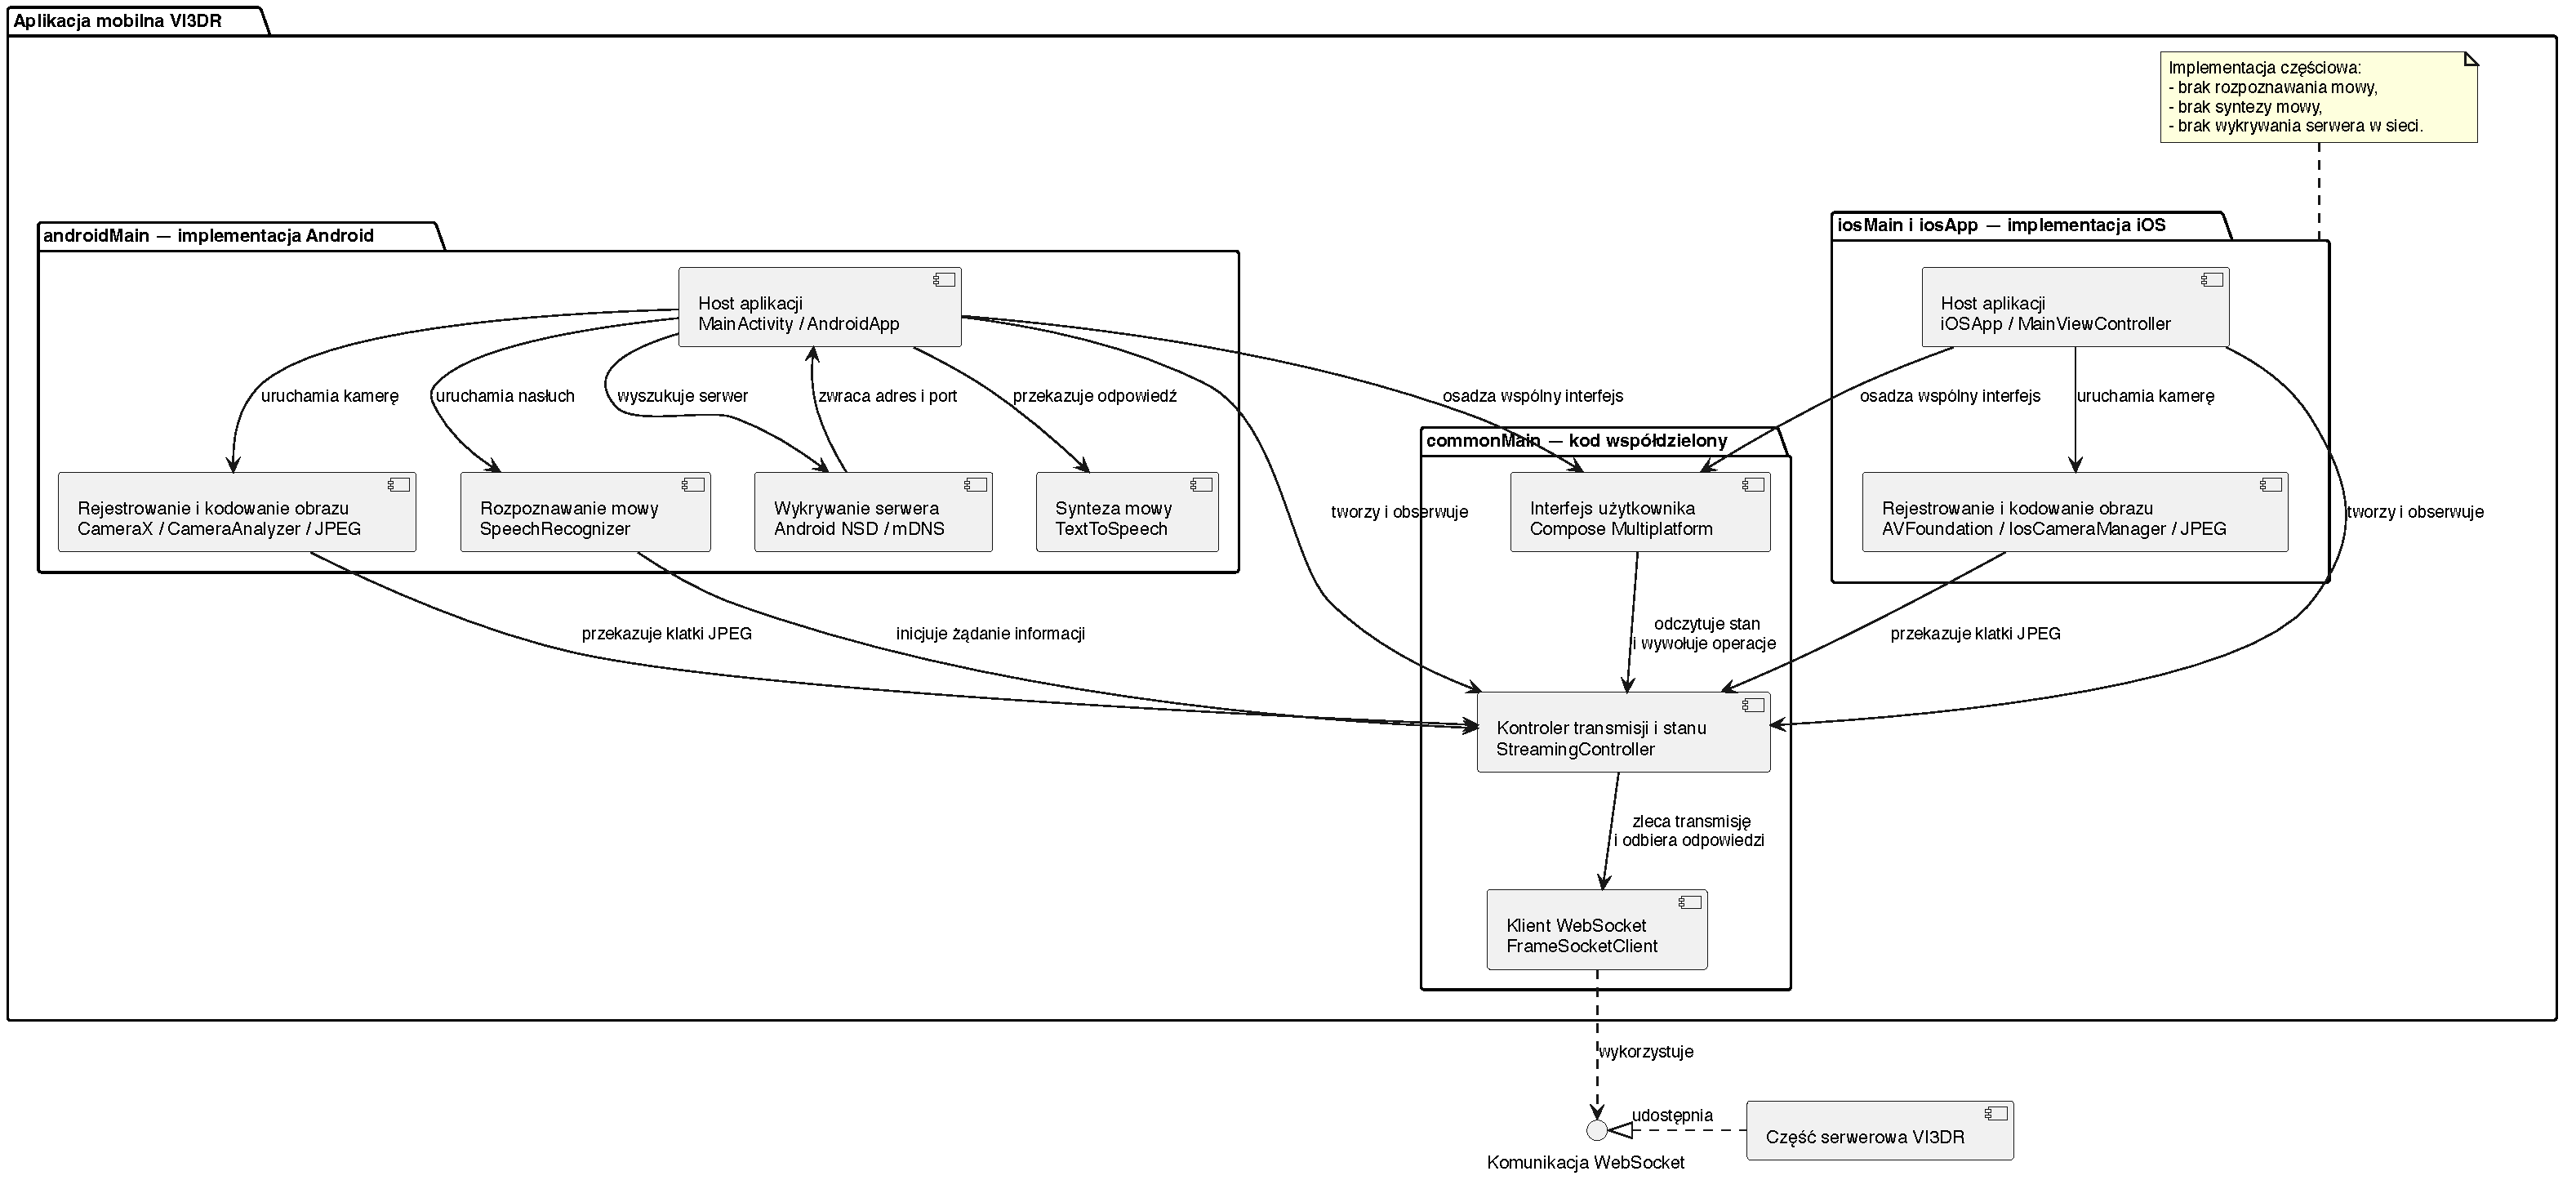
\includegraphics[
            width=\textheight,
            height=\linewidth,
            keepaspectratio]
            {./graf/diagram_mobilka.pdf}

        \captionof{figure}{Diagram komponentów aplikacji mobilnej z podziałem na kod współdzielony i implementacje platformowe}
        \label{fig:diagram_komponentow_aplikacji}
    \end{center}
    
\end{sidewaysfigure}

\clearpage

\subsection{Organizacja kodu aplikacji}

Implementacja aplikacji mobilnej została zrealizowana z wykorzystaniem technologii Kotlin Multiplatform i Compose Multiplatform. Kod aplikacji umieszczono w module \texttt{composeApp} i podzielono na pakiety odpowiadające częściom wspólnym i zależnym od platformy. W katalogu \texttt{commonMain} znajduje się kod współdzielony obsługujący logikę zarządzania stanem aplikacji, komunikację z serwerem, obsługę połączenia oraz wspólne elementy interfejsu użytkownika. Katalogi \texttt{androidMain} i \texttt{iosMain} zawierają implementacje korzystające z natywnych funkcji systemów Android i iOS, takich jak rejestrowanie obrazu, obsługa komend głosowych i odczytywanie komunikatów z serwera.

Centralny punkt aplikacji stanowi klasa \texttt{StreamingController}, zarządzająca stanem połączenia i transmisji. Kontroluje ona również częstotliwość przesyłania kolejnych klatek oraz obsługuje żądania użytkownika i odpowiedzi serwera. Stan kontrolera wykorzystywany jest przez interfejs użytkownika przygotowany w technologii Compose Multiplatform. Do współdzielonego interfejsu użytkownika dołączany jest natywny podgląd z kamery urządzenia.

Zastosowanie technologii Kotlin Multiplatform umożliwiło rozpoczęcie prac nad aplikacją mobilną jednocześnie dla systemów Android i iOS. Wstępne testy implementacji ukazały jednak istotne problemy ze stabilnością i wydajnością aplikacji na systemie iOS. Z tego względu dalsze prace skupiono wyłącznie na aplikacji dla systemu Android, dla której zaimplementowano wszystkie funkcjonalności systemu. Kod aplikacji dla systemu iOS pozostawiono w repozytorium aby umożliwić dalszy rozwój tej gałęzi w przyszłości.

\subsection{Rejestrowanie i przygotowanie obrazu}

Punktem wejścia do aplikacji jest klasa \texttt{MainActivity}, która uruchamia interfejs użytkownika i konfiguruje elementy wymagające dostępu do natywnych mechanizmów systemu: kamery, mikrofonu i syntezatora mowy. Rejestrowanie obrazu z kamery realizowane jest przy użyciu biblioteki CameraX, która udostępnia strumień kolejnych klatek. Ten obsługiwany jest mechanizmem \texttt{ImageAnalysis}, korzystając ze strategii \texttt{STRATEGY\_KEEP\_ONLY\_LATEST}. Przyjęcie jej sprawia, że w przypadku w którym aplikacja nie zdąży przetworzyć wszystkich klatek, zostaną one pominięte, a do przetwarzania zostanie wybrana najnowsza z nich. To podejście sprawia, że aplikacja nie generuje dodatkowego narzutu związanego z rosnącą długością kolejki obrazów i ogranicza opóźnienia pomiędzy pozycją bryły, a danymi przesyłanymi do serwera.

Klatki zarejestrowane z kamery są przetwarzane w klasie \texttt{CameraAnalyzer}. Dane przekazywane przez CameraX są konwertowane z formatu \texttt{YUV\_420\_888} do układu \texttt{NV21}, a następnie kompresowane do formatu JPEG. Wykorzystanie sieci bezprzewodowej do przesyłania danych premiuje kompresję danych, ponieważ obniża to wymagania dotyczące przepustowości łącza i zmniejsza opóźnienia w transmisji. Po zakończeniu przygotowania klatki jest ona przekazywana do dalszej obsługi, a obiekt \texttt{ImageProxy} jest zwalniany, by możliwe było przyjęcie kolejnych danych.

\subsection{Zarządzanie transmisją}
\label{ssec:zarzadzanie_transmisja}

Po przygotowaniu klatki, jest ona przekazywana do części wspólnej aplikacji. Każde wysłanie poprzedzone jest sprawdzeniem stanu połączenia: czy transmisja została aktywowana, czy połączenie z serwerem pozostaje otwarte, oraz czy wysłanie nie spowoduje przekroczenia ustalonego limitu FPS. Odbywa się to w klasie \texttt{StreamingController}, która przekazuje przygotowaną tablicę bajtów do wydzielonego klienta komunikacji. Rozdzielenie warstwy komunikacji od logiki aplikacji sprawia, że moduł kamery nie musi znać sposobu komunikacji z serwerem, a klient może być w przyszłości wymieniony na inny, np. w wypadku zmiany protokołu komunikacyjnego.

Interfejs użytkownika umożliwia włączanie i wyłączanie transmisji obrazu oraz zmianę parametrów połączenia. Są to: adres i port serwera, częstotliwość przesyłania klatek oraz jakość przesyłanego obrazu. Zrzut ekranu \ref{fig:interfejs_mobilka} przedstawia wygląd interfejsu aplikacji mobilnej. Komunikaty informujące o zmianie stanu połączenia są wyświetlane w formie toastów. Szczegóły protokołu komunikacyjnego, format wymienianych wiadomości oraz sposób nawiązywania połączenia są opisane w sekcji \ref{s:komunikacja} poświęconej komunikacji klient--serwer.

\begin{figure}[ht]
    \centering
    \includegraphics[width=0.85\textwidth]{example-image-duck}
    \caption{Interfejs aplikacji mobilnej}
    \label{fig:interfejs_mobilka}
\end{figure}

\subsection{Obsługa interakcji głosowej}
\label{ssec:interakcja_glosowa}

Interakcja z systemem została zrealizowana w sposób, który nie wymaga od użytkownika niewidomego korzystania z ekranu dotykowego. Wersja aplikacji dla systemu Android wykorzystuje wbudowane mechanizmy rozpoznawania mowy za pomocą mechanizmu \texttt{SpeechRecognizer} w klasie \texttt{VoiceCommandRecognizer}. Rozpoznany tekst analizowany jest pod kątem występowania komendy głosowej, a w przypadku jej wykrycia, kontroler aplikacji wysyła do serwera odpowiednie żądanie. Obecna wersja aplikacji obsługuje jedynie komendy żądania informacji i nie przewiduje możliwości sterowania transmisją obrazu. Przyszłe wersje systemu mogą zostać rozbudowane o te funkcjonalności, ale założenie projektowe przewiduje, że osoba niewidoma będzie korzystała z systemu w towarzystwie osoby widzącej, mogącej sterować transmisją obrazu.

Odpowiedzi otrzymywane z serwera są zapisywane w stanie aplikacji, a następnie przekazywane do mechanizmu \texttt{TextToSpeech}. Syntezator mowy odczytuje komunikaty z serwera w języku urządzenia. Jego wykorzystanie uniezależnia użytkownika od konieczności wejścia w interakcję z ekranem dotykowym podczas żądania i odbierania informacji.

Mechanizmy rozpoznawania i syntezy mowy są silnie zależne od platformy i systemu operacyjnego. Inicjacja żądania i obsługa treści odpowiedzi odbywa się jednak w części wspólnej aplikacji. Umożliwia to w przyszłości rozszerzenie aplikacji o kolejne systemy, bez konieczności ponownej implementacji sposobu komunikacji z serwerem.

\section{Implementacja części serwerowej}
\label{s:implementacja_serwera}

Część serwerowa odpowiada za odbieranie danych z aplikacji mobilnej, dekodowanie ich, wykonywanie detekcji obiektów i prezentowanie stanu systemu. Do jej przygotowania wykorzystano język Python i można ją uruchomić w formie aplikacji konsolowej lub z interfejsem graficznym.

\subsection{Organizacja i uruchamianie serwera}

Głównym punktem wejścia do serwera jest klasa \texttt{ApplicationRuntime}, której zadaniem jest utworzenie i połączenie modułów: serwera WebSocket, modułu detekcji obiektów oraz komponentu publikującego usługę w sieci lokalnej. W procesie uruchamiania serwera wczytywany jest model detekcji, funkcja wykonująca inferencję przekazywana jest do modułu obsługi obrazów i uruchamiane są mechanizmy komunikacji i publikacji usługi. W przypadku uruchomienia serwera z interfejsem graficznym, główny wątek aplikacji obsługuje interfejs Qt, a osobny wątek z własną pętlą zdarzeń \texttt{asyncio} obsługuje właściwy serwer. Dzięki temu, że oba sposoby uruchamiania serwera korzystają z tej samej klasy \texttt{ApplicationRuntime}, sposób działania nie jest zależny od wyboru interfejsu.

Kod odpowiedzialny za połączenia został rozdzielony na dwa poziomy. Serwer WebSocket jest zarządzany przez klasę \texttt{CaptureServer}, która odpowiada również za kontrolę aktywnej sesji. Dla każdego klienta jest natomiast tworzona instancja klasy \texttt{CaptureSession}, odpowiadajaca za obsługę wiadomości i przetwarzanie przychodzących obrazów.

Ustawienia serwera zgromadzono w pliku \texttt{settings.py}, gdzie możliwe jest wprowadzenie zmian dotyczących adresu i portu serwera, parametrów kolejki, konfiguracji mDNS oraz modelu detekcji. Ustawienia dotyczące bezpośrednio detekcji, jak jej próg pewności, rozmiar obrazu wejściowego i urządzenie wykorzystywane do obliczeń są przekazywane do modułu detekcji w momencie jego tworzenia. Zmiana tych parametrów wymaga ponownego uruchomienia serwera.

Możliwa jest wymiana modelu detekcji na inny bez konieczności modyfikacji pozostałych elementów systemu. Wariant z interfejsem użytkownika umożliwia wybranie modelu z pliku \texttt{.pt}, korzystając z systemowego okna dialogowego. Jest on następnie ładowany przez klasę \texttt{YOLODetector}. Obiekt detektora nie jest zmieniany, więc sesje odwołują się do tej samej funkcji przetwarzającej, ale kolejne iteracje detekcji wykonywane są na nowym modelu. Wariant konsolowy wymaga podania ścieżki do modelu w pliku konfiguracyjnym i ponownego uruchomienia serwera.

Podczas tworzenia obiektu \texttt{ApplicationRuntime} wczytywana jest również przygotowana wcześniej baza wiedzy zawierająca informacje o powierzchniach brył oraz odpowiadające im informacje. Dane przechowywane są w pojedynczym pliku \texttt{.json} o ustalonej strukturze. Loader przekształca zawartość pliku do struktur danych reprezentujących bryły, powierzchnie i parametry dopasowania kolorów. Baza może zostać przeładowana w trakcie działania serwera, a przy obsłudze kolejnych żądań informacji wykorzystywana jest nowa konfiguracja.

\subsection{Odbieranie i przygotowanie obrazu}
\label{ssec:odb_prz_obrazu}

Po nawiązaniu połączenia z klientem klasa \texttt{CaptureServer} tworzy obiekt \texttt{CaptureSession} do którego przekazuje funkcję wykonującą detekcję. Uruchomiona zostaje asynchroniczna pętla odbioru wiadomości. Jeżeli serwer rozpozna wiadomość binarną, jest ona traktowana jako klatka obrazu i przekazywana do dalszej obsługi.

Aby ograniczyć liczbę zaległych klatek, rozmiar kolejki wejściowej ustawiono na pojedynczą wiadomość. Metoda \texttt{\_drain\_to\_latest\_frame} sprawdza, czy w kolejce znajdują się kolejne dane binarne, a jeżeli tak, to zastępuje starszy obraz nowszym. Taki mechanizm nie gwarantuje zachowania wszystkich klatek, ale zmniejsza ryzyko wykonania detekcji na obrazie, który nie jest już aktualny i nie odpowiada aktualnemu położeniu bryły. Jeżeli serwer nie zdąży przetworzyć starszych klatek są one pomijane, a do detekcji przekazywana jest najnowsza z nich.

Wiadomości binarne są wstępnie sprawdzane pod kątem występowania plików JPEG na podstawie dwóch pierwszych bajtów \texttt{FF D8}. Następnie są one przekazywane do tablicy \texttt{NumPy}, gdzie dekodowane są do formatu z kanałami BGR korzystając z funkcji \texttt{cv2.imdecode}. W przypadku niepowodzenia dana wiadomość zostaje pominięta bez przerywania sesji. Poprawnie zdekodowany obraz jest przekazywany do modelu detekcji. Po zakończeniu predykcji wynik zostaje zapisany razem z kopią odpowiadającej mu klatki obrazu w strukturze \texttt{DetectionSnapshot}. Dzięki temu przechowywana jest spójna para obrazu i wyniku wykonanej na nim detekcji. Dostęp do aktualnego snapshotu chroniony jest blokadą wątkową, aby nie było możliwe jednoczesne zapisywanie i odczytywanie danych. 

W chwili otrzymania żądania informacji pobierany jest najnowszy kompletny \texttt{DetectionSnapshot}. Dalsza analiza oparta jest na informacjach w nim zawartych, a kolejne obrazy mogą być niezależnie odbierane i przetwarzane przez serwer.

Wynikiem przetwarzania, zwracanym przez model, jest między innymi klatka z naniesionymi ramkami detekcji, która wykorzystywana jest w oknie podglądu. Częstotliwość z jaką aktualizowany jest podgląd nie jest zależna od inferencji. Brak aktualizacji podglądu nie oznacza, że nie została wykonana detekcja, a jedynie, że nie zdążyła ona zostać wyświetlona w interfejsie.

\subsection{Moduł detekcji obiektów}

Ładowaniem i wykonywaniem detekcji obiektów zajmuje się klasa \texttt{YOLODetector}. W momencie jej inicjalizacji otrzymuje ona ścieżkę do modelu, minimalną wartość pewności detekcji, rozmiar obrazu wejściowego oraz urządzenie wykorzystywane do obliczeń. Model jest ładowany przy użyciu klasy \texttt{YOLO} z biblioteki \texttt{Ultralytics}. Wśród dostępnych urządzeń do obliczeń można wybrać warianty udostępniane przez bibliotekę \texttt{PyTorch}, w tym CPU, GPU i \texttt{MPS}. Domyślnie, w przypadku braku wyboru urządzenia, ten zostaje wybrany automatycznie przez biblioteki. Inferencja modelu odbywa się poprzez uruchomienie metody \texttt{annotate} w której obraz przekazywany jest do funkcji \texttt{model.predict} razem z parametrami wynikającymi z konfiguracji.

Istnieje możliwość, że w wyniku detekcji na obrazie zostanie oznaczonych wiele obiektów. W takim przypadku wykorzystywana jest metoda \texttt{\_extract\_best\_detection}, która wybiera detekcję o najwyższej wartości pewności. Następnie pobiera z niej informacje o klasie obiektu oraz jego współrzędnych na obrazie w postaci

\begin{equation}
    B = (x_1,y_1,x_2,y_2)
\end{equation}
ograniczonych do wymiarów obrazu. Eliminuje to możliwość wyznaczenia obszaru znajdującego się poza jego granicami.

Informacje o obiekcie są przechowywane w strukturze \texttt{DetectionResult}, która zawiera nazwę przewidywanej klasy, wartość pewności detekcji i obiekt \texttt{DetectionBox} z informacjami o położeniu ramki ograniczającej. Struktura ta posiada metodę, która umożliwia wyodrębnienie z obrazu fragmentu odpowiadającego zapisanej ramce. Po zakończeniu predykcji tworzony jest obiekt \texttt{DetectionSnapshot}, zawierający kopię przetworzonej klatki oraz odpowiadający jej \texttt{DetectionResult}. Oba elementy wykorzystują blokadę wątkową zapisu i odczytu, aby zapobiec sytuacji, w której podczas przygotowywania odpowiedzi wykorzystana zostałaby klatka pochodząca z innej iteracji modelu detekcji. Snapshot zostaje zaktualizowany po każdej zakończonej predykcji i może zostać pobrany w chwili żądania informacji.

Ładowanie modelu i wykonywanie detekcji również są operacjami chronionymi blokadą wątkową, aby uniknąć sytuacji, w której model mógłby zostać nadpisany w trakcie wykonywania predykcji.

\subsection{Analiza wycinka i przygotowanie informacji zwrotnej}

Szczegółowa analiza obiektu jest wykonywana wyłącznie po otrzymaniu żądania informacji od klienta. Dzięki temu detekcja pozostaje oddzielona od pozostałych operacji wymaganych jedynie do przygotowania informacji zwrotnej. Odebranie komunikatu \texttt{info-request} skutkuje utworzeniem obiektu \texttt{AnalysisContext}, przechowującego najnowszy kompletny \texttt{DetectionSnapshot} oraz referencję do bazy wiedzy. Dzięki takiemu mechanizmowi późniejsze procesy nie wpływają na już rozpoczętą analizę.

Analiza wykonywana jest używając klasy \texttt{AnalysisWorker}. Wykorzystuje ona osobny wątek w obiekcie \texttt{ThreadPoolExecutor}, dzięki czemu może wykonywać obliczenia poza główną pętlą zdarzeń serwera. W ramach zadania, na podstawie wyniku detekcji w kontekście, wyodrębniany jest fragment obrazu ograniczony ramką detekcji. Jeżeli snapshot nie istnieje, model nie wykrył obiektu lub wycinek jest niepoprawny, dalsza analiza nie jest wykonywana.

Właściwe przetwarzanie wycinka obrazu odbywa się w klasie \texttt{SliceAnalyzer}. Jako parametry otrzymuje ona wycinek obrazu, nazwę rozpoznanej klasy obiektu oraz bazę wiedzy. Klasa służy jedynie do pobrania odpowiednich informacji o powierzchniach bryły i dopasowaniu kolorów. Niweluje to sposobność powielania obliczeń dla obiektów, których nie dotyczy analiza. 

Rozpoznanie widocznej powierzchni odbywa się w module \texttt{SurfaceMatcher}. Do każdej powierzchni w bazie wiedzy dopasowywany jest kolor referencyjny zapisany jako nazwa koloru CSS oraz komunikat informacyjny. Nazwa koloru jest przekształcana do przestrzeni RGB, a następnie do układu BGR i przestrzeni Lab. Wycinek obrazu również jest przekształcany do przestrzeni Lab, a następnie wykonywane jest dopasowanie kolorów. Odbywa się ono dla każdego piksela wycinka poprzez obliczenie kwadratu odległości euklidesowej od kolorów referencyjnych wszystkich powierzchni. Piksel jest przypisywany do koloru wyłącznie wtedy, gdy uzyskana odległość jest mniejsza od ustalonego progu \texttt{max\_distance} znajdującego się w konfiguracji bryły. Następnie zliczana jest liczba pikseli należących do każdej z powierzchni. Wynikiem jest informacja o powierzchni, której kolor został dopasowany do największej liczby pikseli wycinka. 

Po określeniu powierzchni \texttt{SliceAnalyzer} zwraca komunikat informacyjny, który następnie jest przekazywany do klienta. Jeżeli zajdzie błąd w trakcie analizy, np. nie zostanie wykryta powierzchnia, klient otrzymuje komunikat: "Nie udało się rozpoznać widocznej powierzchni". 

\subsection{Organizacja przetwarzania współbieżnego}

Obsługa serwera i sesji odbywa się w pętli zdarzeń biblioteki \texttt{asyncio}. Operacje sieciowe realizowane są w sposób asynchroniczny, dzięki czemu oczekiwanie na nie nie blokuje procesu serwera.

Operacje, których wykonanie może trwać dłużej od pozostałych, a tym samym mogące blokować pętlę zdarzeń są wykonywane poza głównym wątkiem serwera. Wykorzystują one mechanizm \texttt{asyncio.to\_thread}, a należą do nich: ładowanie modelu, inferencja, rejestrowanie i wyrejestrowanie usługi w sieci lokalnej. Inferencja, mimo oddzielnego wątku, pozostaje operacją sekwencyjnego przepływu obrazu -- sesja oczekuje na jej zakończenie zanim rozpocznie kolejną iterację.

Odmienne podejście przyjęto w przypadku analizy wycinka obrazu uruchamianej na żądanie klienta. Tutaj, po otrzymaniu żądania, synchronicznie tworzony jest obiekt kontekstu analizy. Następnie tworzone jest nowe zadanie \texttt{asyncio}, a obliczenia są przekazywane do klasy workera. Wykorzystuje on obiekt \texttt{ThreadPoolExecutor} z pojedynczym wątkiem, co nie blokuje głównej pętli zdarzeń serwera. W czasie wykonywania analizy, serwer może odbierać kolejne klatki i wykonywać na nich detekcję obiektów. Nie wpływa to na rozpoczętą analizę, ponieważ korzysta ona ze snapshotu zapisanego w kontekście w momencie otrzymania żądania. Po zakończeniu pracy wynik powraca do pętli zdarzeń, gdzie następuje jego dalsza obsługa. Zamknięcie sesji skutkuje anulowaniem wszystkich zadań analizy, które nie zostały jeszcze zakończone.

Wariant desktopowy dzieli przetwarzanie na dwa wątki wykonania. Główny wątek obsługuje interfejs graficzny, a backend uruchamiany jest w osobnym wątku z własną pętlą zdarzeń. Operacje wykonywane na interfejsie graficznym przez użytkownika są przekazywane do backendu poprzez mechanizm korutyn biblioteki \texttt{asyncio}. Dane przekazywane z backendu do interfejsu graficznego są emitowane w formie sygnałów Qt. Stan współdzielony jest chroniony blokadą wątkową.

\subsection{Interfejs graficzny}

Do przygotowania interfejsu graficznego wykorzystano bibliotekę \texttt{PySide6}, Qt WebEngine i mechanizm \texttt{QWebChannel}. Warstwa prezentacji przygotowana jest w technologiach webowych: HTML, CSS i JavaScript. Komunikacja między interfejsem a backendem jest realizowana przez obiekt \texttt{DesktopBridge}.

Klasą utrzymującą informacje dotyczące działania serwera jest \texttt{BackendController}, która pośredniczy w wymianie danych między interfejsem Qt a backendem. Do jej zadań należy odbiór obrazu podglądu, klasy obiektu, wartości pewności detekcji, stanu sesji i metryk transmisji. Dane, które mają zostać zaprezentowane użytkownikowi są następnie przekazywane do warstwy JavaScript z wykorzystaniem sygnałów Qt.

Obraz podglądu jest kodowany do JPEG i przekazywany do interfejsu w formie adresu danych w formacie Base64. Takie podejście niweluje konieczność zapisu danych na dysku. Informacje o wynikach detekcji są przekazywane oddzielnie, a częstotliwość ich aktualizacji została ograniczona w celu zmniejszenia narzutu związanego z renderowaniem interfejsu.

Aplikacja umożliwia obserwowanie stanu backendu, aktywnej sesji, parametrów obrazu i metryk transmisji. Udostępnia również możliwość zmiany modelu detekcji, a także wysłania wiadomości do klienta wykorzystując metodę służącą do przesyłania informacji. Zrzut ekranu \ref{fig:interfejs_serwera} przedstawia wygląd interfejsu graficznego serwera.

\begin{figure}[ht]
    \centering
    \includegraphics[width=0.85\textwidth]{example-image-duck}
    \caption{Interfejs graficzny serwera}
    \label{fig:interfejs_serwera}
\end{figure}

\subsection{Obsługa błędów i cykl życia}
\label{ssec:bledy}

Podczas uruchomienia serwera, przed udostępnieniem możliwości nawiązania połączenia, ładowany jest model detekcji i rejestrowana jest usługa sieciowa mDNS. Niepowodzenie wykonania jednego z tych procesów skutkuje wyświetleniem komunikatu o błędzie i zakończeniem uruchamiania backendu. W wariancie desktopowym, komunikat o błędzie jest wyświetlany na interfejsie użytkownika.

Problemy dotyczące pojedynczej klatki nie są przyczyną przerwania sesji. W przypadku zaistnienia nieobsługiwanych danych przesyłanych przez klienta, serwer ignoruje je i kontynuuje działanie. Przy błędzie modułu detekcji do interfejsu przekazywana jest klatka bez naniesionych ramek detekcji, komunikat o błędzie pojawia się w logach serwera, a serwer kontynuuje pracę i obsługę kolejnych klatek.

Obsługa żądania informacji przewiduje typowe sytuacje uniemożliwiające wykonanie analizy wycinka. Wystąpienie błędu nie zatrzymuje działania serwera, a skutkuje jedynie przygotowaniem komunikatu zastępczego. Wyjątki związane bezpośrednio z odczytem bazy wiedzy i dopasowaniem powierzchni są obsługiwane w module analizy. Nieprzewidziane wyjątki w trakcie zadania analizy są odnotowane w logach serwera, ale w tym wypadku do klienta nie jest wysyłany żaden komunikat o wystąpieniu błędu. 

Rozłączeniu klienta towarzyszy zamknięcie podglądu w interfejsie serwera, wyzerowanie metryk sesji i usunięcie ostatniego obrazu z interfejsu. Anulowane zostają aktywne zadania analizy, a przypisany worker zostaje zatrzymany. Informacje o aktywnej sesji są zwalniane i możliwe jest nawiązanie połączenia z kolejnym klientem. Zatrzymanie serwera skutkuje zamknięciem mechanizmu WebSocket i wyrejestrowaniem usługi w sieci lokalnej. Następnie następuje zakończenie wszystkich wątków i zamknięcie procesu aplikacji. Wariant desktopowy w pierwszej kolejności kończy działanie wątku backendu, a następnie zamyka interfejs graficzny Qt.

\section{Komunikacja klient--serwer}
\label{s:komunikacja}

Komunikacja z serwerem, zgodnie z założeniami projektowymi, odbywa się w architekturze klient--serwer. Do jej realizacji wykorzystano protokół WebSocket, umożliwiający stałą komunikację dwukierunkową. Dzięki wykorzystaniu tego protokołu, możliwe jest przesyłanie kolejnych klatek oraz komunikatów sterujących pojedynczym kanałem komunikacyjnym, bez konieczności ponownego nawiązywania połączenia dla każdej wiadomości.

Do implementacji komunikacji aplikacja mobilna wykorzystuje bibliotekę \texttt{Ktor}, a część serwerowa bibliotekę \texttt{websockets}. Szczegóły implementacyjne przygotowania i przetwarzania obrazu przedstawiono w sekcjach \ref{s:implementacja_aplikacji} i \ref{s:implementacja_serwera}. Niniejsza sekcja skupia się na opisie wymiany danych pomiędzy rozproszonymi modułami systemu.

\subsection{Nawiązywanie połączenia i wykrywanie serwera}

Aby możliwe było połączenie z serwerem konieczna jest znajomość jego adresu IP i portu. Można je wprowadzić ręcznie korzystając z pól interfejsu użytkownika, lub skorzystać z mechanizmu wykrywania usług w sieci lokalnej.

Aplikacja przeznaczona na system Android wykorzystuje mechanizm Network Service Discovery (NSD), oparty na protokole mDNS. Serwer publikuje usługę typu \texttt{\_vi3dr.\_tcp.local.} w sieci lokalnej pod nazwą \texttt{VI3DR Server}. Po uruchomieniu wyszukiwania w aplikacji mobilnej i odnalezieniu usługi, pobrane zostają przypisane do niej adres IP i numer portu, które następnie przekazane do kontrolera transmisji automatycznie uzupełniają konfigurację połaczenia.

Publikacji usługi po stronie serwera realizowana jest za pomocą biblioteki \texttt{zeroconf}. W rekordzie zawarte są również dodatkowe informacje dotyczące protokołu, wersji i ścieżki połączenia, aczkolwiek aktualna implementacja nie wykorzystuje ich w żaden sposób. W przyszłości mogą one zostać użyte do weryfikacji zgodności wersji i umożliwienia współpracy różnych wersji poszczególnych komponentów systemu.

Na podstawie odczytanych parametrów tworzony jest adres serwera w postaci \texttt{ws://<adres\_ip>:<port>}. Po rozpoczęciu transmisji aplikacja nawiązuje połączenie z serwerem i tworzy sesję obsługiwaną w klasie \texttt{FrameSocketClient}. Poprawne ustanowienie sesji skutkuje zmianą stanu na \textit{połączony} i od tego momentu możliwe jest wysyłanie kolejnych klatek obrazu oraz równoległa wymiana komunikatów sterujących w postaci wiadomości tekstowych.

Serwer domyślnie nasłuchuje na porcie 8765, na wszystkich dostępnych interfejsach sieciowych, obsługując jednocześnie pojedynczą sesję. W przypadku próby nawiązania połączenia przez kolejnego klienta, serwer odrzuca je wysyłając komunikat \texttt{client\_stop} i zamykając połączenie (por. \ref{s:ograniczenia}).

\subsection{Protokół i format przesyłanych danych}

W ramach połączenia, pomiędzy klientem a serwerem, wymieniane są wiadomości w formacie binarnym i tekstowym. Podstawowe wiadomości protokołu zostały przedstawione w tabeli \ref{tab:komunikaty_protokolu}.

\begin{table}[htbp]
    \centering
    \caption{Podstawowe komunikaty protokołu klient--serwer}
    \label{tab:komunikaty_protokolu}
    \begin{tabularx}{\textwidth}{lllX}

        \toprule

        \textbf{Kierunek}           &
        \textbf{Typ}                &
        \textbf{Format}             &
        \textbf{Znaczenie}                                                                                                                        \\

        \midrule

        Klient $\rightarrow$ serwer &
        binarny                     &
        dane JPEG                   &
        Klatka obrazu zarejestrowana przez kamerę urządzenia mobilnego.                                                                           \\

        \addlinespace

        Klient $\rightarrow$ serwer &
        tekstowy                    &
        \texttt{info-request}       &
        Żądanie przygotowania informacji dotyczącej aktualnie eksplorowanego obiektu.                                                             \\

        \addlinespace

        Klient $\rightarrow$ serwer &
        tekstowy                    &
        \texttt{stop}               &
        Żądanie zakończenia transmisji i zamknięcia aktywnej sesji.                                                                               \\

        \addlinespace

        Serwer $\rightarrow$ klient &
        tekstowy                    &
        \makecell[tl]{\texttt{info-response:}                                                                                                     \\\texttt{<tekst>}} &
        Tekst przeznaczony do odczytania użytkownikowi, zawierający informację o obiekcie albo komunikat o problemie z przygotowaniem odpowiedzi. \\

        \addlinespace


        Serwer $\rightarrow$ klient &
        tekstowy                    &
        \texttt{client\_stop}       &
        Polecenie zakończenia połączenia wysyłane przez część serwerową.                                                                          \\

        \bottomrule
    \end{tabularx}
\end{table}

Wiadomość binarna zawiera wyłącznie bajty obrazu zakodowanego w formacie JPEG. Zrezygnowano z dodatkowego nagłówka warstwy aplikacji i metadanych, mogących zawierać informacje o rozdzielczości obrazu, numerze klatki czy znaczniku czasu, ponieważ nie są one wymagane do prawidłowego działania systemu. Typ wiadomości protokołu WebSocket pozwala na odróżnienie danych obrazu od komunikatów sterujących, jednakże po stronie serwera sprawdzane są dwa początkowe bajty obrazu -- charakterystyczne dla formatu JPEG. Zawartość wiadomości jest następnie przekazywana do dalszego przetwarzania.

Komunikaty sterujące mają postać tekstową i są przesyłane w formacie UTF-8. Rozwiązanie to ogranicza złożoność protokołu i pozwala na łatwe rozróżnienie poszczególnych operacji.

\subsection{Przesyłanie klatek obrazu}

Po przygotowaniu obrazu przez aplikację mobilną, jest on przechowywany w formie tablicy bajtów JPEG. Przed wysłaniem kontroler sprawdza, czy transmisja jest aktywna, czy połączenie z serwerem pozostaje otwarte, oraz czy wysłanie nie spowoduje przekroczenia ustalonego limitu FPS. Jeżeli wszystkie warunki są spełnione, obraz jest przekazywany do serwera w formie wiadomości binarnej (por. \ref{ssec:zarzadzanie_transmisja}).

Serwer, po odebraniu wiadomości binarnej, przekazuje ją do obiektu \texttt{CaptureSession}. W przypadku nagromadzenia wielu klatek preferowana jest najnowsza z nich. Szczegóły implementacyjne tego mechanizmu zostały opisane w sekcji \ref{ssec:odb_prz_obrazu}.

Warstwa aplikacji nie implementuje ponownego przetwarzania pominiętych klatek -- nie jest to wymagane, ponieważ nowsze klatki zastępują starsze. Protokół WebSocket korzysta z transportu TCP, zapewniającego uporządkowanie dostarczenia przesyłanych wiadomości.

\subsection{Obsługa komunikatów sterujących}

Poza wiadomosciami binarnymi w systemie wymieniane są również komunikaty sterujące w formie tekstowej. Odpowiadają one za obsługę żądań użytkownika oraz cyklu życia transmisji.

Po rozpoznaniu komendy głosowej aplikacja przekazuje do serwera wiadomość \texttt{info-request}. Jej odebranie przez serwer skutkuje zakolejkowaniem zadania przygotowania tekstu zawierającego informacje zwrotne. Obsługa kończy się bez oczekiwania na rezultat, aby nie blokować potoku i by sesja mogła kontynuować swoje działanie.

Końcowym etapem analizy obiektu jest przekazanie przygotowanego przez moduł tekstu z powrotem do sesji, a następnie jego wysłanie w postaci \texttt{info-response:<tekst>}. Aplikacja kliencka rozpoznaje prefiks odpowiedzi i przekazuje zawartość do dalszej obsługi w kontrolerze. Ostatecznie tekst zostaje przekazany do mechanizmu syntezatora mowy opisanego w sekcji \ref{ssec:interakcja_glosowa}.

\subsection{Cykl życia połączenia i obsługa błędów}

Po ustanowieniu sesji możliwe jest rozpoczęcie komunikacji aplikacji z serwerem, poprzez przekaz kolejnych klatek obrazu i wymianę komunikatów sterujących. Jeżeli użytkownik pragnie zakończyć transmisję, aplikacja wysyła do serwera wiadomość \texttt{stop} inicjując zamknięcie sesji. Połączenie może również zostać zakończone przez serwer poprzez wysłanie do aplikacji komunikatu \texttt{client\_stop}. Stosuje się go w przypadku próby połączenia kolejnego klienta lub zamknięcia procesu serwera. W obu przypadkach aplikacja mobilna zmienia stan na \textit{rozłączony} i wyświetla komunikat o zakończeniu sesji.

Błąd podczas łączenia z serwerem powoduje przejście aplikacji do stanu błędu i wyświetlenie komunikatu. Nie są wykonywane automatyczne próby ponownego połączenia, więc wznowienie transmisji wymaga ręcznej interwencji użytkownika.

Błędy pojedynczych wiadomości są izolowane i nie powodują przerwania sesji. Niepoprawne dane binarne są pomijane, a szczegółowe informacje dotyczące zachowania serwera w przypadku błędów zostały opisane w sekcji \ref{ssec:bledy}.

Komunikacja odbywa się przy użyciu nieszyfrowanego wariantu protokołu WebSocket i nie wykorzystuje mechanizmu uwierzytelniania klienta. Takie podejście zostało uznane za wystarczające w kontekście pracy w zaufanej sieci lokalnej. W przyszłości możliwe jest rozszerzenie protokołu o mechanizmy szyfrowania i uwierzytelniania, gdyby system miał zostać wykorzystany w sieciach publicznych.

\section{Narzędzia pomocnicze}

Oprócz aplikacji mobilnej i serwera, aby możliwe było przygotowanie zbioru danych, uczenie modeli i przeprowadzenie eksperymentów, przygotowano zestaw narzędzi pomocniczych. Nie uczestniczą one bezpośrednio w działaniu systemu, ale umożliwiają przygotowanie jego najważniejszego elementu -- modelu detekcji obiektów. Zostały one przygotowane w języku Python i podzielone pomiędzy katalogi \texttt{video\_to\_dataset}, \texttt{dataset\_splitter} oraz \texttt{training}. Większość z nich udostępnia interfejs wiersza poleceń z możliwością podania parametrów działania bez konieczności modyfikacji kodu źródłowego.

\subsection{Ekstrakcja klatek z nagrań}
\label{ssec:extractor}

Do ekstrakcji klatek z nagrań wideo przygotowano skrypt znajdujący się w katalogu \texttt{video\_to\_dataset}. Jego zadaniem jest załadowanie pliku wideo i zapisanie kolejnych klatek w postaci osobnych plików graficznych. Do realizacji wykorzystano bibliotekę \texttt{OpenCV}.

Nagranie otwierane jest przez klasę \texttt{VideoCapture}, a następnie odczytywane są jego kolejne klatki. Użytkownik może określić częstotliwość zapisu klatek za pomocą parametru wejściowego. Dla wartości $n$ zapisywana jest pierwsza klatka, a następnie co $n$-ta klatka. Jeżeli nie zostanie podana wartość parametru, zachowana zostaje każda klatka filmu.

Obrazy zapisywane są zgodnie ze schematem \texttt{frame\_<n>.jpeg} w formacie JPEG. Jeżeli w katalogu docelowym znajdują się już jakieś pliki, narzędzie sprawdza ich nazwy i kontynuuje numerację od najwyższego numeru. Umożliwia to wielokrotne uruchamianie ekstrakcji z różnych nagrań w tym samym katalogu, bez ryzyka nadpisania istniejących plików.

Narzędzie nie modyfikuje w żaden sposób ekstrahowanych klatek, a zwraca obrazy bezpośrednio odczytane przez bibliotekę. Nie generuje również żadnych adnotacji, ponieważ ich przygotowanie odbywa się w osobnym procesie.

\subsection{Narzędzie do podziału zbioru danych}
\label{ssec:dataset_splitter}

Do organizacji zbioru danych przygotowano narzędzie \texttt{dataset\_splitter}. Jego zadaniem jest podział zbioru danych na dwie części: treningową i walidacyjną. Jako dane wejściowe przyjmowany jest katalog z obrazami i odpowiadającymi im adnotacjami w formacie YOLO. Dla każdego obrazu narzędzie wyszukuje odpowiadający mu plik z adnotacją, a jeżeli nie zostanie on odnaleziony obraz traktowany jest jako tło i tworzony jest dla niego pusty plik adnotacji.

Podział realizowany jest za pomocą funkcji \texttt{train\_test\_split} z biblioteki \texttt{scikit-learn}. Dane są losowane z zachowaniem stratyfikacji względem klasy, a wartość ziarna generatora liczb pseudolosowych może zostać określona przez użytkownika. Wynik działania narzędzia to drzewo katalogów odpowiadające strukturze w formacie YOLO:

\begin{itemize}
    \item \texttt{images/train},
    \item \texttt{images/val},
    \item \texttt{labels/train},
    \item \texttt{labels/val}.
\end{itemize}

Domyślny sposób działania narzędzia przewiduje kopiowanie plików do katalogów docelowych, ale możliwe jest również jego uruchomienie w trybie przenoszenia plików.

\subsection{Narzędzia do treningu i testowania modeli}

Najbardziej rozbudowanym narzędziem pomocniczym jest zestaw skryptów do treningu i testowania modeli detekcji, znajdujący się w katalogu \texttt{training}. Jego głównym punktem wejścia jest skrypt \texttt{train.py}, który uruchamia proces uczenia modelu wykorzystując bibliotekę \texttt{Ultralytics}.

Skrypt umożliwia wskazanie pliku konfiguracji zbioru danych oraz modelu używanego jako punkt początkowy. Możliwe jest użycie istniejących wag modelu, zapisanych w pliku \texttt{.pt}, lub rozpoczęcie treningu od zera, na podstawie architektury opisanej w pliku \texttt{.yaml}. Istnieje również możliwość kontynuowania treningu na podstawie wcześniej zapisanego punktu kontrolnego. Parametry uczenia mogą zostać zmienione przy uruchomieniu skryptu korzystając z argumentów wiersza poleceń. Zmianie podlegają między innymi: rozmiar obrazu wejściowego, rozmiar batcha, liczba epok, liczba procesów roboczych, wartość patience, urządzenie obliczeniowe oraz ścieżka katalogu wynikowego. Brak podania parametrów skutkuje uruchomieniem treningu z wartościami domyślnymi. Urządzenie wykorzystywane do obliczeń jest wybierane na podstawie dostępności technologii: CUDA, MPS, a następnie CPU.

Przed rozpoczęciem treningu sprawdzana jest poprawność konfiguracji zbioru danych w której wymagane są informacje o klasach oraz ścieżkach do katalogów z obrazami i adnotacjami dla zbiorów treningowego i walidacyjnego. Na potrzeby biblioteki tworzona jest następnie znormalizowana wersja konfiguracji, zapisywana w katalogu wynikowym.

Nieprawidłowości przy konfiguracji skutkują przerwaniem skryptu uniemożliwiając rozpoczęcie treningu. Możliwe jest sprawdzenie poprawności konfiguracji bez uruchamiania procesu uczenia korzystając z flagi \texttt{--dry-run}.

Uczenie modelu wykonywane jest przez metodę \texttt{model.train} z biblioteki \texttt{Ultralytics}. Odpowiada ona za kolejne epoki treningowe, walidację, tworzenie punktów kontrolnych i zapisywanie wyników. Główne pliki tworzone podczas uczenia to \texttt{results.csv}, wagi \texttt{best.pt} i \texttt{last.pt} oraz wykresy przebiegu uczenia.

Ocena modelu na wydzielonym zbiorze testowym jest realizowana przez skrypt \texttt{test.py}. Wykorzystuje on metodę walidacji z biblioteki \texttt{Ultralytics} z ustawieniem \texttt{split=test}. Wynikiem działania skryptu jest katalog \texttt{test} zawierający artefakty generowane przez bibliotekę, wśród których znajdują się między innymi macierze pomyłek i krzywe zależności.

Narzędzie udostępnia również skrypt \texttt{predict.py}, który umożliwia wykonanie predykcji na pojedynczym obrazie. Służy on przede wszystkim do wizualnej kontroli wyników detekcji i nie wykonuje pełnej oceny modelu.

\subsection{Filtry wejściowe i zapis wyników}
\label{ssec:filtry}

Mechanizm treningu umożliwia wprowadzenie dodatkowego przetwarzania obrazów przed ich przekazaniem do modelu. Moduł \texttt{filtered\_dataset} tworzy przetworzoną wersję zbioru danych, w której obrazy poddawane zostały filtrowaniu. Projekt zawiera dwa filtry: \texttt{GrayscaleInputFilter} i \texttt{SobelInputFilter}, jednakże możliwe jest przygotowanie własnych filtrów. Działają one jako niezależne moduły, przez co możliwe jest ich wskazanie przez narzędzie treningowe bez wprowadzania zmian w jego kodzie źródłowym. Istnieje również narzędzie umożliwiające podgląd działania filtrów na wybranych obrazach zbioru danych, bez ich zapisywania.

Uczenie odbywa się na przetworzonych obrazach, a po zakończeniu treningu zapisywany jest dodatkowy plik wag zawierający warstwę filtrującą na wejściu modelu. Dzięki temu nie jest konieczne przetwarzanie obrazów w aplikacji mobilnej ani w serwerze, a model może być używany wprost na obrazach kolorowych.

Oprócz plików domyślnie zapisywanych przez bibliotekę \texttt{Ultralytics} projekt generuje również dodatkowe artefakty, podsumowujące przebieg uczenia. Odpowiedni moduł odczytuje z wyników wartości metryk, na których podstawie oblicza dodatkowo wartość $F1$-score. Ponadto skanuje plik z wynikami poszczególnych epok i zapisuje wyniki najlepszej epoki w formie pliku \texttt{run\_stats.json}.

Aktualna implementacja nie umożliwia wykonania automatycznego zestawienia wyników wielu niezależnych eksperymentów. Każde uruchomienie jest zapisywane w osobnym katalogu, którego zawartość może następnie zostać wykorzystana do ręcznej analizy. W przyszłości możliwe jest przygotowanie dodatkowego narzędzia, dedykowanego do tego celu.
 % Implementacja systemu

% TODO
\chapter{Zbiór danych i metodyka badań}

Specyfika problemu rozpoznawania trzymanych obiektów trójwymiarowych wymaga przygotowania własnego zbioru danych. Niniejszy rozdział opisuje proces pozyskiwania danych, ich oznaczania, przyjęty sposób podziału na zbiory oraz sposób, w jaki przeprowadzono eksperymenty.

\section{Zbiór danych}

Stworzenie odpowiedniego zbioru danych jest kluczowe dla przeprowadzenia eksperymentów i oceny jakości detekcji. Kluczowe jest, aby odpowiadał on rzeczywistym zastosowaniom systemu, a także aby był wystarczająco zróżnicowany i reprezentatywny dla problemu.

\subsection{Charakterystyka zbioru danych}

Przygotowany zbiór danych składa się z 4666 obrazów JPEG o rozdzielczości $1920\times1440$ podzielonych na zbiory treningowy, walidacyjny i testowy. Przedstawiają one osobę siedzącą przed kamerą, manipulującą w dłoniach bryłami należącymi do jednej z 6 klas obiektów:
\begin{itemize}
    \item sześcian,
    \item prostopadłościan,
    \item kula,
    \item walec,
    \item stożek,
    \item czworościan.
\end{itemize}
Obrazy w zbiorze zostały pozyskane z nagrań wideo, z zachowaniem występowania wszystkich klas w każdym nagraniu.

Liczbę obrazów w poszczególnych zbiorach z podziałem na klasy i tła przedstawiono w tabeli~\ref{tab:dataset_split}. Podział danych został wykonany w taki sposób, aby dane z jednego nagrania nie znalazły się w kilku zbiorach. Ogranicza to ryzyko przecieku danych oraz możliwość zawyżenia wyników poprzez rozpoznanie obiektu bazując jedynie na wyglądzie sceny, a nie na faktycznym kształcie bryły.

Pełen zbiór danych wraz z adnotacjami zawiera 4666 obrazów i 4666 odpowiadających im plików adnotacji w formacie YOLO, a także 4 pliki tekstowe. Łączny rozmiar zbioru danych to $3,19$ GB.

\begin{table}
    \centering
    \caption{Podział zbioru danych na zbiory treningowy, walidacyjny i testowy.}
    \label{tab:dataset_split}
    \begin{tabularx}{\textwidth}{l|XXX}
        \toprule
        \textbf{Klasa}            & \textbf{Zbiór treningowy} & \textbf{Zbiór walidacyjny} & \textbf{Zbiór testowy} \\
        \midrule
        \textbf{Sześcian}         & 493                       & 54                         & 90                     \\
        \textbf{Kula}             & 334                       & 30                         & 51                     \\
        \textbf{Walec}            & 377                       & 54                         & 68                     \\
        \textbf{Prostopadłościan} & 563                       & 47                         & 86                     \\
        \textbf{Czworościan}      & 923                       & 85                         & 18                     \\
        \textbf{Stożek}           & 424                       & 48                         & 52                     \\
        \textbf{Tło}              & 668                       & 89                         & 112                    \\
        % \addlinespace
        \midrule

        \textbf{Razem}            & 3782                      & 407                        & 477                    \\
        \bottomrule
    \end{tabularx}
\end{table}

Dodatkowa charakterystyka zbioru uczącego została przedstawiona na rysunku~\ref{fig:dataset_labels}. Oprócz liczności poszczególnych klas przedstawiono na nim również rozkład położenia ramek ograniczających oraz ich znormalizowane wymiary. Większość z nich znajduje się w centralnej części obrazu, co jest skutkiem przyjętego sposobu rejestrowania materiałów wideo.

\begin{figure}[h]
    \centering
    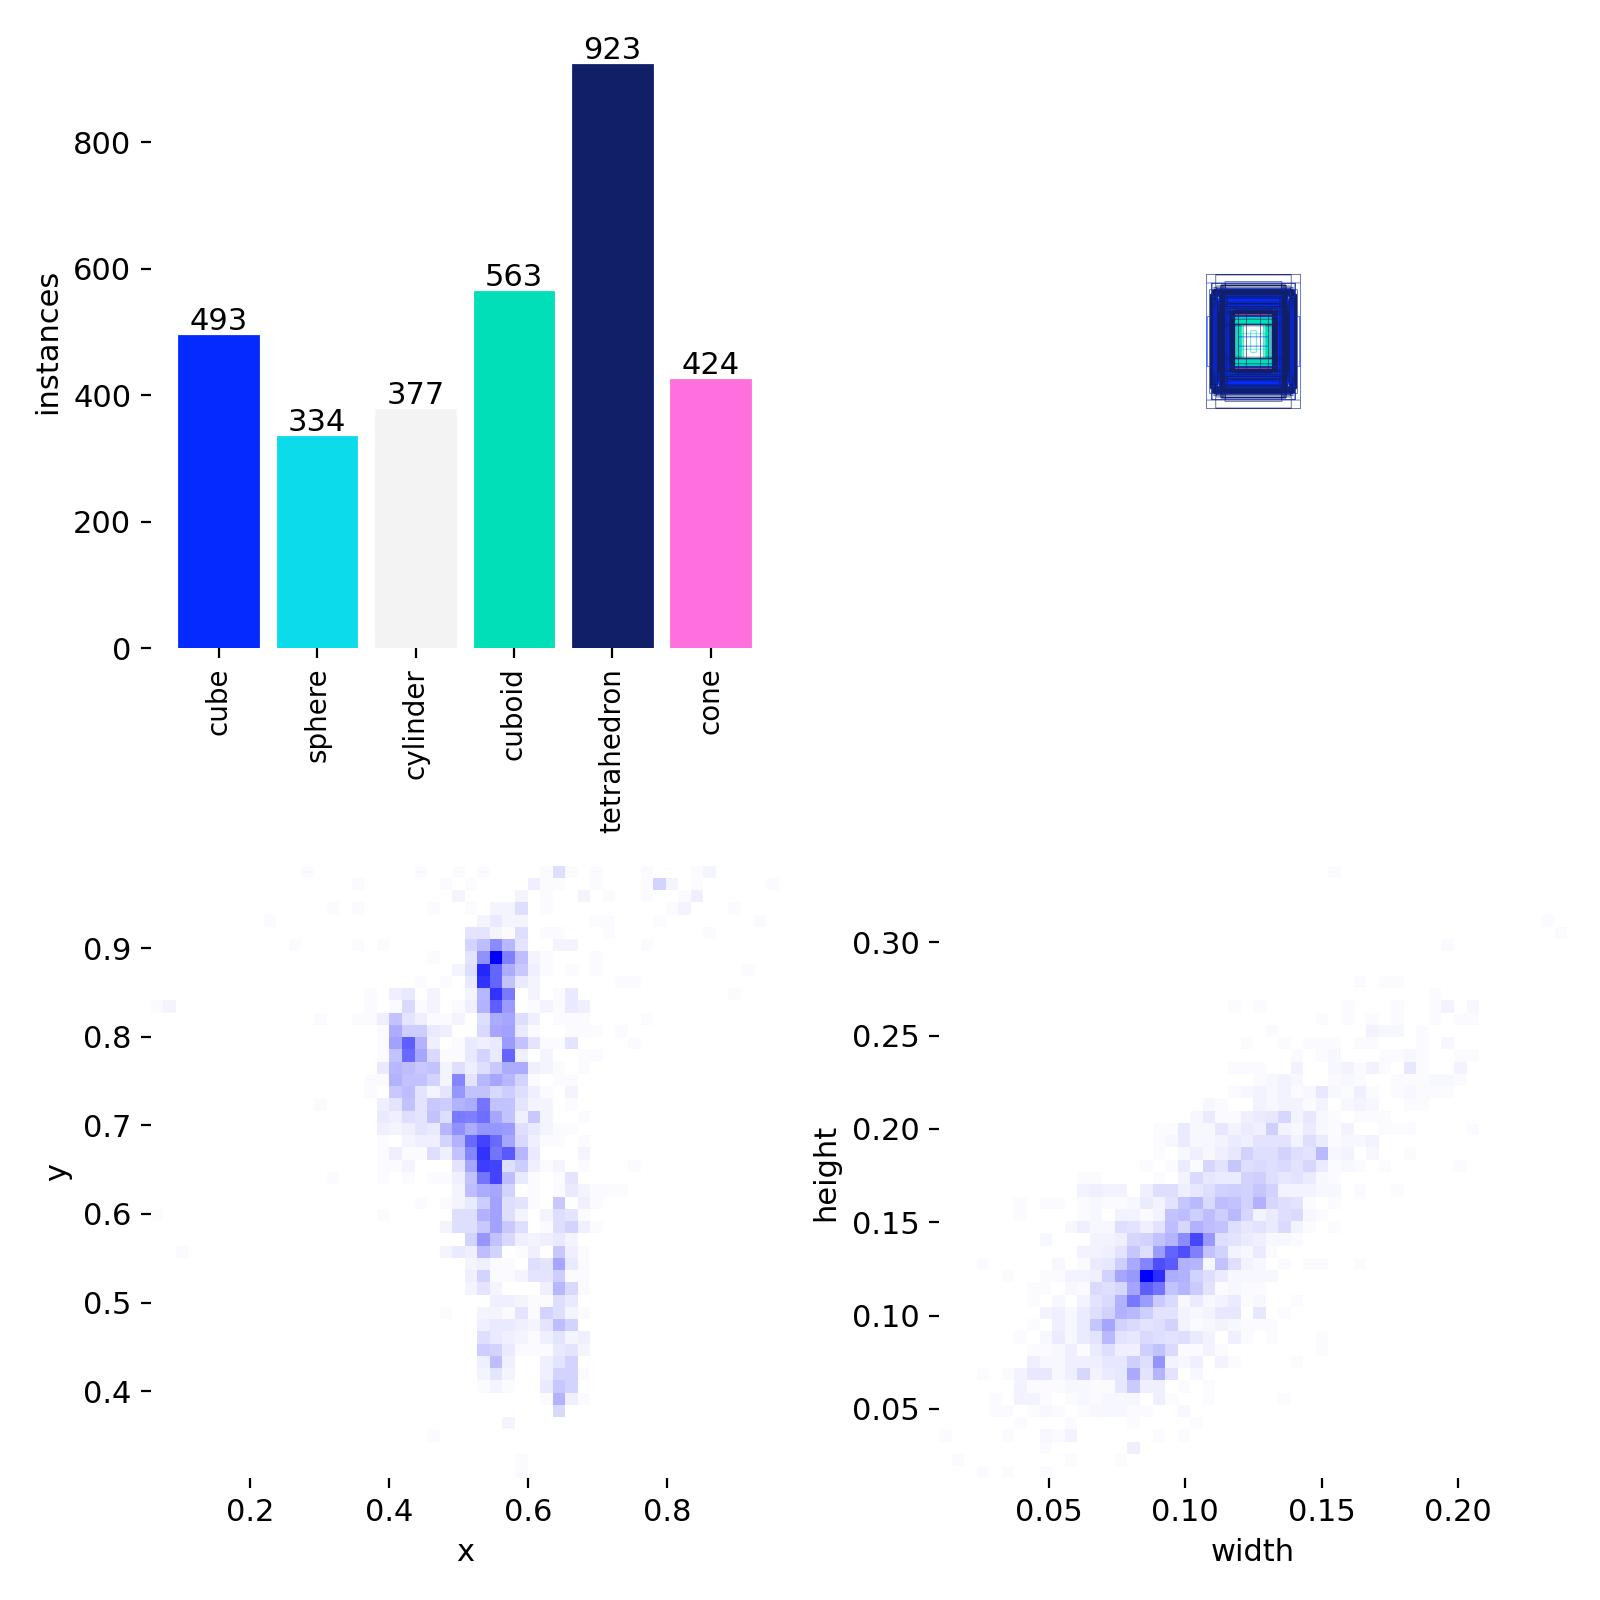
\includegraphics[width=0.8\textwidth]{./graf/labels.jpg}
    \caption{Rozkład klas oraz położenia ramek ograniczających w zbiorze treningowym.}
    \label{fig:dataset_labels}
\end{figure}

\subsection{Proces pozyskiwania i oznaczania danych}

Pierwszym etapem przygotowania zbioru danych było nagranie materiałów wideo zawierających wspomniane wcześniej widoki osoby manipulującej bryłami. Zarejestrowano je przy pomocy nieruchomego urządzenia mobilnego Samsung Galaxy S25 w rozdzielczości $1920\times1440$ i 30 klatkach na sekundę. Zostały one zrealizowane w różnych warunkach oświetleniowych z wykorzystaniem światła dziennego i sztucznego, z różnymi osobami i w różnych ubraniach. Na każdym nagraniu osoba manipuluje każdą z przygotowanych brył sposób odpowiadający przewidywanemu scenariuszowi użycia systemu. Ostatecznie nagrano 9 filmów o łącznej długości 14 minut i 16 sekund. Następnie, korzystając z przygotowanego skryptu (por.~\ref{ssec:extractor}), z wszystkich nagrań wyekstrahowano 4666 obrazów w formacie JPEG.

W następnym kroku obrazy należało oznaczyć, czyli przygotować adnotacje obiektów, które się na nich znajdują. Do tego zadania wykorzystano narzędzie \texttt{CVAT} \cite{bib:cvat} rozwijane przez firmę cvat.ai corporation. Zostało ono wybrane ze względu na możliwość pracy w przeglądarce internetowej, a także półautomatyczne oznaczanie obiektów korzystając z wcześniej wytrenowanego modelu detekcji. Niestety, w trakcie oznaczania napotkano problemy z uruchomieniem modelu w narzędziu, co skutkowało koniecznością ręcznego oznaczania wszystkich obiektów i rezygnacji z rozszerzenia zbioru o dodatkowe obrazy. Podczas pracy z narzędziem korzystano również z serwisu Amazon S3 do przechowywania danych w chmurze. Dzięki niemu nie zaistniała konieczność przesyłania dużych ilości danych pomiędzy wykorzystywanymi platformami.

\subsection{Podział danych na zbiory treningowy, walidacyjny i testowy}

Po oznaczeniu danych należało je podzielić na zbiory treningowy, walidacyjny i testowy. Wykonano ręczny podział danych tak, aby obrazy z pojedynczego nagrania nie były rozdzielone pomiędzy różne zbiory. Zadbano równocześnie, aby zbiór treningowy zawierał zróżnicowane obrazy, a zbiory walidacyjny i testowy zawierały wszystkie klasy oraz możliwie zróżnicowane przykłady scen. Nagrania, z których obrazy znalazły się w zbiorach treningowym i walidacyjnym zostały zarejestrowane pojedynczego dnia, a nagrania dla zbioru testowego zostały zarejestrowane kilka dni później. Ostateczny udział obrazów w pełnym zbiorze danych wynosił $81\%$ dla zbioru treningowego, $8,7\%$ dla zbioru walidacyjnego i $10,2\%$ dla zbioru testowego. Zrezygnowano z wykorzystania skryptu \texttt{split\_dataset.py} do podziału danych, aby nie mieszać obrazów, a tym samym wykluczyć możliwość rozpoznania obiektów na podstawie wyglądu sceny. Szczegółowy udział filmów w poszczególnych zbiorach przedstawiono w tabeli~\ref{tab:video_split}.

\begin{table}[ht]
    \caption{Podział nagrań wideo pomiędzy zbiory treningowy, walidacyjny i testowy.}
    \label{tab:video_split}
    \begin{tabularx}{\textwidth}{X|llll}
        \toprule
        \textbf{Data nagrania} &
        \makecell[tl]{\textbf{Długość nagrania} \\mm:ss} &
        \makecell[tl]{\textbf{Liczba}           \\\textbf{obrazów}} &
        \textbf{Zbiór}         &
        \textbf{Udział}                         \\
        \midrule
        \makecell[tl]{13-05-2026                \\12:39} & 04:07 & 1481 & treningowy & \makecell[tl]{całościowy: $31,7\%$\\w zbiorze: $39,2\%$} \\
        \makecell[tl]{13-05-2026                \\12:45} & 02:21 & 843 & treningowy & \makecell[tl]{całościowy: $18,1\%$\\w zbiorze: $22,3\%$} \\
        \makecell[tl]{13-05-2026                \\12:50} & 01:37 & 581 & treningowy & \makecell[tl]{całościowy: $12,5\%$\\w zbiorze: $15,4\%$} \\
        \makecell[tl]{13-05-2026                \\12:53} & 01:22 & 493 & treningowy & \makecell[tl]{całościowy: $10,6\%$\\w zbiorze: $13,0\%$} \\
        \makecell[tl]{13-05-2026                \\12:58} & 01:04 & 384 & treningowy & \makecell[tl]{całościowy: $8,2\%$\\w zbiorze: $10,2\%$} \\
        \makecell[tl]{13-05-2026                \\13:02} & 01:08 & 407 & walidacyjny & \makecell[tl]{całościowy: $8,7\%$\\w zbiorze: $100\%$} \\
        \makecell[tl]{19-05-2026                \\14:03} & 0:54 & 164 & testowy & \makecell[tl]{całościowy: $3,5\%$\\w zbiorze: $34,4\%$} \\
        \makecell[tl]{19-05-2026                \\14:06} & 0:54 & 164 & testowy & \makecell[tl]{całościowy: $3,5\%$\\w zbiorze: $34,4\%$} \\
        \makecell[tl]{19-05-2026                \\14:10} & 0:49 & 149 & testowy & \makecell[tl]{całościowy: $3,2\%$\\w zbiorze: $31,2\%$} \\
        \bottomrule
    \end{tabularx}
\end{table}

Przeznaczenie poszczególnych zbiorów danych jest zgodne z przyjętymi w literaturze standardami oraz nie występuje nakładanie się ich zastosowań. Zbiór treningowy służy wyłącznie do trenowania modeli, zbiór walidacyjny do oceny jakości modeli w trakcie treningu, a zbiór testowy jest używany wyłącznie do oceny jakości modeli po zakończeniu treningu.

\subsection{Warianty danych wejściowych}

Podstawowym wariantem danych wejściowych jest obraz kolorowy w przestrzeni barw RGB. Stanowi on punkt odniesienia dla wszystkich eksperymentów.

Aby sprawdzić eksperymentalnie wpływ koloru na jakość detekcji, postanowiono przetestować zdolność modeli na danych wejściowych w dwóch wariantach: kolorowym (RGB) oraz w odcieniach szarości (grayscale). Konwersja na odcienie szarości została wykonana obliczając wartość ważonej luminancji z wykorzystaniem wzoru:
\begin{equation}
    Y = 0,299 \cdot R + 0,587 \cdot G + 0,114 \cdot B.
\end{equation}
Taki dobór wag najlepiej odzwierciedla wpływ poszczególnych kanałów na postrzeganą jasność obrazu przez ludzkie oko. Następnie wartość luminancji została powielona na wszystkie trzy kanały, aby zachować zgodność z oczekiwanym przez modele wejściem.

Zastosowanie w tym miejscu średniej wartości kolorów:
\begin{equation}
    Y = \frac{R + G + B}{3}
\end{equation}
nie zostało uznane za właściwe, ponieważ eksperyment ma na celu sprawdzenie, czy usunięcie informacji o barwie będzie miało wpływ na jakość detekcji, a średnia wartość kolorów nie odzwierciedla rzeczywistego wpływu poszczególnych kolorów na postrzeganą jasność obrazu.

Repozytorium z projektem zawiera również filtr Sobela, jednakże nie został on wykorzystany w eksperymentach ponieważ oczekujemy, że model będzie w stanie samodzielnie wyznaczyć krawędzie obiektów. Użycie klasycznego, deterministycznego operatora detekcji krawędzi skutkuje zatraceniem informacji o teksturze i rozkładzie jasności w obrębie obiektów. Ich utrata może skutkować obniżeniem jakości detekcji, szczególnie w przypadku obiektów, które nie mają wyraźnych krawędzi, np. kuli.

Porównanie obrazów w wariancie kolorowym z obrazami na których zastosowano opisane filtry przedstawiono na rysunku~\ref{fig:dataset_variants}.

\begin{figure}
    \centering
    \begin{subfigure}[b]{0.45\textwidth}
        \centering
        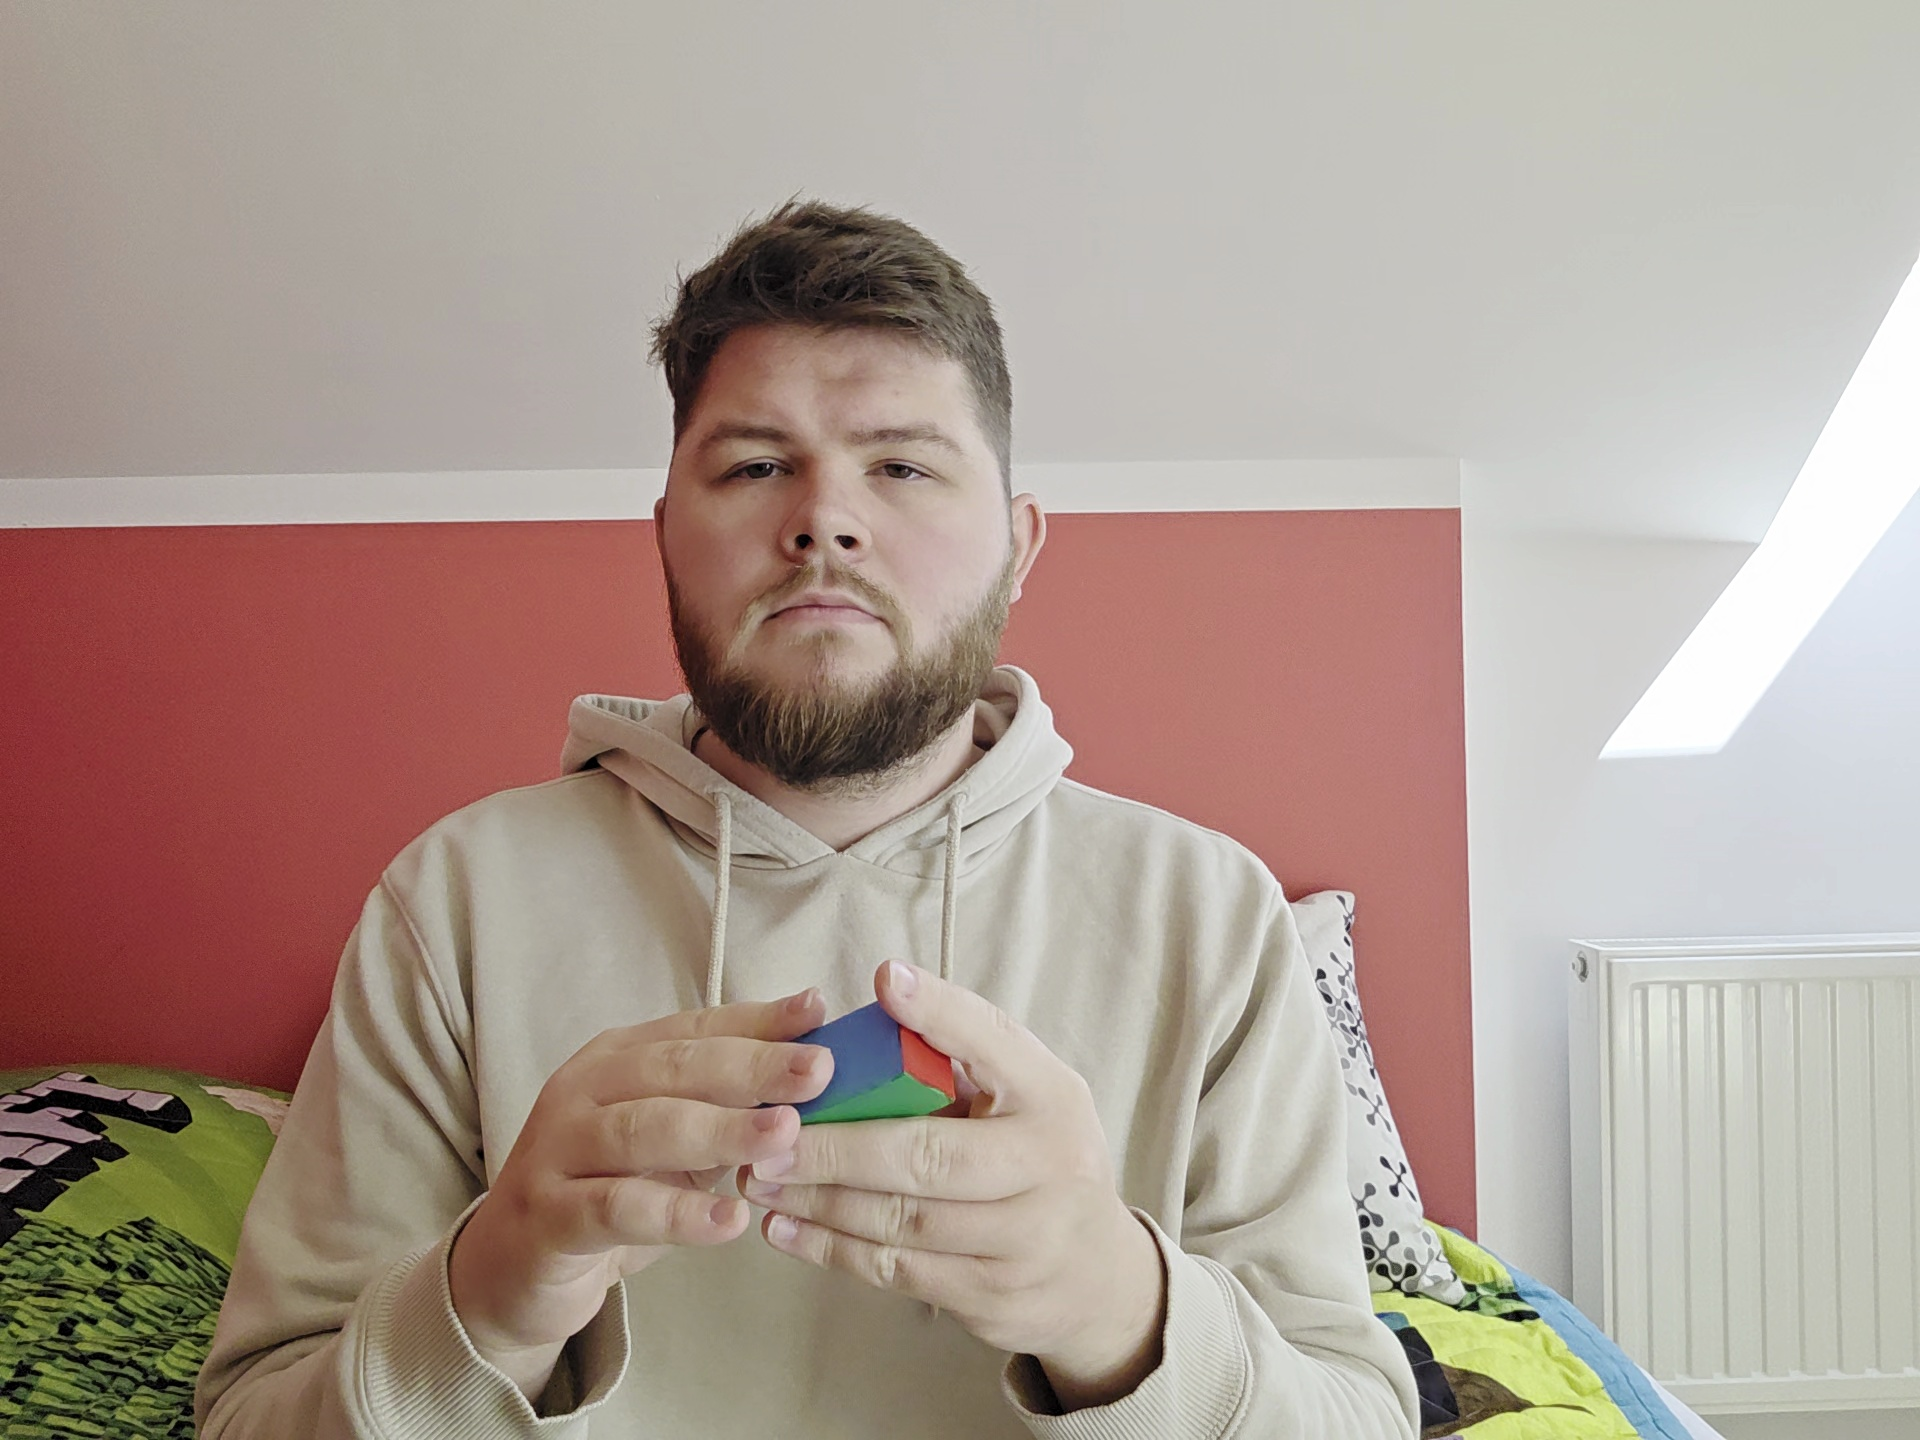
\includegraphics[width=\textwidth]{./graf/variants/frame_242_rgb.jpeg}
        \caption{Wariant kolorowy.}
        \label{fig:dataset_variants_rgb}
    \end{subfigure}
    \begin{subfigure}[b]{0.45\textwidth}
        \centering
        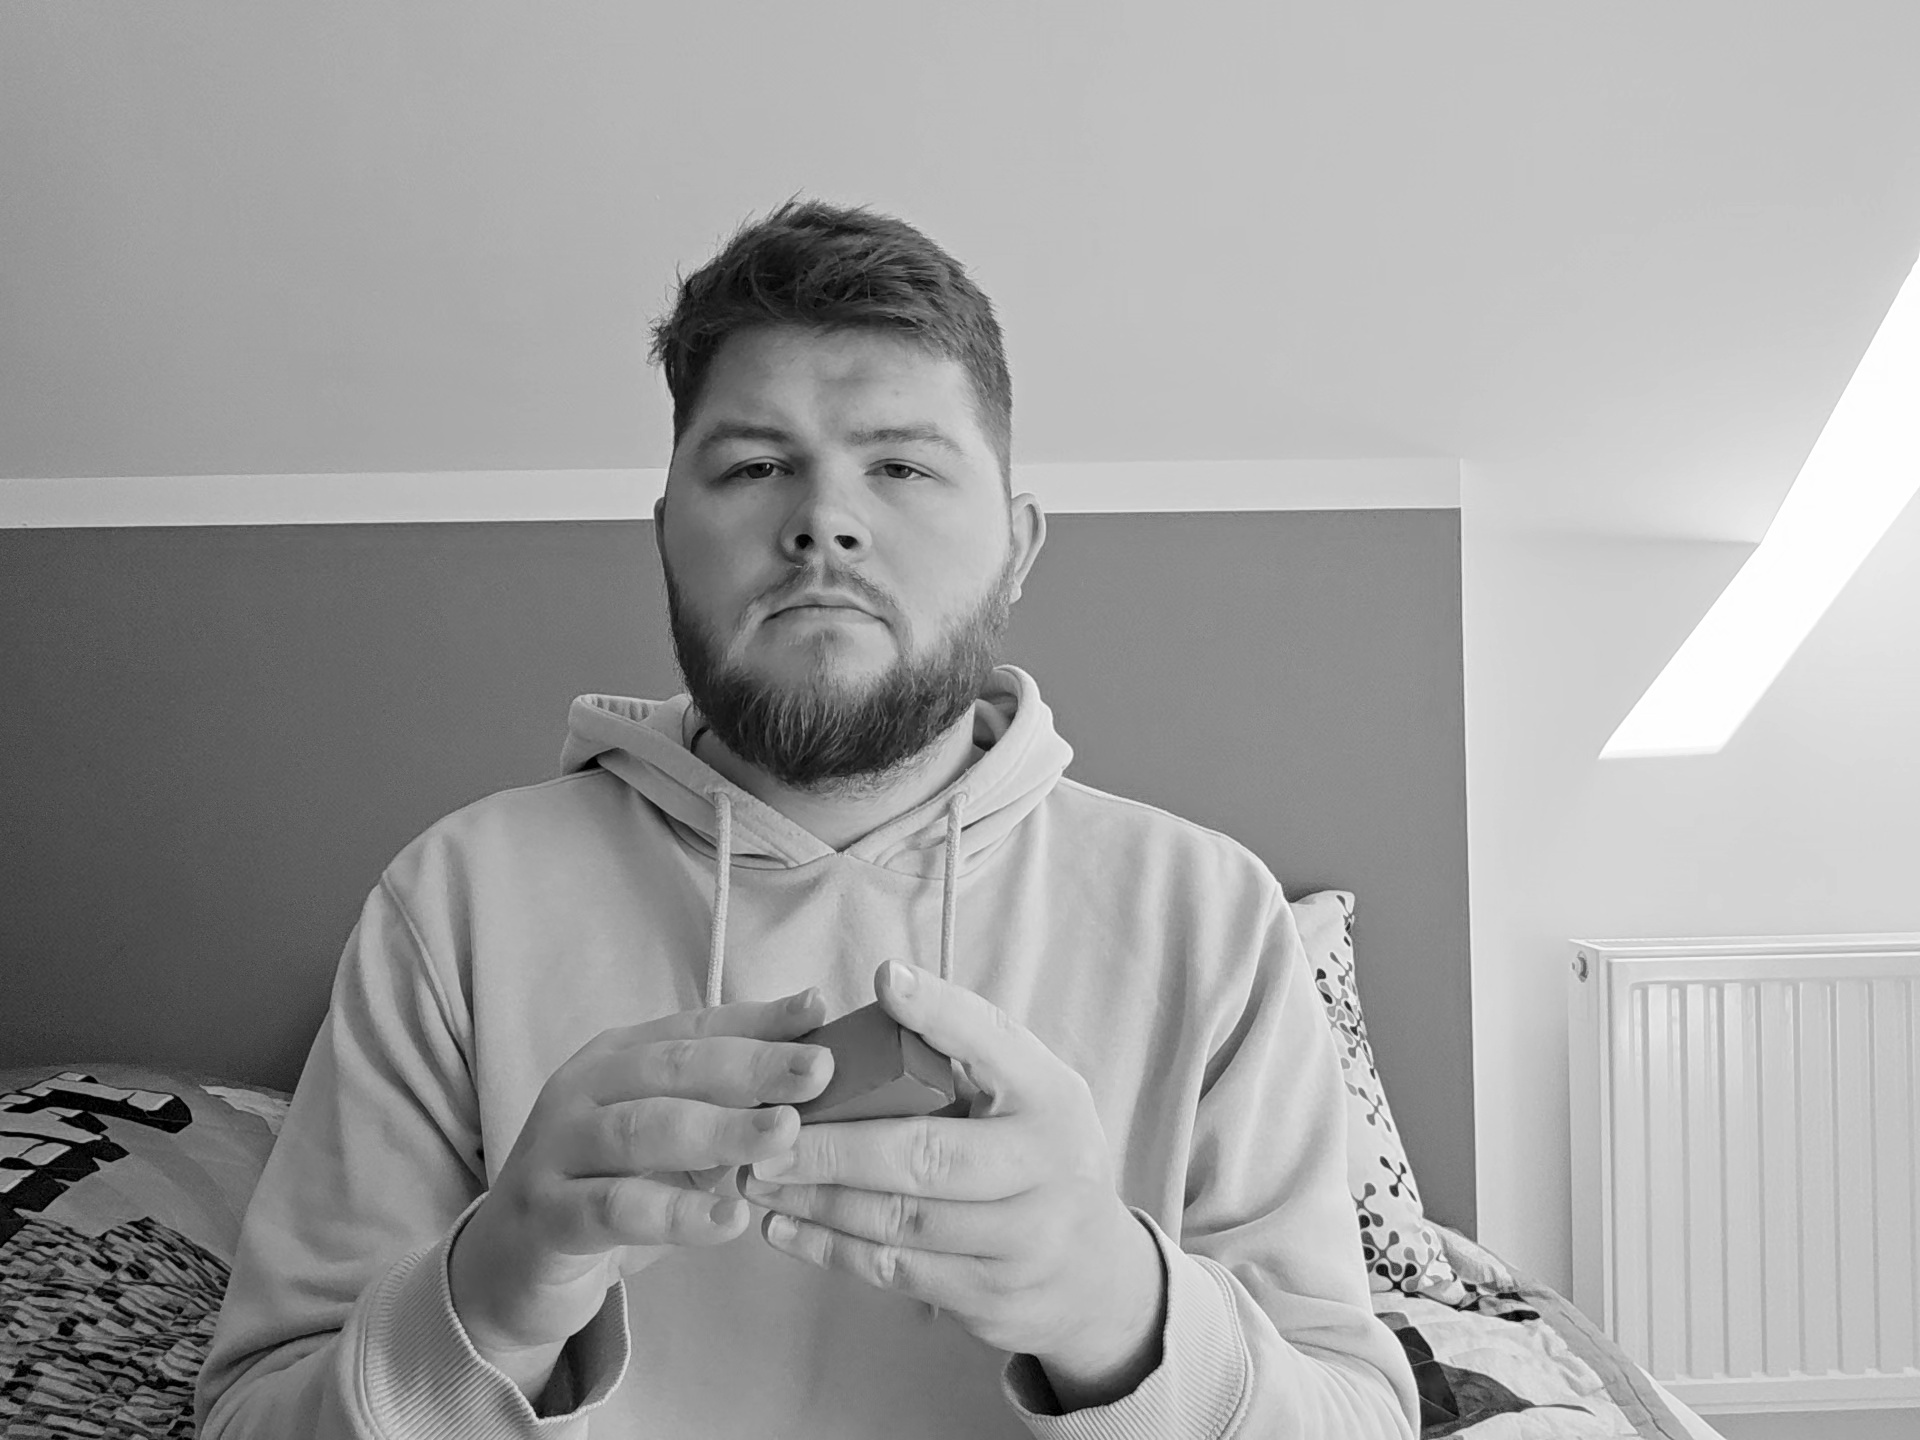
\includegraphics[width=\textwidth]{./graf/variants/frame_242_grayscale.jpeg}
        \caption{Wariant w odcieniach szarości.}
        \label{fig:dataset_variants_grayscale}
    \end{subfigure}
    \caption{Warianty danych wejściowych.}
    \label{fig:dataset_variants}
\end{figure}

\section{Metodyka eksperymentalna}

Poprawne przeprowadzenie badań wymaga ustalenia kryteriów oceny poszczególnych modeli, a także przyjęcia procedury eksperymentalnej, która umożliwi porównanie jakości detekcji pomiędzy nimi. W tym celu należy ustalić metryki oceny, a także parametry treningu modeli.

\subsection{Konfiguracja treningu modeli}

Skrypt treningowy \texttt{train.py} umożliwia konfigurację wielu parametrów treningu modelu. W eksperymentach nie wykorzystano wszystkich dostępnych opcji, a jedynie te, które uwydatnią różnice w jakości detekcji pomiędzy poszczególnymi wariantami modeli. Podczas treningu zmieniano trzy elementy konfiguracji:

\begin{itemize}
    \item \textbf{model} -- wariant modelu: YOLO26n, YOLO26s,
    \item \textbf{zbiór danych} -- warianty zbioru danych: RGB, odcienie szarości,
    \item \textbf{rozmiar obrazu} -- rozdzielczość obrazu wejściowego: $640$, $1024$.
          % \item \textbf{urządzenie} -- urządzenie, na którym przeprowadzono trening: NVIDIA A100, NVIDIA L40S, NVIDIA RTX 4060
          % \item \textbf{system operacyjny} -- system operacyjny, na którym przeprowadzono trening: Ubuntu 22.04, Windows 11.
\end{itemize}
Łącznie wytrenowano 7 modeli, które pozwoliły na przeprowadzenie eksperymentów i porównanie jakości detekcji pomiędzy nimi.

Urządzenia wykorzystane do treningu były wybierane według dostępności w danym momencie, a nie według ich wydajności. Trening na karcie graficznej NVIDIA RTX 4060 był wykonywany na lokalnym komputerze z systemem Windows~11, a treningi na pozostałych kartach odbywały się w chmurze za pomocą platformy RunPod z systemem Ubuntu~22.04. Urządzenie obliczeniowe i system operacyjny nie są zmiennymi badanymi,a ich wpływ na jakość uzyskanych modeli nie jest przedmiotem badań.

Augmentacja danych została włączona w celu zwiększenia różnorodności danych treningowych i poprawy zdolności generalizacji modeli. Wykorzystano w tym celu wbudowane w narzędzie Ultralytics YOLO mechanizmy augmentacji pozostawiając ich parametry domyślne. Obejmują one modyfikacje składowych HSV, translację, skalowanie, odbicia poziome oraz augmentację mozaikową.

Trening modeli był prowadzony do momentu braku poprawy kryterium walidacyjnego przez 50 kolejnych epok (ang. \english{early stop}). Po tym czasie trening był przerywany i uznawano, że model osiągnął swoje plateau i dalszy trening nie przyniesie znaczącej poprawy jakości detekcji. Przyjęta wartość parametru \texttt{patience} jest kompromisem pomiędzy przedwczesnym zakończeniem treningu a niepotrzebnym wydłużeniem jego czasu \cite{bib:Prechelt1998}.

Każdy trening uruchomiony został z ustawieniem ziarna generatora liczb pseudolosowych na wartość 42. Zwiększa to powtarzalność wyników oraz ułatwia odtworzenie eksperymentów w przyszłości. Wartość ta została wybrana ze względu na jej popularność w literaturze i kulturze komputerowej\footnote{Wartość 42 jest nawiązaniem do powieści Douglasa Adamsa \textit{Autostopem przez Galaktykę}, gdzie stanowi odpowiedź na  "Wielkie Pytanie o Życie, Wszechświat i całą resztę"}.

Do treningu wykorzystano następujące wersje bibliotek i narzędzi:
\begin{itemize}
    \item \textbf{Python} -- 3.11.11,
    \item \textbf{Ultralytics} -- 8.4.63,
    \item \textbf{PyTorch} -- 2.12.0,
    \item \textbf{matplotlib} -- 3.10.9,
    \item \textbf{opencv-python} -- 4.13.0.92,
    \item \textbf{CUDA} -- 13.2.
\end{itemize}

\subsection{Metryki oceny}

Do oceny poszczególnych modeli wykorzystano metryki zwracane przez bibliotekę Ultralytics: precision, recall, $mAP50$, $mAP50\text{-}95$ oraz macierze pomyłek. Dodatkowo obliczano wartość $F1$-score dla najlepszego modelu w każdym eksperymencie. Szczegółowe opisy każdej z użytych metryk znajdują się w sekcji~\ref{s:metryki}.

Dokładne przebiegi każdego treningu znajdują się w pliku \texttt{results.csv}, a porównanie najlepszej epoki treningu z ostatnią przedstawia plik \texttt{run\_stats.json}.

Najważniejszą z używanych metryk jest $mAP50\text{-}95$, ponieważ uwzględnia ona jakość detekcji dla wielu progów IoU i pozwala na ocenę zarówno jakości lokalizacji, jak i klasyfikacji obiektów \cite{bib:ultralytics_yolo_metrics}. Jako metryka pomocnicza użyto siostrzaną metrykę $mAP50$, która jest łatwiejsza do interpretacji i ukazuje skuteczność detekcji przy mniej rygorystycznych kryteriach. Kolejno, metryki precision i recall umożliwiają ocenę jakości detekcji w kontekście liczby wykrytych obiektów, a ich średnia harmoniczna $F1$-score opisuje kompromis pomiędzy nimi. Niezwykle przydatne okazują się również macierze pomyłek, na których podstawie można określić, które klasy są najtrudniejsze do wykrycia i które są najczęściej mylone z innymi.

Do porównania należy wykorzystać metryki, które zostały wyznaczone na zbiorze testowym, a nie na zbiorze walidacyjnym. Zbiór walidacyjny służy wyłącznie do oceny jakości predykcji podczas treningu do wyznaczenia najlepszej epoki treningu, podczas gdy zbiór testowy jest wykorzystywany do końcowej oceny modelu. Ważne jest również, aby przy każdym eksperymencie używać dokładnie tego samego zbioru testowego, aby zachować miarodajne porównanie poszczególnych modeli. Wyniki tej oceny stanowią podstawę do porównania modeli przedstawionego w rozdziale~\ref{c:badania}.

Oprócz metryk jakości detekcji przy końcowym porównaniu modeli uwzględniono liczbę ich parametrów, koszt obliczeniowy wyrażony w GFLOPs, rozmiar pliku modelu oraz czas inferencji i wynikającą z niego liczbę przetwarzanych klatek na sekundę. Wartości te zebrano w dwóch niezależnych seriach pomiarowych na pojedynczym urządzeniu.

Nie porównywano pełnego czasu odpowiedzi ponieważ jest on silnie zależny od używanego urządzenia obliczeniowego, przepustowości sieci oraz obciążenia systemu operacyjnego. Każdy przypadek wdrożenia systemu należy oceniać indywidualnie, na podstawie wyników eksperymentów przeprowadzonych na docelowym sprzęcie i w docelowych warunkach pracy.

\subsection{Procedura eksperymentalna}
\label{ssec:procedure}

Aby móc dokonać porównania jakości detekcji pomiędzy poszczególnymi wariantami modeli należy podzielić je na eksperymenty. Każdy z nich polegał na wytrenowaniu kilku, porównywalnych modeli, które różniły się pojedynczym parametrem. Wykonano następujące eksperymenty:

\begin{enumerate}[label=\textbf{Eksperyment \Alph*:}, leftmargin=*, align=left]
    \item Porównanie jakości detekcji pomiędzy rozmiarami modelu YOLO26 \texttt{n} i \texttt{s} dla danych wejściowych w wariancie kolorowym. Pozwoli to ocenić wpływ skali modelu i ilość jego parametrów na jakość detekcji.
    \item Porównanie jakości detekcji pomiędzy wariantami z różnymi rozdzielczościami obrazu wejściowego: $640$ oraz $1024$. Pozwoli on ocenic wpływ rozdzielczości obrazu na jakość detekcji.
    \item Porównanie jakości detekcji pomiędzy wariantami danych: kolorowym i w odcieniach szarości. Pozwoli to ocenić, czy usunięcie informacji o barwie wpływa na jakość detekcji i czy model jest w stanie skutecznie rozpoznać obiekty bez wykorzystania informacji o kolorze.
\end{enumerate}

Przedstawione eksperymenty pozwalają ocenić, czy możliwe jest skuteczne rozpoznawanie trzymanych obiektów trójwymiarowych bez informacji o kolorze, a także czy możliwe jest uzyskanie zadowalających wyników przy użyciu modeli o mniejszej liczbie parametrów. Wyniki poszczególnych eksperymentów zostały przedstawione w rozdziale~\ref{c:badania}. % Zbiór danych i metodyka badań

% TODO
\chapter{Wyniki badań i~ich analiza}
\label{c:badania}

Wyniki, jakie otrzymano z~przeprowadzonych eksperymentów pozwalają określić, czy badany problem rozpoznawania brył może zostać rozwiązany z~użyciem metod uczenia głębokiego. Niniejszy rozdział prezentuje uzyskane wyniki oraz ich analizę. Przeprowadzono w~nim również analizę najczęstszych błędów modeli i~wysnuto wnioski dlaczego~\nobreakdash{zachodzą}.

Do przeprowadzenia eksperymentów wytrenowano siedem sieci o~architekturze YOLO, wykorzystując ten sam zbiór danych, korzystając z~procesorów graficznych firmy NVIDIA. W~części eksperymentów obrazy przed treningiem przekształcono do odcieni szarości zgodnie z~procedurą opisaną w~\ref{ssec:filtry}. Macierz wariantów modeli została przedstawiona w~tabeli~\ref{tab:exp_matrix}. Taka liczba modeli pozwala na przeprowadzenie eksperymentów założonych w~sekcji \ref{ssec:procedure}.

\begin{table}[ht]
    \centering
    \caption{Macierz modeli wytrenowanych w~ramach badań.}
    \label{tab:exp_matrix}
    \begin{tabular}{l|cccc}
        \toprule
        \textbf{Model} & \textbf{RGB 640} & \textbf{RGB 1024} & \textbf{grayscale 640} & \textbf{grayscale 1024} \\
        \midrule
        YOLO26n        & \checkmark       & \checkmark        & \checkmark             & \checkmark              \\
        YOLO26s        & \checkmark       & \checkmark        & \checkmark             &                         \\
        \bottomrule
    \end{tabular}
\end{table}

\section{Zestawienie wyników treningów} % 6.1

Każdy z~wytrenowanych modeli został oceniony pod kątem jakości detekcji na zbiorze testowym. Do oceny jakości detekcji za każdym razem wykorzystano model, który w~trakcie uczenia osiągnął najlepsze wyniki na zbiorze walidacyjnym. Kryterium wyboru najlepszego modelu była wartość $mAP50\text{-}95$. Po przeprowadzeniu treningu każdy z~modeli został oceniony na zbiorze testowym, a~wyniki zostały zestawione w~tabeli~\ref{tab:results}.

\begin{table}[ht]
    \centering
    \footnotesize
    \caption{Zestawienie wyników detekcji modeli na zbiorze testowym.}
    \label{tab:results}
    \begin{tabular}{l|ccccccc}
        \toprule
        \textbf{ID}              & $E_1$    & $E_2$    & $E_3$   & $E_4$   & $E_5$     & $E_6$     & $E_7$     \\
        \midrule
        \textbf{Model}           & YOLO26n  & YOLO26s  & YOLO26n & YOLO26s & YOLO26n   & YOLO26s   & YOLO26n   \\
        \textbf{Dane}            & RGB      & RGB      & RGB     & RGB     & grayscale & grayscale & grayscale \\
        \textbf{Rozmiar obrazu}  & 640      & 640      & 1024    & 1024    & 640       & 640       & 1024      \\
        \textbf{Ostatnia epoka}  & 190      & 108      & 211     & 114     & 203       & 280       & 230       \\
        \textbf{Najlepsza epoka} & 140      & 60       & 161     & 64      & 153       & 230       & 180       \\
        \midrule
        \textbf{Precision}       & 0.714    & 0.701    & 0.794   & 0.846   & 0.591     & 0.630     & 0.649     \\
        \textbf{Recall}          & 0.678    & 0.760    & 0.825   & 0.736   & 0.475     & 0.601     & 0.601     \\
        $mAP50$                  & 0.716    & 0.786    & 0.862   & 0.844   & 0.488     & 0.560     & 0.621     \\
        $mAP50\text{-}95$        & 0.599    & 0.641    & 0.719   & 0.729   & 0.360     & 0.449     & 0.495     \\
        \textbf{$F1$-score}      & 0.696    & 0.730    & 0.809   & 0.787   & 0.526     & 0.615     & 0.624     \\
        \midrule
        \textbf{GPU}             & RTX 4060 & RTX 4060 & L40S    & L40S    & A100      & A100      & A100      \\
        \bottomrule
    \end{tabular}
\end{table}

Prawie każdy z~treningów zakończył się jego wcześniejszym zatrzymaniem, co oznacza, że w~trakcie uczenia model osiągnął wartość $mAP50\text{-}95$ na zbiorze walidacyjnym, która nie uległa poprawie przez 50 kolejnych epok. Uczenie modelu $E_2$ zakończono po 48 epokach bez poprawy wartości ze względu na ograniczenia czasowe dostępu do jednostki obliczeniowej i~nie podjęto decyzji o~kontynuacji treningu. Trening wariantu \texttt{s} na obrazach kolorowych w~obu przypadkach ($E_2$, $E_4$) potrzebował mniejszej liczby epok do osiągnięcia najlepszej wartości kryterium walidacyjnego niż wariant \texttt{n} ($E_1$, $E_3$).

Większość treningów modeli miała stabilny przebieg, charakteryzujący się szybkim wzrostem wartości metryk mAP, a~następnie ich wypłaszczenie. Jest to typowe zachowanie w~procesie uczenia modeli YOLO, które w~początkowej fazie szybko dopasowują się do danych treningowych, a~następnie optymalizują wagi w~celu poprawy jakości detekcji. Przebieg treningu modelu $E_1$ wraz ze zmianami wartości jego metryk został przedstawiony na rysunku~\ref{fig:training_curve}. Możemy na nim zaobserwować, że wartości funkcji straty dla zbioru uczącego systematycznie maleją, co świadczy o~tym, że model uczy się coraz lepiej dopasowywać do danych treningowych. Podobne tendencje, choć nie tak wyraźne, obserwujemy w~przypadku wartości funkcji straty dla zbioru walidacyjnego. Jednocześnie wartości metryk jakości detekcji szybko rosną świadcząc o~tym, że model coraz lepiej dopasowuje etykiety do obiektów na obrazach.

\begin{figure}[htbp]
    \centering
    \begin{subfigure}{\textwidth}
        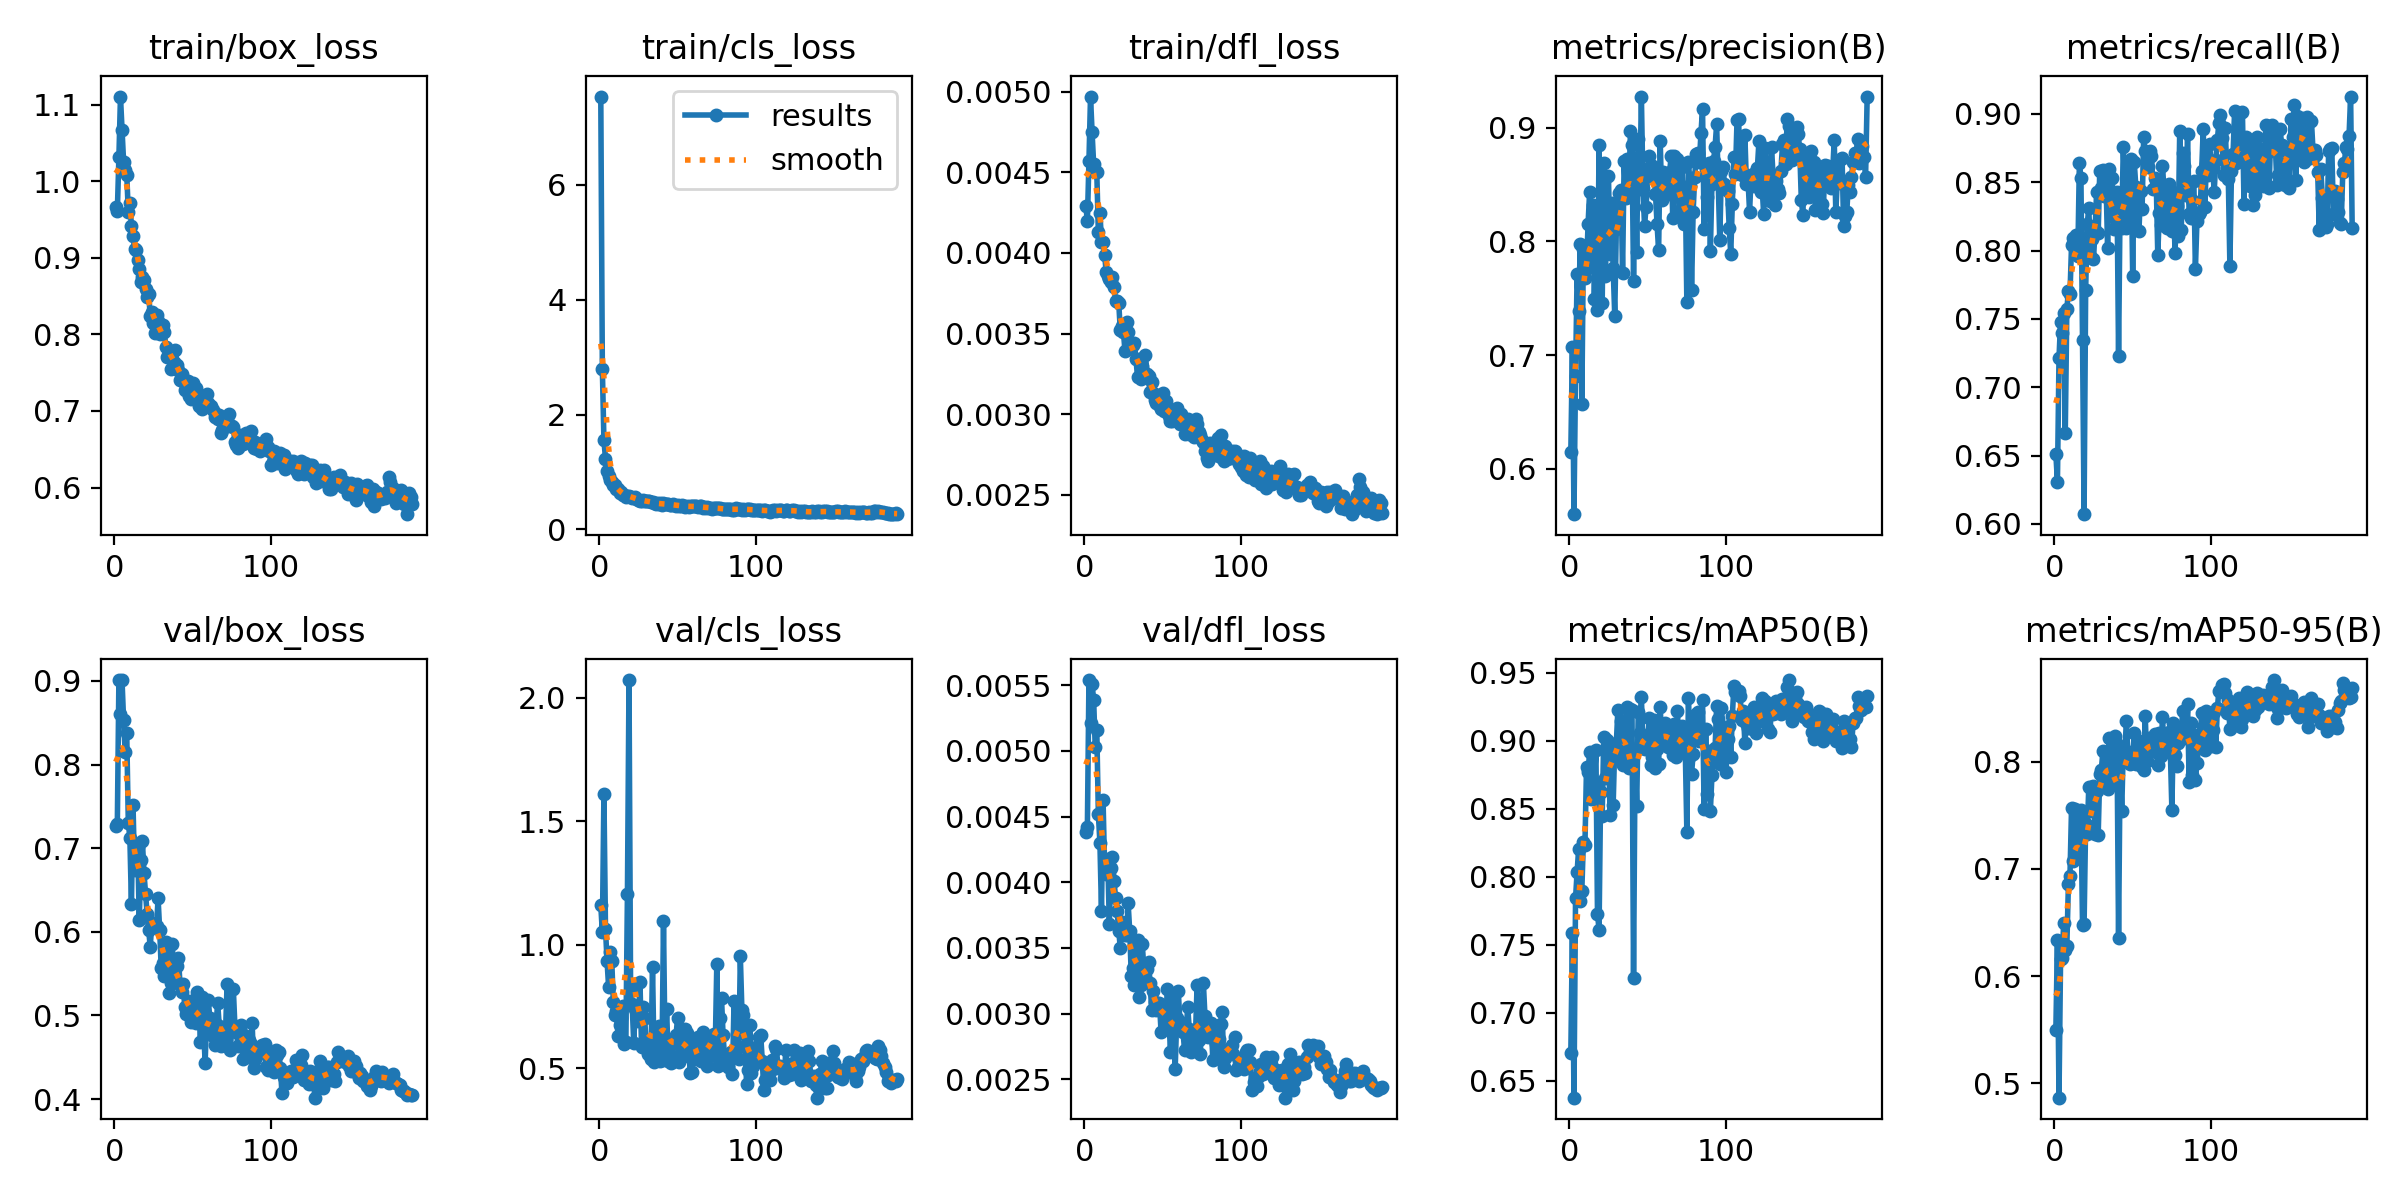
\includegraphics[width=\textwidth]{./graf/yolo26n_640_rgb_results.png}
        \caption{Przebieg treningu wariantu $E_1$.}
        \label{fig:training_curve}
    \end{subfigure}

    \vspace{1cm}

    \begin{subfigure}{\textwidth}
        \includegraphics[width=\textwidth]{./graf/yolo26s_640_rgb_results.png}
        \caption{Przebieg treningu wariantu $E_2$.}
        \label{fig:training_curve_e2}
    \end{subfigure}
    \caption{Przebiegi treningu modeli YOLO26 na obrazach kolorowych o~rozdzielczości 640 pikseli.}
\end{figure}

Ciekawym przypadkiem jest trening modelu $E_2$, który osiągnął najlepszą wartość metryki w~60. epoce. Analiza przebiegu uczenia, ukazanego na rysunku~\ref{fig:training_curve_e2}, pokazuje, że w~trakcie treningu wystąpiło nagłe załamanie wartości metryk jakości detekcji. Pomimo systematycznego spadku wartości funkcji straty, od około połowy treningu funkcja straty na zbiorze walidacyjnym zaczęła wzrastać. W~końcowej fazie treningu widzimy jednak powrót do klasycznego przebiegu uczenia, co może skłaniać do przeprowadzenia dalszych badań nad tym przypadkiem. Obserwowany przebieg uzasadniałby ponowienie treningu modelu $E_2$ w~celu sprawdzenia, czy wzrost metryk walidacyjnych utrzymałby się w~kolejnych epokach.

\section{Wpływ skali modelu na jakość detekcji} % 6.2

Aby ocenić wpływ skali modelu na jakość detekcji, w~eksperymencie A~porównano modele YOLO26n i~YOLO26s. W~tym celu wykorzystano modele wytrenowane na obrazach kolorowych o~rozdzielczościach 640 ($E_1$, $E_2$) oraz 1024 pikseli ($E_3$, $E_4$). Wyniki zestawiono parami, tak aby w~każdym porównaniu jedyną zmienną była skala modelu. Wartości metryk dla poszczególnych porównań przedstawiono w~tabeli~\ref{tab:exp_a}.

\begin{table}[ht]
    \centering
    \caption{Porównanie jakości wariantów modeli YOLO26 n i~s w~eksperymencie A.}
    \label{tab:exp_a}
    \begin{tabular}{l|ccc|ccc}
        \toprule
        \multirow{2}{*}{\textbf{Metryka}}
         & \multicolumn{3}{c|}{\textbf{RGB 640}}
         & \multicolumn{3}{c}{\textbf{RGB 1024}}                           \\
        \cline{2-7}
         & YOLO26n                               & YOLO26s & Różnica (s-n)
         & YOLO26n                               & YOLO26s & Różnica (s-n) \\
        \midrule
        $mAP50$
         & 0.71595                               & 0.78551 & +0.06957
         & 0.86231                               & 0.84409 & -0.01823      \\

        $mAP50\text{-}95$
         & 0.59866                               & 0.64119 & +0.04253
         & 0.71856                               & 0.72932 & +0.01077      \\

        $F1$-score
         & 0.69568                               & 0.73041 & +0.03473
         & 0.80908                               & 0.78712 & -0.02195      \\
        \bottomrule
    \end{tabular}
\end{table}

Dla obrazów o~rozdzielczości 640 pikseli wyższą wartość analizowanych metryk osiągnął wariant \texttt{s}. Wartość $mAP50$ uległa poprawie o~$6,96$ p.p. (punktu procentowego), a~dla bardziej rygorystycznej $mAP50\text{-}95$ różnica wyniosła około $4,25$ p.p. Wartość wskaźnika $F1$-score również wzrosła, co wskazuje, że w~takiej konfiguracji większy model wykazuje się lepszą jakością detekcji na zbiorze testowym.

Inną zależność obserwujemy przy większych obrazach wejściowych o~rozdzielczości 1024 pikseli. Model YOLO26s uzyskał nieznacznie wyższą wartość $mAP50\text{-}95$, o~$1,08$ p.p. Jednocześnie, mniejszy wariant osiągnął wyższe wartości $mAP50$ i~wskaźnika $F1$-score. Oznacza to, że przy większym obrazie wejściowym wzrost skali modelu nie przekłada się bezpośrednio na poprawę jakości detekcji.

Porównanie obu rozdzielczości wskazuje, że wpływ zwiększenia skali modelu zależy od rozmiaru obrazu wejściowego. Dla mniejszych obrazów lepszą jakość detekcji wykazuje model YOLO26s. Przy obrazach o~rozdzielczości 1024 pikseli korzyść użycia większego modelu widoczna jest jedynie w~wartości metryki $mAP50\text{-}95$. Można więc zauważyć, że zwiększenie skali modelu ma większe znaczenie przy korzystaniu z~mniejszych obrazów wejściowych, natomiast przy większej ilości danych na wejściu przewaga większego wariantu ulega znacznemu ograniczeniu.

Wyniki eksperymentu A~nie wskazują więc na stałą przewagę jednego wariantu, a~raczej na zależność jakości detekcji od ilości informacji dostarczanych modelowi. YOLO26s przynosi znaczną poprawę dla mniejszych obrazów, lecz dla wariantu 1024 oba modele zachowują podobne właściwości detekcji. Ocena zasadności użycia większego wariantu modelu wymaga więc uwzględnienia również innych czynników, takich jak koszt obliczeniowy i~czas inferencji, które zostaną zestawione w~kolejnych sekcjach rozdziału.

\section{Wpływ rozdzielczości obrazu wejściowego na jakość detekcji} % 6.3

W~kolejnym eksperymencie badano wpływ rozmiaru wejściowego obrazu na jakość detekcji, porównując ze sobą modele trenowane na obrazach kolorowych z~parametrem \texttt{imgsz} ustawionym na 640 i~1024 piksele. Do porównania wykorzystano pary modeli o~tej samej skali, tak aby możliwe było wyizolowanie wpływu rozdzielczości obrazu wejściowego na jakość detekcji. Wyniki porównania zestawiono w~tabeli~\ref{tab:exp_b}.

Przykład wpływu rozdzielczości obrazu wejściowego przedstawiono na rysunku~\ref{fig:img_resize}. W~prezentowanym przypadku w~wariancie 640 bryła jest reprezentowana przez $11730$ pikseli, a~w~wariancie 1024 przez $29646$ pikseli. Stanowi to wzrost o~$2,53$ razy i~może wpływać na zdolność modelu do wykrywania obiektów, szczególnie w~przypadku mniejszych brył. Warto jednak zauważyć, że zwiększenie rozdzielczości obrazu wejściowego niesie za sobą również zwiększony koszt obliczeniowy oraz wydłużenie czasu inferencji.

\begin{table}[ht]
    \centering
    \caption{Porównanie jakości modeli dla rozmiarów obrazu wejściowego 640 i~1024 pikseli w~eksperymencie B.}
    \label{tab:exp_b}
    \begin{tabular}{l|ccc|ccc}
        \toprule
        \multirow{2}{*}{\textbf{Metryka}}
         & \multicolumn{3}{c|}{\textbf{YOLO26n}}
         & \multicolumn{3}{c}{\textbf{YOLO26s}}                       \\
        \cline{2-7}
         & 640                                   & 1024    & Różnica
         & 640                                   & 1024    & Różnica  \\
        \midrule
        $mAP50$
         & 0.71595                               & 0.86231 & +0.14636
         & 0.78551                               & 0.84409 & +0.05857 \\

        $mAP50\text{-}95$
         & 0.59866                               & 0.71856 & +0.11990
         & 0.64119                               & 0.72932 & +0.08813 \\

        $F1$-score
         & 0.69568                               & 0.80908 & +0.11340
         & 0.73041                               & 0.78712 & +0.05672 \\
        \bottomrule
    \end{tabular}
\end{table}

\begin{figure}[ht]
    \centering
    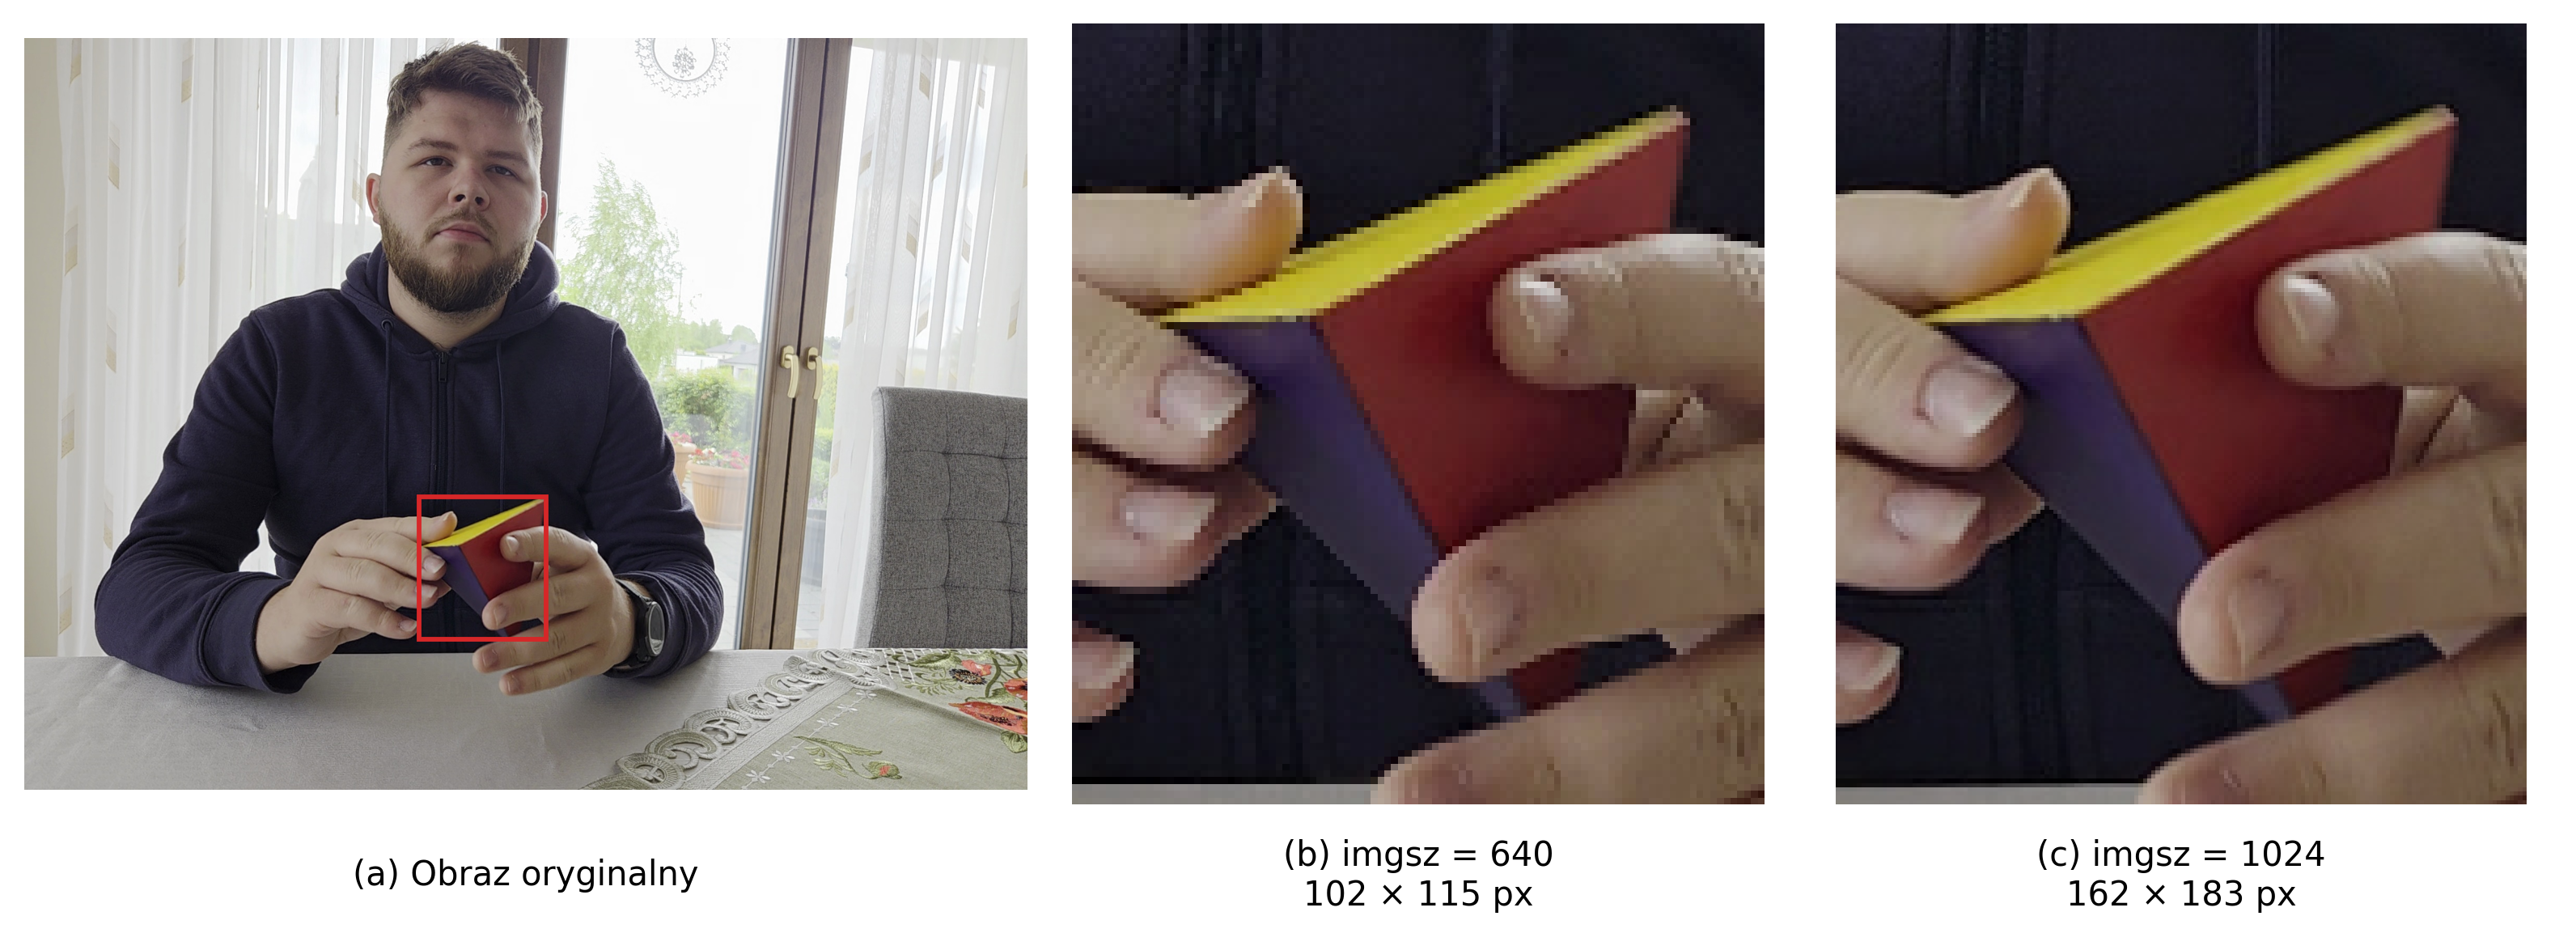
\includegraphics[width=\textwidth]{./graf/img_resize.png}
    \caption{Wizualizacja różnicy rozmiaru obiektu na obrazie w~zależności od rozdzielczości obrazu wejściowego.}
    \label{fig:img_resize}
\end{figure}

Zwiększenie rozdzielczości obrazu wejściowego przyniosło poprawę wszystkich analizowanych wartości metryk dla obu wariantów modeli. Największe zmiany można zauważyć w~przypadku YOLO26n. Wartość metryki $mAP50$ wzrosła o~$14,64$ p.p., a~$mAP50\text{-}95$ o~około $12$ p.p. Jednocześnie wskaźnik $F1$-score wzrósł o~$11,34$ p.p. Wyniki te wskazują na wyraźny wzrost jakości detekcji wraz z~zwiększeniem szczegółowości obrazu wejściowego poprzez zmianę jego rozdzielczości.

Poprawa występuje również dla wariantu \texttt{s}, jednak nie osiąga ona takiego poziomu jak w~przypadku YOLO26n. Zwiększenie rozmiaru wejścia do 1024 pikseli podniosło wartość $mAP50$ o~$5,86$ p.p., $mAP50\text{-}95$ o~$8,81$ p.p., a~$F1$-score o~$5,67$ p.p. W~przeciwieństwie do wariantu \texttt{n}, największy wzrost obserwuje się w~przypadku bardziej rygorystycznej metryki~$mAP50\text{-}95$.

Wyniki porównań pokazują, że rozmiar obrazu wejściowego ma istotny wpływ na jakość detekcji. Zależność jest szczególnie widoczna dla YOLO26n, dla którego zwiększenie rozdzielczości przyniosło poprawę wszystkich analizowanych metryk o~ponad $11$ p.p. Może mieć to związek z~większą liczbą pikseli reprezentujących obiekty na obrazie, dzięki czemu zachowywane jest więcej informacji o~ich krawędziach, powierzchniach, cieniach i~innych cechach widocznych na obrazie.

Wyniki eksperymentu B wskazują, że zwiększenie rozmiaru obrazu wejściowego do 1024 pikseli poprawia znacząco jakość detekcji niezależnie od zastosowanej skali modelu. Jednocześnie, konieczność przetworzenia większej ilości danych wejściowych zwiększa koszt obliczeniowy mogąc prowadzić do wydłużenia czasu inferencji. W~przeciwieństwie do eksperymentu A, w~którym zwiększenie modelu nie musiało przynieść korzyści, eksperyment B wykazuje, że zwiększenie rozdzielczości obrazu wejściowego prowadzi do poprawy działania modeli. Ocena przydatności zwiększenia rozdzielczości musi zostać jednak zestawiona z~kosztami obliczeniowymi, jakie nakłada na system przetwarzanie większej ilości~\nobreakdash{danych}.

\section{Wpływ reprezentacji obrazu na jakość detekcji}
\label{ssec:rgb_grayscale}

Największe różnice pomiędzy badanymi modelami wystąpiły w~eksperymencie C, który polegał na usunięciu informacji o~kolorze z~obrazów wejściowych. Przeciwnie do poprzednich eksperymentów, w~tym przypadku porównywano modele o~jednakowej konfiguracji, uczonych na zbiorach danych o~identycznych obrazach i~adnotacjach, ale pracujących w~reprezentacji kolorowej i~w~odcieniach szarości. Do porównania wykorzystano trzy dostępne pary modeli: YOLO26n 640 ($E_1$, $E_5$), YOLO26s 640 ($E_2$, $E_6$) oraz YOLO26n 1024 ($E_3$, $E_7$). Wyniki przedstawiono w~tabeli~\ref{tab:exp_c}.

\begin{table}[ht]
    \centering
    \caption{Porównanie jakości modeli pracujących na obrazach RGB i~w~odcieniach szarości w~eksperymencie C.}
    \label{tab:exp_c}
    \begin{tabular}{l|l|ccc}
        \toprule
        \textbf{Konfiguracja}      &
        \textbf{Reprezentacja}     &
        \textbf{$mAP50$}           &
        \textbf{$mAP50\text{-}95$} &
        \textbf{$F1$-score}                                          \\
        \midrule

        \multirow{3}{*}{YOLO26n 640}
                                   & RGB
                                   & 0.71595   & 0.59866  & 0.69568  \\
                                   & grayscale
                                   & 0.48831   & 0.36001  & 0.52635  \\
                                   & różnica
                                   & -0.22764  & -0.23866 & -0.16933 \\
        \midrule

        \multirow{3}{*}{YOLO26s 640}
                                   & RGB
                                   & 0.78551   & 0.64119  & 0.73041  \\
                                   & grayscale
                                   & 0.55971   & 0.44940  & 0.61526  \\
                                   & różnica
                                   & -0.22581  & -0.19179 & -0.11515 \\
        \midrule

        \multirow{3}{*}{YOLO26n 1024}
                                   & RGB
                                   & 0.86231   & 0.71856  & 0.80908  \\
                                   & grayscale
                                   & 0.62098   & 0.49469  & 0.62426  \\
                                   & różnica
                                   & -0.24133  & -0.22387 & -0.18482 \\
        \bottomrule
    \end{tabular}
\end{table}


Każda para wykazuje spadek skuteczności detekcji dla wszystkich metryk po usunięciu informacji o~kolorze. Największą różnicę odnotowano w~przypadku modelu YOLO26n przy rozmiarze wejściowym 640 pikseli. Wartość $mAP50\text{-}95$ dla tego wariantu spadła o~$23,9$ p.p. osiągając wartość $36\%$. Podobne zachowanie obserwujemy w~przypadku pozostałych par modeli, gdzie spadek wartości wyniósł $19,2$ p.p. dla wariantu YOLO26s 640 oraz $22,4$ p.p. dla wariantu YOLO26n 1024. Tak duże różnice wskazują, że informacja o~kolorze odgrywa istotną rolę w~procesie detekcji.

Silny spadek wartości zauważamy też w~pozostałych metrykach. Spadki wartości $mAP50$ pomiędzy wariantami wahają się od $22,6$ do $24,1$ p.p., a~dla wskaźnika $F1$-score od $11,5$ do $18,5$ p.p. Widzimy tutaj, że usunięcie informacji o~kolorze ma wpływ nie tylko na rozpoznanie klasy obiektu, ale prowadzi do ogólnego pogorszenia skuteczności detekcji we wszystkich badanych przypadkach.

Jednocześnie, modelem najlepiej radzącym sobie w~środowisku, w~którym wykonywana jest detekcja na obrazach w~odcieniach szarości, jest wariant $E_7$, czyli YOLO26n operujące na obrazach o~rozdzielczości 1024 pikseli. Wartość metryki $mAP50\text{-}95$ dla tego wariantu wyniosła $49,5\%$, a~dla pozostałych wariantów $E_5$ i~$E_6$ wyniosła około $36\%$ i~$44,9\%$. Wyniki te zgadzają się z~obserwacjami z~eksperymentu B, zgodnie z~którymi, w~badanym problemie, zwiększenie rozdzielczości skutkuje poprawą jakości detekcji. Nie niweluje to jednak ograniczeń wynikających z~braku informacji o~kolorze, które prowadzą do bardzo dużego spadku zdolności modelu do wykrywania obiektów.

Eksperyment nie pozwala jednoznacznie określić, że modele RGB rozpoznają bryły wyłącznie na podstawie ich koloru. Modele pracujące na odcieniach szarości nadal zachowują zdolność do wykrywania obiektów, choć popełniają więcej błędów. Wskazuje to, że podczas detekcji modele korzystają również z~innych cech wykrywanych obiektów, jak krawędzie, powierzchnie i~wierzchołki. Uzyskane wyniki wskazują jednak, że informacja o~barwie stanowi ważne źródło informacji, a~jej usunięcie prowadzi do znacznego pogorszenia jakości detekcji.

W~kontekście docelowego zastosowania systemu to porównanie jest szczególnie ważne. Zakłada się, że bryły używane w~środowisku docelowym mogą znacznie różnić się kolorystyką od zestawu wykorzystywanego do stworzenia zbioru uczącego. Wariant pracujący w~grayscale ogranicza możliwość korzystania modelu z~informacji o~kolorze, jednakże wyniki eksperymentu C pokazują, że usunięcie kanału koloru prowadzi do znacznego pogorszenia jakości detekcji. Przeprowadzone porównanie nie pozwala stwierdzić, że badane warianty zapewniają odporność na zmiany kolorystyki. Ocena tego podejścia wymaga dalszych badań na zbiorach danych zawierajacych inne obiekty odpowiadające wykrywanym klasom niż te, które zostały użyte do treningu.

Na podstawie wyników można jednoznacznie stwierdzić, że usunięcie informacji barwnej z~obrazów znacznie pogarsza jakość detekcji wszystkich badanych konfiguracji. Najlepszy wariant nie przekroczył wartości $50\%$ dla metryki $mAP50\text{-}95$, co jest wynikiem niesatysfakcjonującym w~kontekście zastosowania systemu w~środowisku docelowym. Wskazuje to jednak, że informacja o~kolorze nie jest niezbędna do wykonania detekcji. Pomimo tego, rozwój modeli pracujących w~odcieniach szarości może stanowić interesującą gałąź badań, szczególnie w~kontekście zmiennych warunków oświetleniowych czy różnorodności kolorystycznej obiektów w~środowisku docelowym.

\section{Porównanie najlepszych konfiguracji}

Przeprowadzone eksperymenty nie pozwoliły na jednoznaczne wyłonienie wariantu modelu, który osiągnąłby najlepsze wyniki we wszystkich analizowanych aspektach. Uwidoczniły jednak znaczące różnice w~skuteczności detekcji, w~zależności od konfiguracji danego modelu. Z~punktu widzenia zastosowania systemu w~środowisku docelowym, sama jakość detekcji nie jest jednak jedynym kryterium wyboru. Ponieważ przetwarzanie obrazu ma odbywać się w~czasie rzeczywistym, istotne są również koszt obliczeniowy oraz czas potrzebny na wykonanie predykcji.

Do końcowego porównania wybrano cztery konfiguracje reprezentujące najważniejsze kompromisy ukazane w~wcześniejszych badaniach: $E_1$, $E_3$, $E_4$ oraz $E_7$. Pomiary czasu inferencji i~liczby klatek na sekundę wykonano na urządzeniu Apple MacBook Air z~procesorem Apple M1 i~8GB pamięci RAM, używając MPS (ang. \english{Metal Performance Shaders}). Zestawienie jakości detekcji i~kosztu obliczeniowego przedstawiono w~tabeli~\ref{tab:best_models}.

\begin{table}[ht]
    \centering
    \caption{Porównanie wybranych konfiguracji modeli pod względem jakości i~kosztu obliczeniowego.}
    \label{tab:best_models}
    \begin{tabular}{l|cccccc}
        \toprule
        \textbf{Konfiguracja}
                                & \textbf{$mAP50\text{-}95$} & \textbf{$F1$-score} & \textbf{L. Param.} & \textbf{GFLOPs} & \textbf{Czas} & \textbf{FPS} \\
        \midrule
        $E_1$: n RGB 640        & 0.59866                    & 0.69568             & 2.51 M             & 5.78            & 16.55ms       & 60.4         \\

        $E_3$: n RGB 1024       & 0.71856                    & 0.80908             & 2.51 M             & 14.80           & 37.72ms       & 26.5         \\

        $E_4$: s RGB 1024       & 0.72932                    & 0.78712             & 9.95 M             & 57.65           & 85.26ms       & 11.7         \\

        $E_7$: n grayscale 1024 & 0.49469                    & 0.62426             & 2.51 M             & 14.80           & 36.15ms       & 27.7         \\
        \bottomrule
    \end{tabular}
\end{table}

Spośród przedstawionych konfiguracji, najwyższą wartość $mAP50\text{-}95$ osiągnął wariant $E_4$, będący modelem YOLO26s pracującym na obrazach kolorowych o~rozdzielczości 1024 pikseli. Jest to jednocześnie największy model, który wymaga najwięcej zasobów obliczeniowych. Bardzo podobne wyniki osiągnął wariant $E_3$, który pracuje na obrazach tej samej rozdzielczości, ale jest mniejszym modelem YOLO26n. Różnica pomiędzy tymi wariantami w~wartości metryki $mAP50\text{-}95$ wyniosła $1,08$ p.p. Oba modele osiągają więc zbliżoną skuteczność detekcji, a~porównanie metryk nie pozwala jednoznacznie wskazać, który z~nich jest lepszy.

Koszt zastosowania większego wariantu jest jednak czynnikiem, który może dyskwalifikować jego użycie w~systemie. Model $E_4$ zawiera około $9,95$ mln parametrów wobec $2,51$ mln znajdujących się w~wariancie $E_3$, a~liczba operacji wynosi odpowiednio $57,65$ GFLOPs wobec $14,80$ GFLOPs. Oznacza to, że użycie wariantu $E_4$ prowadzi do niemal czterokrotnego zwiększenia tych wartości mimo że główną korzyścią jest minimalny wzrost metryki $mAP50\text{-}95$. Nie jest to wystarczający powód, aby wybrać wariant $E_4$ jako najlepszy do zastosowania w~systemie.

Różnice są widoczne również w~czasie predykcji. Wariant $E_3$ jest w~stanie przetworzyć obraz wejściowy w~czasie o~ponad połowę krótszym niż większy model, osiągając możliwość predykcji $26,5$ klatek na sekundę. Warto jednak zaznaczyć, że mierzony czas uwzględnia jedynie działanie mechanizmu predykcji modelu, a~nie czas odpowiedzi systemu. Na ten wpływają również transmisja obrazu, jego dekodowanie i~pozostałe etapy przetwarzania. Zmierzone wartości służą jedynie do porównania modeli uruchomionych w~tych samych~\nobreakdash{warunkach}.

Odmienny kierunek optymalizacji zauważamy w~przypadku wariantu $E_1$, który działa na obrazach o~mniejszej rozdzielczości. Reprezentuje on podejście nastawione przede wszystkim na optymalizację kosztów, przez co osiąga wyniki gorsze od wariantu $E_3$ o~około $12$ p.p. w~metryce $mAP50\text{-}95$. Jednocześnie obniża koszt predykcji do poziomu $5,78$ GFLOPs, co stanowi wartość niemal trzykrotnie mniejszą względem wariantu $E_3$. Wpływa to również na płynniejsze działanie, będąc w~stanie przetworzyć pojedynczy obraz wejściowy w~czasie krótszym niż $17$ ms. Ten wariant może być rozważany w~przypadku jednostek o~bardzo ograniczonej mocy obliczeniowej, jednak nie ukazuje tak dobrego kompromisu pomiędzy skutecznością detekcji a~kosztem obliczeniowym.

Osobną rolę w~porównaniu stanowi model $E_7$ pracujący na obrazach w~odcieniach szarości. Jest on najlepszym spośród trzech wariantów wykorzystujących dodatkowy filtr przekształcający obrazy. Jego koszt obliczeniowy pozostaje zbliżony do wariantu $E_3$ -- oba wykorzystują tę samą architekturę i~ten sam rozmiar obrazu wejściowego. Znacznie niższa skuteczność detekcji w~porównaniu do pozostałych wariantów jest jednak istotnym ograniczeniem, które może dyskwalifikować go w~zastosowaniach wymagających wysokiej skuteczności detekcji. Może jednak stanowić istotny punkt odniesienia przy dalszych badaniach nad zależnością detekcji od informacji o~barwie.

Z~punktu widzenia kompromisu pomiędzy skutecznością a~kosztem obliczeniowym, najkorzystniejszym wariantem pozostaje konfiguracja $E_3$: YOLO26n pracujący na obrazach kolorowych o~rozdzielczości 1024 pikseli. Osiąga on gorsze wartości metryki $mAP50\text{-}95$, jednocześnie osiągając lepsze wartości wskaźnika $F1$-score niż wariant $E_4$. Jednocześnie jest od niego znacznie szybszy i~powinien być pierwszym wyborem do zastosowania w~systemie. W~badaniach dodatkowy koszt wynikający z~użycia wariantu YOLO26s nie przynosi poprawy jakości wystarczającej do uzasadnienia wyboru większego wariantu jako podstawowego modelu systemu.

\section{Analiza błędów detekcji}

Globalne wartości $mAP$ i~$F1$-score pozwalają wykonać ogólną ocenę skuteczności modeli, jednakże nie ukazują one szczegółowego obrazu błędów popełnianych przez system. Dlatego, w~celu ich dokładniejszego określenia należy przyjrzeć się macierzom pomyłek, które zostały uzyskane podczas pracy modeli na zbiorze testowym. Wybrano te same cztery konfiguracje, które zostały poddane ocenie w~poprzedniej sekcji. Za punkt odniesienia przyjęto wariant $E_3$, który został wskazany jako najkorzystniejszy pod względem ocenianego kompromisu. Pozostałe warianty pozwalają natomiast ocenić, w~jaki sposób zmienia się charakter błędów w~zależności od czynników treningu.

Znormalizowane macierze pomyłek ukazują procentowy udział predykcji modelu. Mocno zarysowana główna przekątna wskazuje, że model poprawnie klasyfikuje większość obiektów, a~wartości poza nią wskazują na błędy detekcji. Kolumny macierzy odpowiadają rzeczywistym klasom obiektów, natomiast wiersze klasom przewidywanym przez model. Wiersz \english{background} oznacza przypadki, w~których model nie wykrył żadnego obiektu, a~kolumna \english{background} przypadki, w~których na obrazie nie było żadnego obiektu. Macierze analizowanych modeli przedstawiono na rysunku~\ref{fig:confusion_matrices}.

\begin{figure}[htbp!]
    \centering
    \begin{subfigure}{\textwidth}
        \centering
        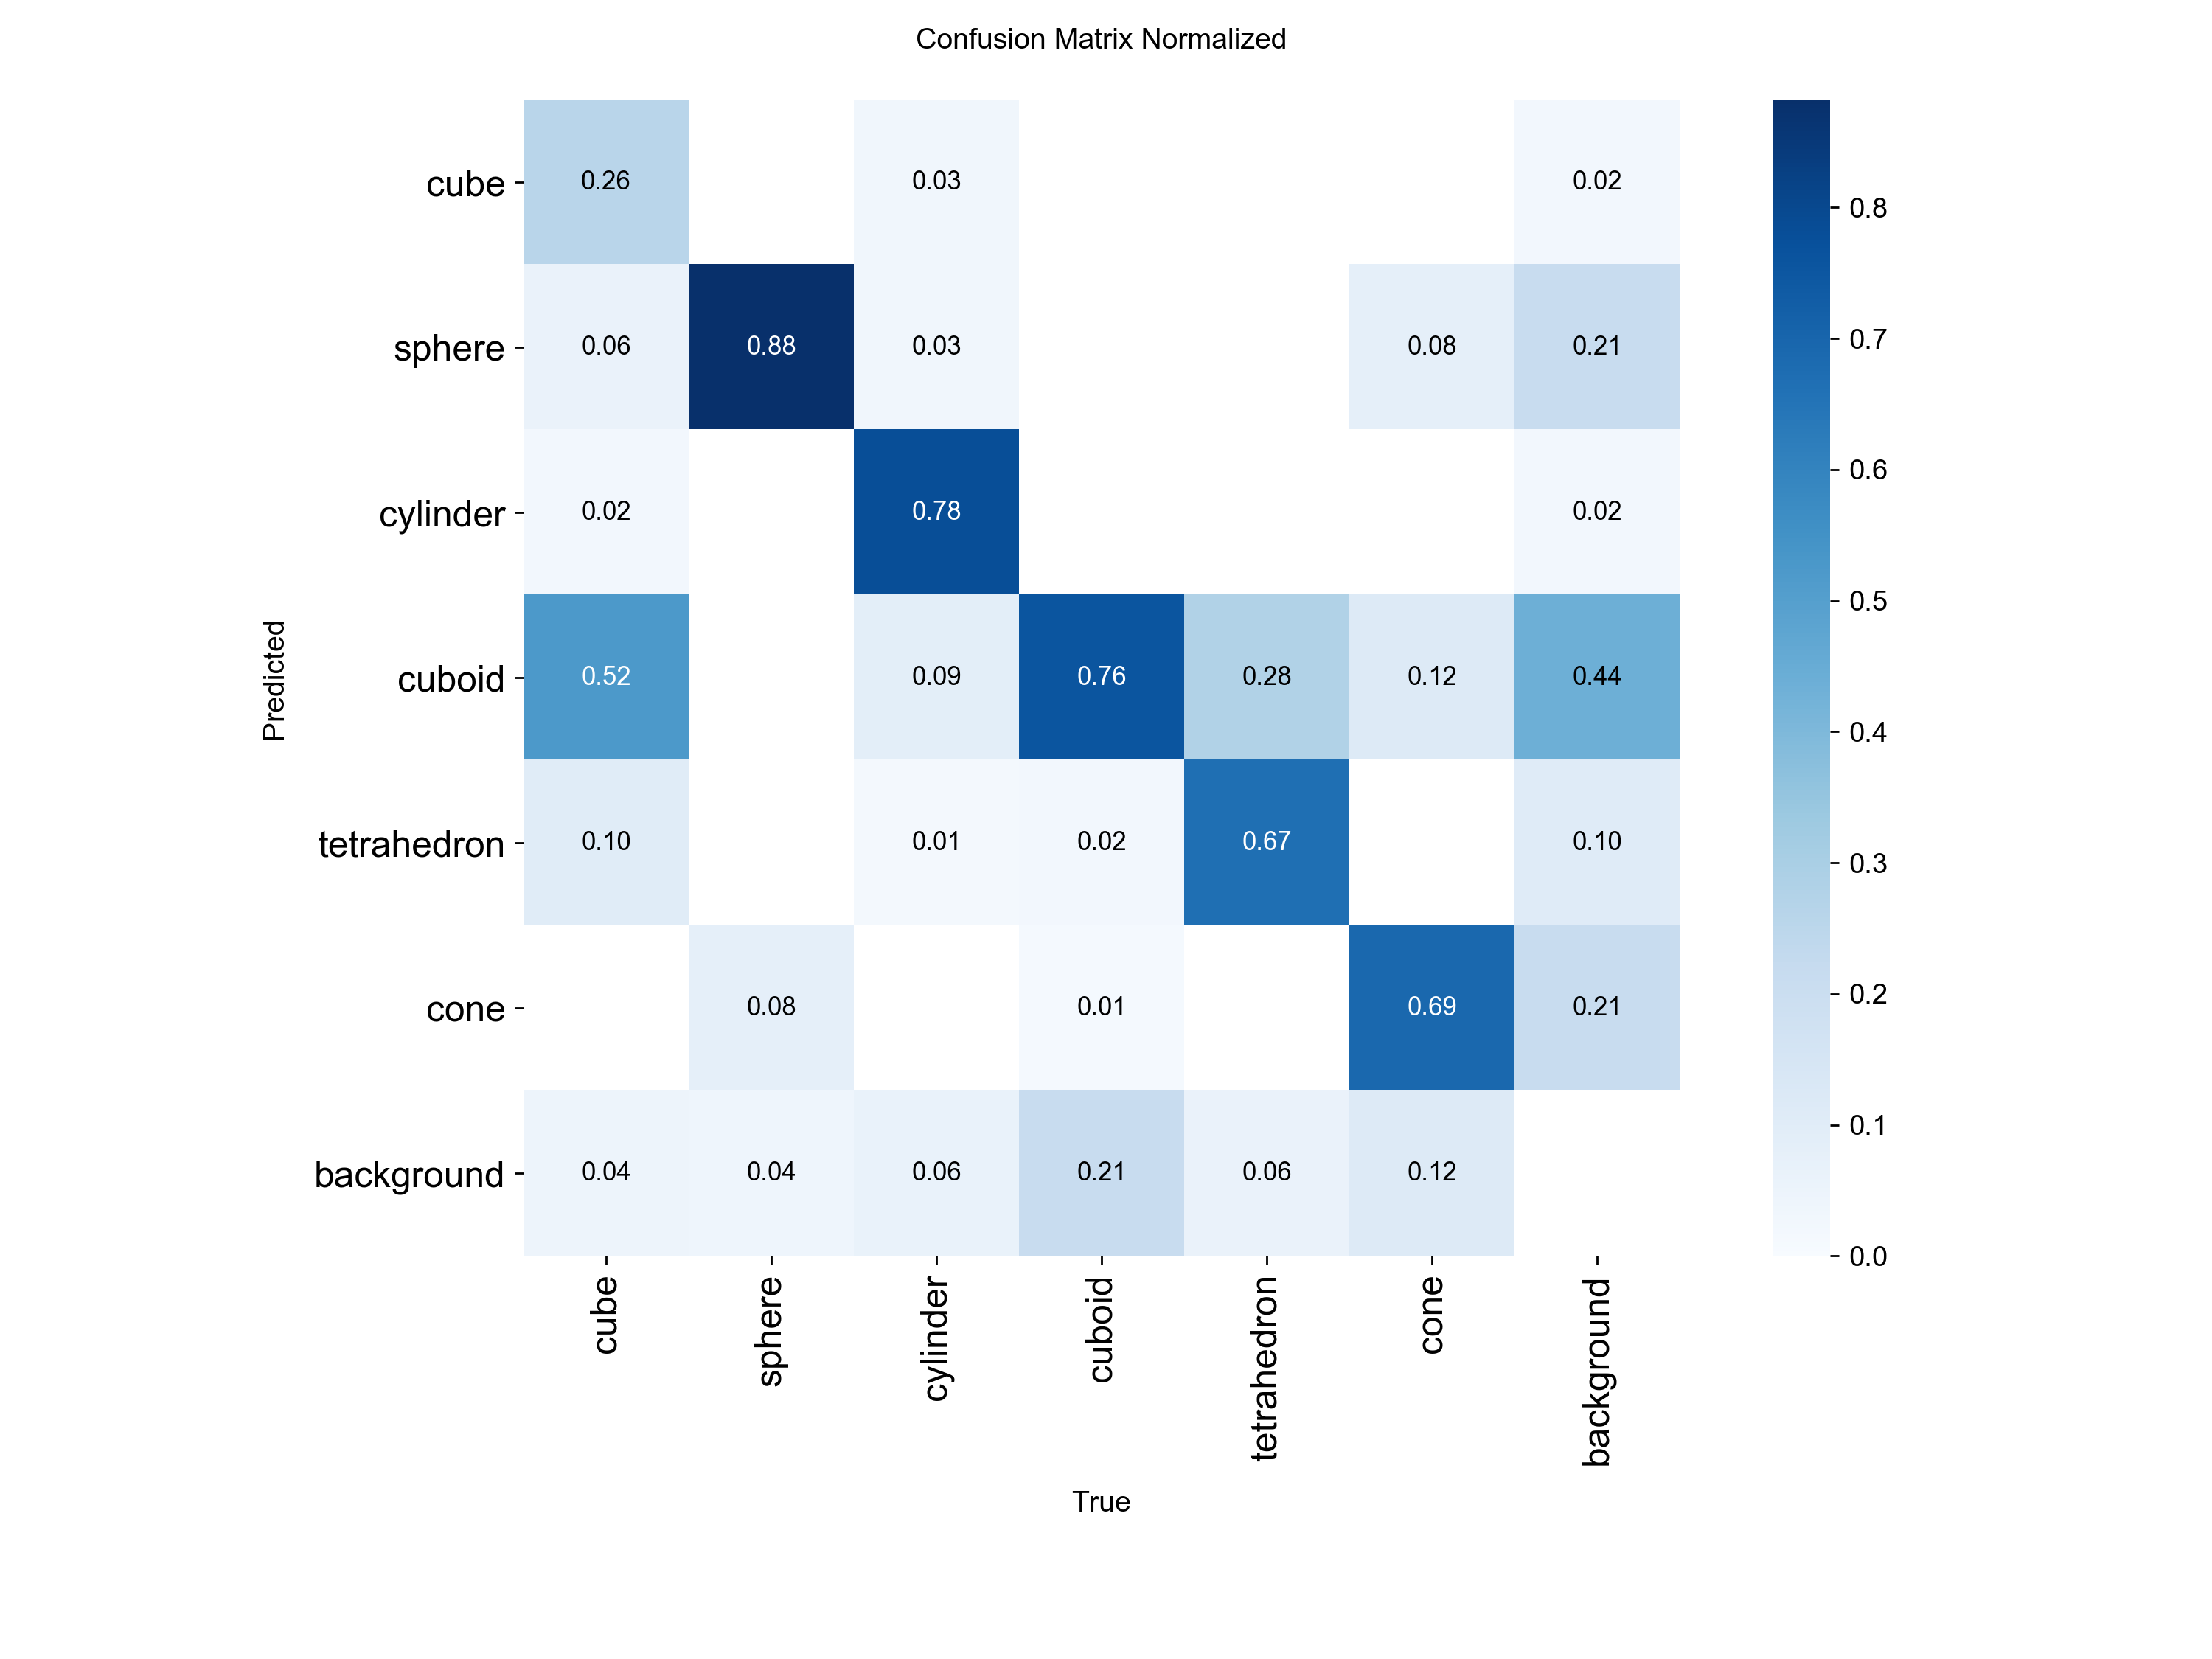
\includegraphics[width=0.9\textwidth]{./graf/conf_matrix/E1.png}
        \caption{Wariant $E_1$: YOLO26n 640 RGB.}
        \label{fig:confusion_matrix_e1}
    \end{subfigure}
    \hfill
    \begin{subfigure}{\textwidth}
        \centering
        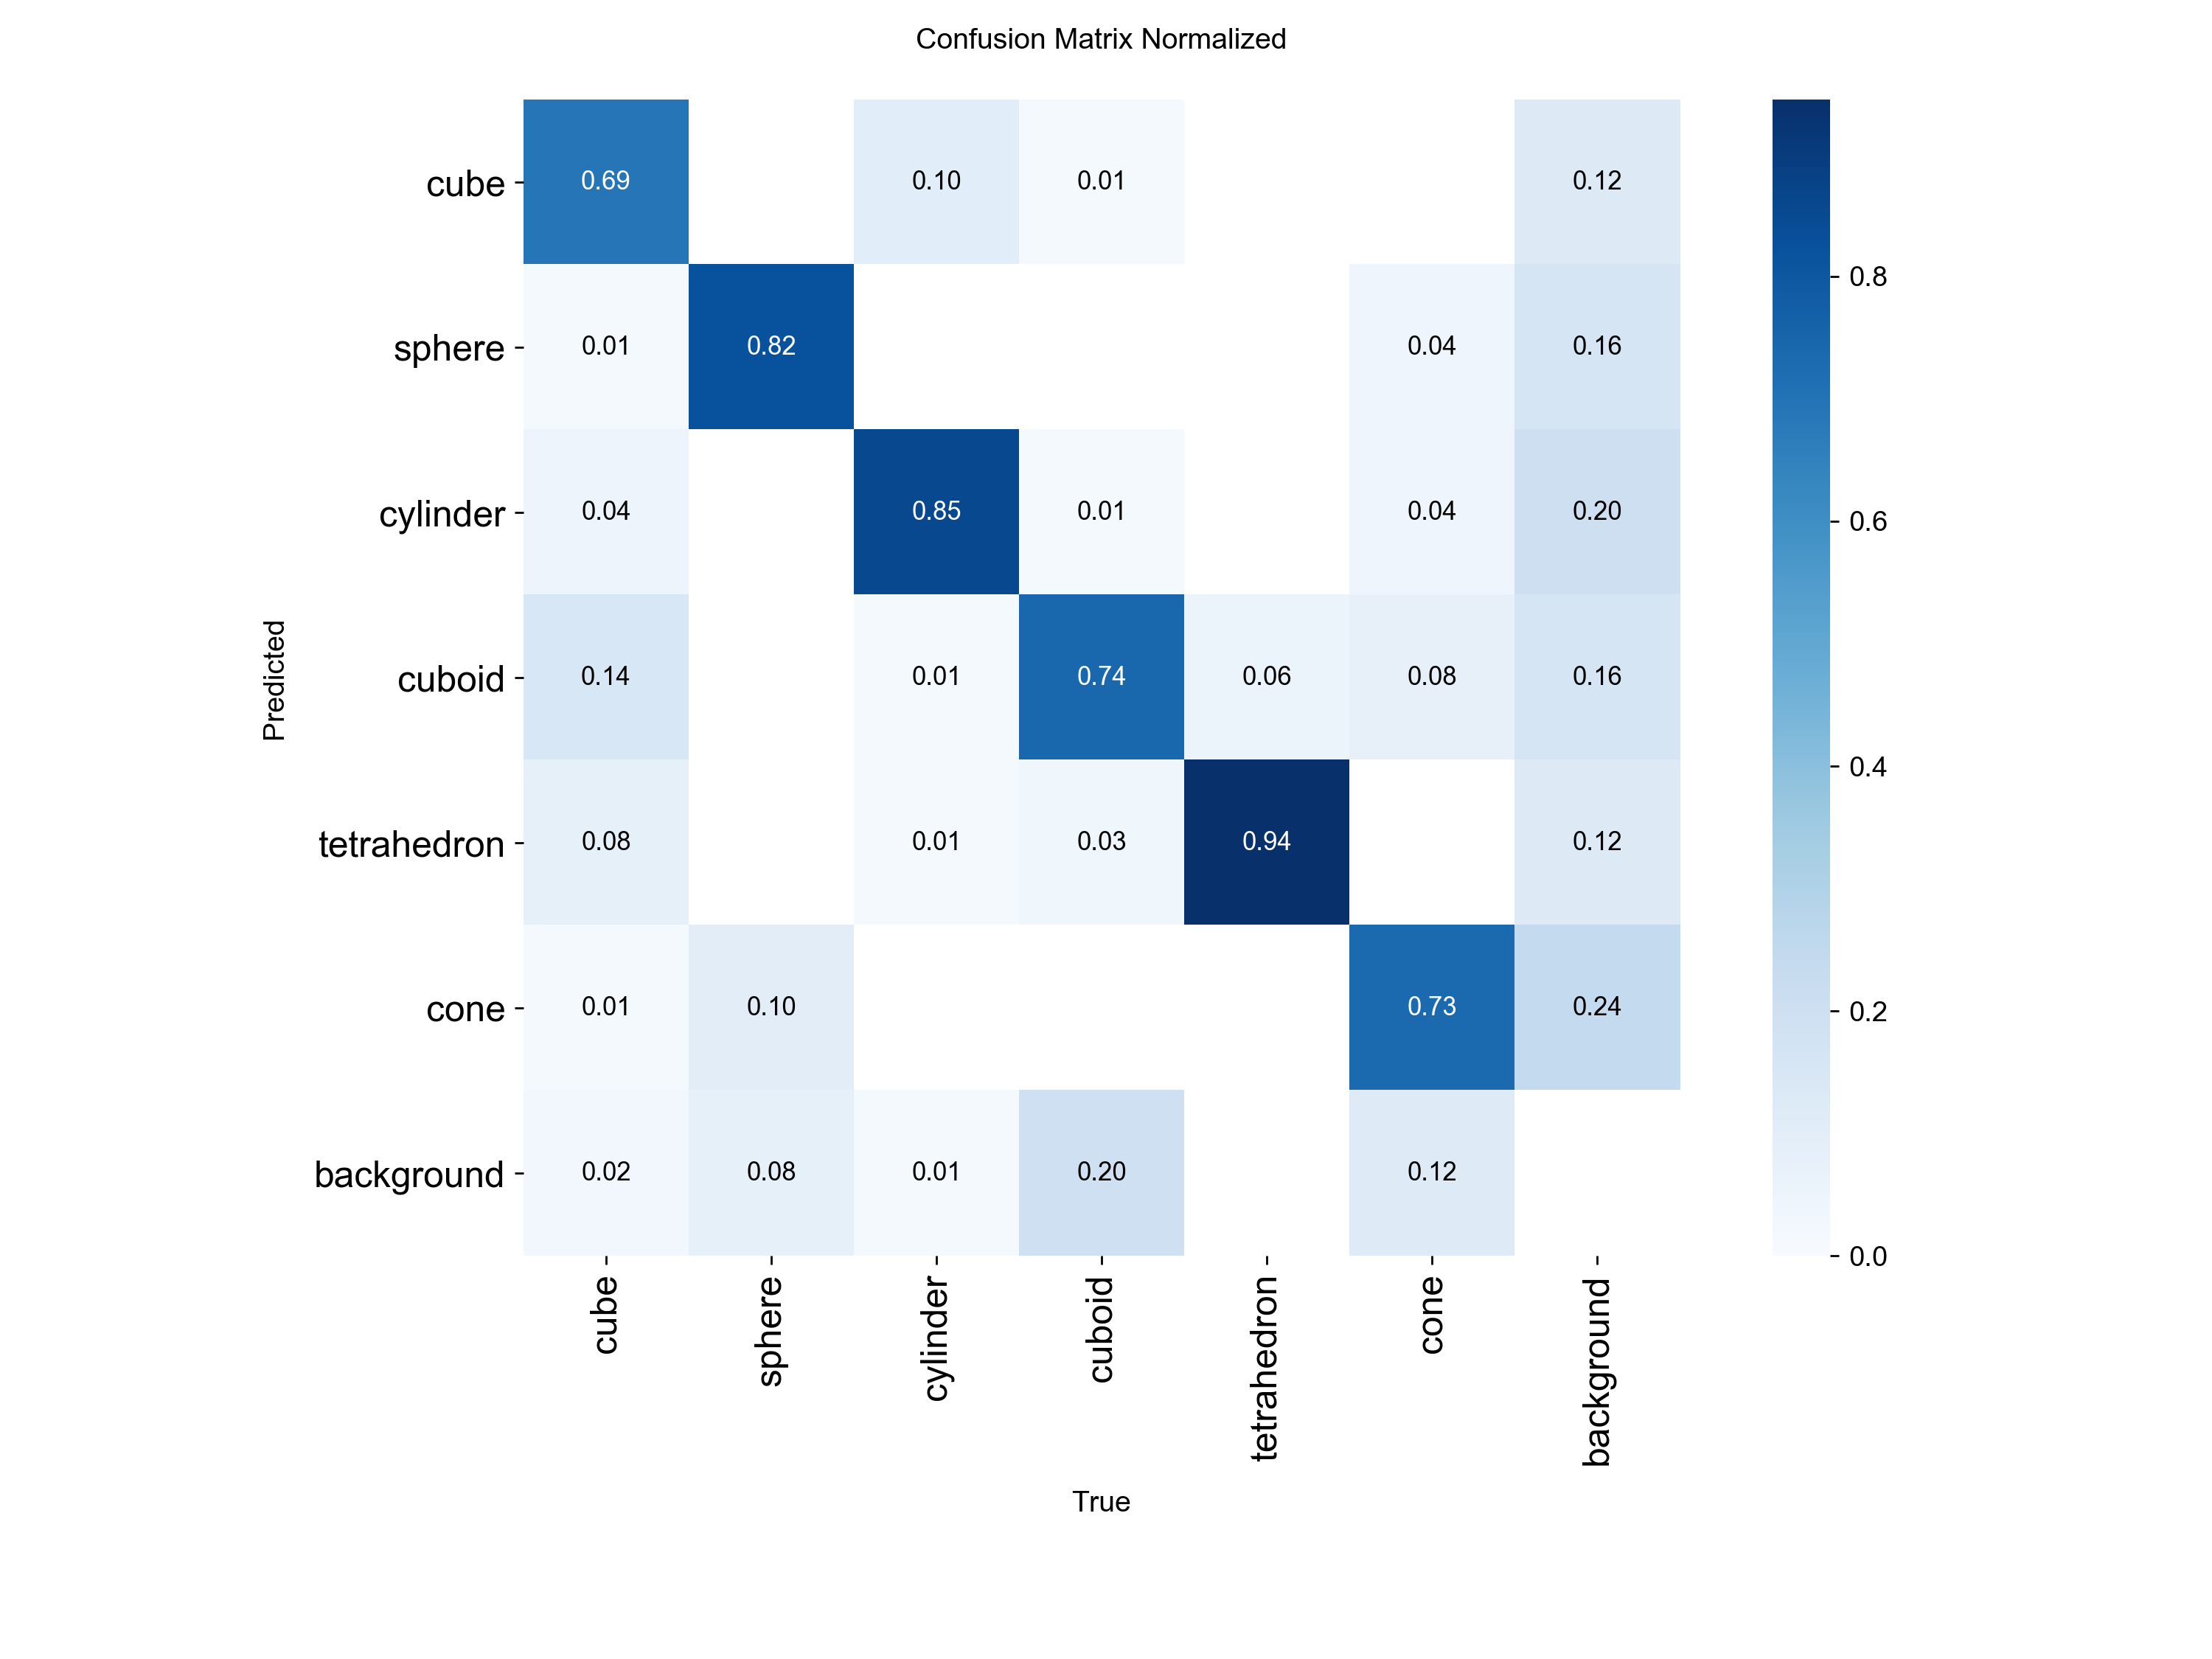
\includegraphics[width=0.9\textwidth]{./graf/conf_matrix/E3.png}
        \caption{Wariant $E_3$: YOLO26n 1024 RGB.}
        \label{fig:confusion_matrix_e3}
    \end{subfigure}
\end{figure}
\begin{figure}[htbp!]
    \ContinuedFloat\centering
    \begin{subfigure}{\textwidth}
        \centering
        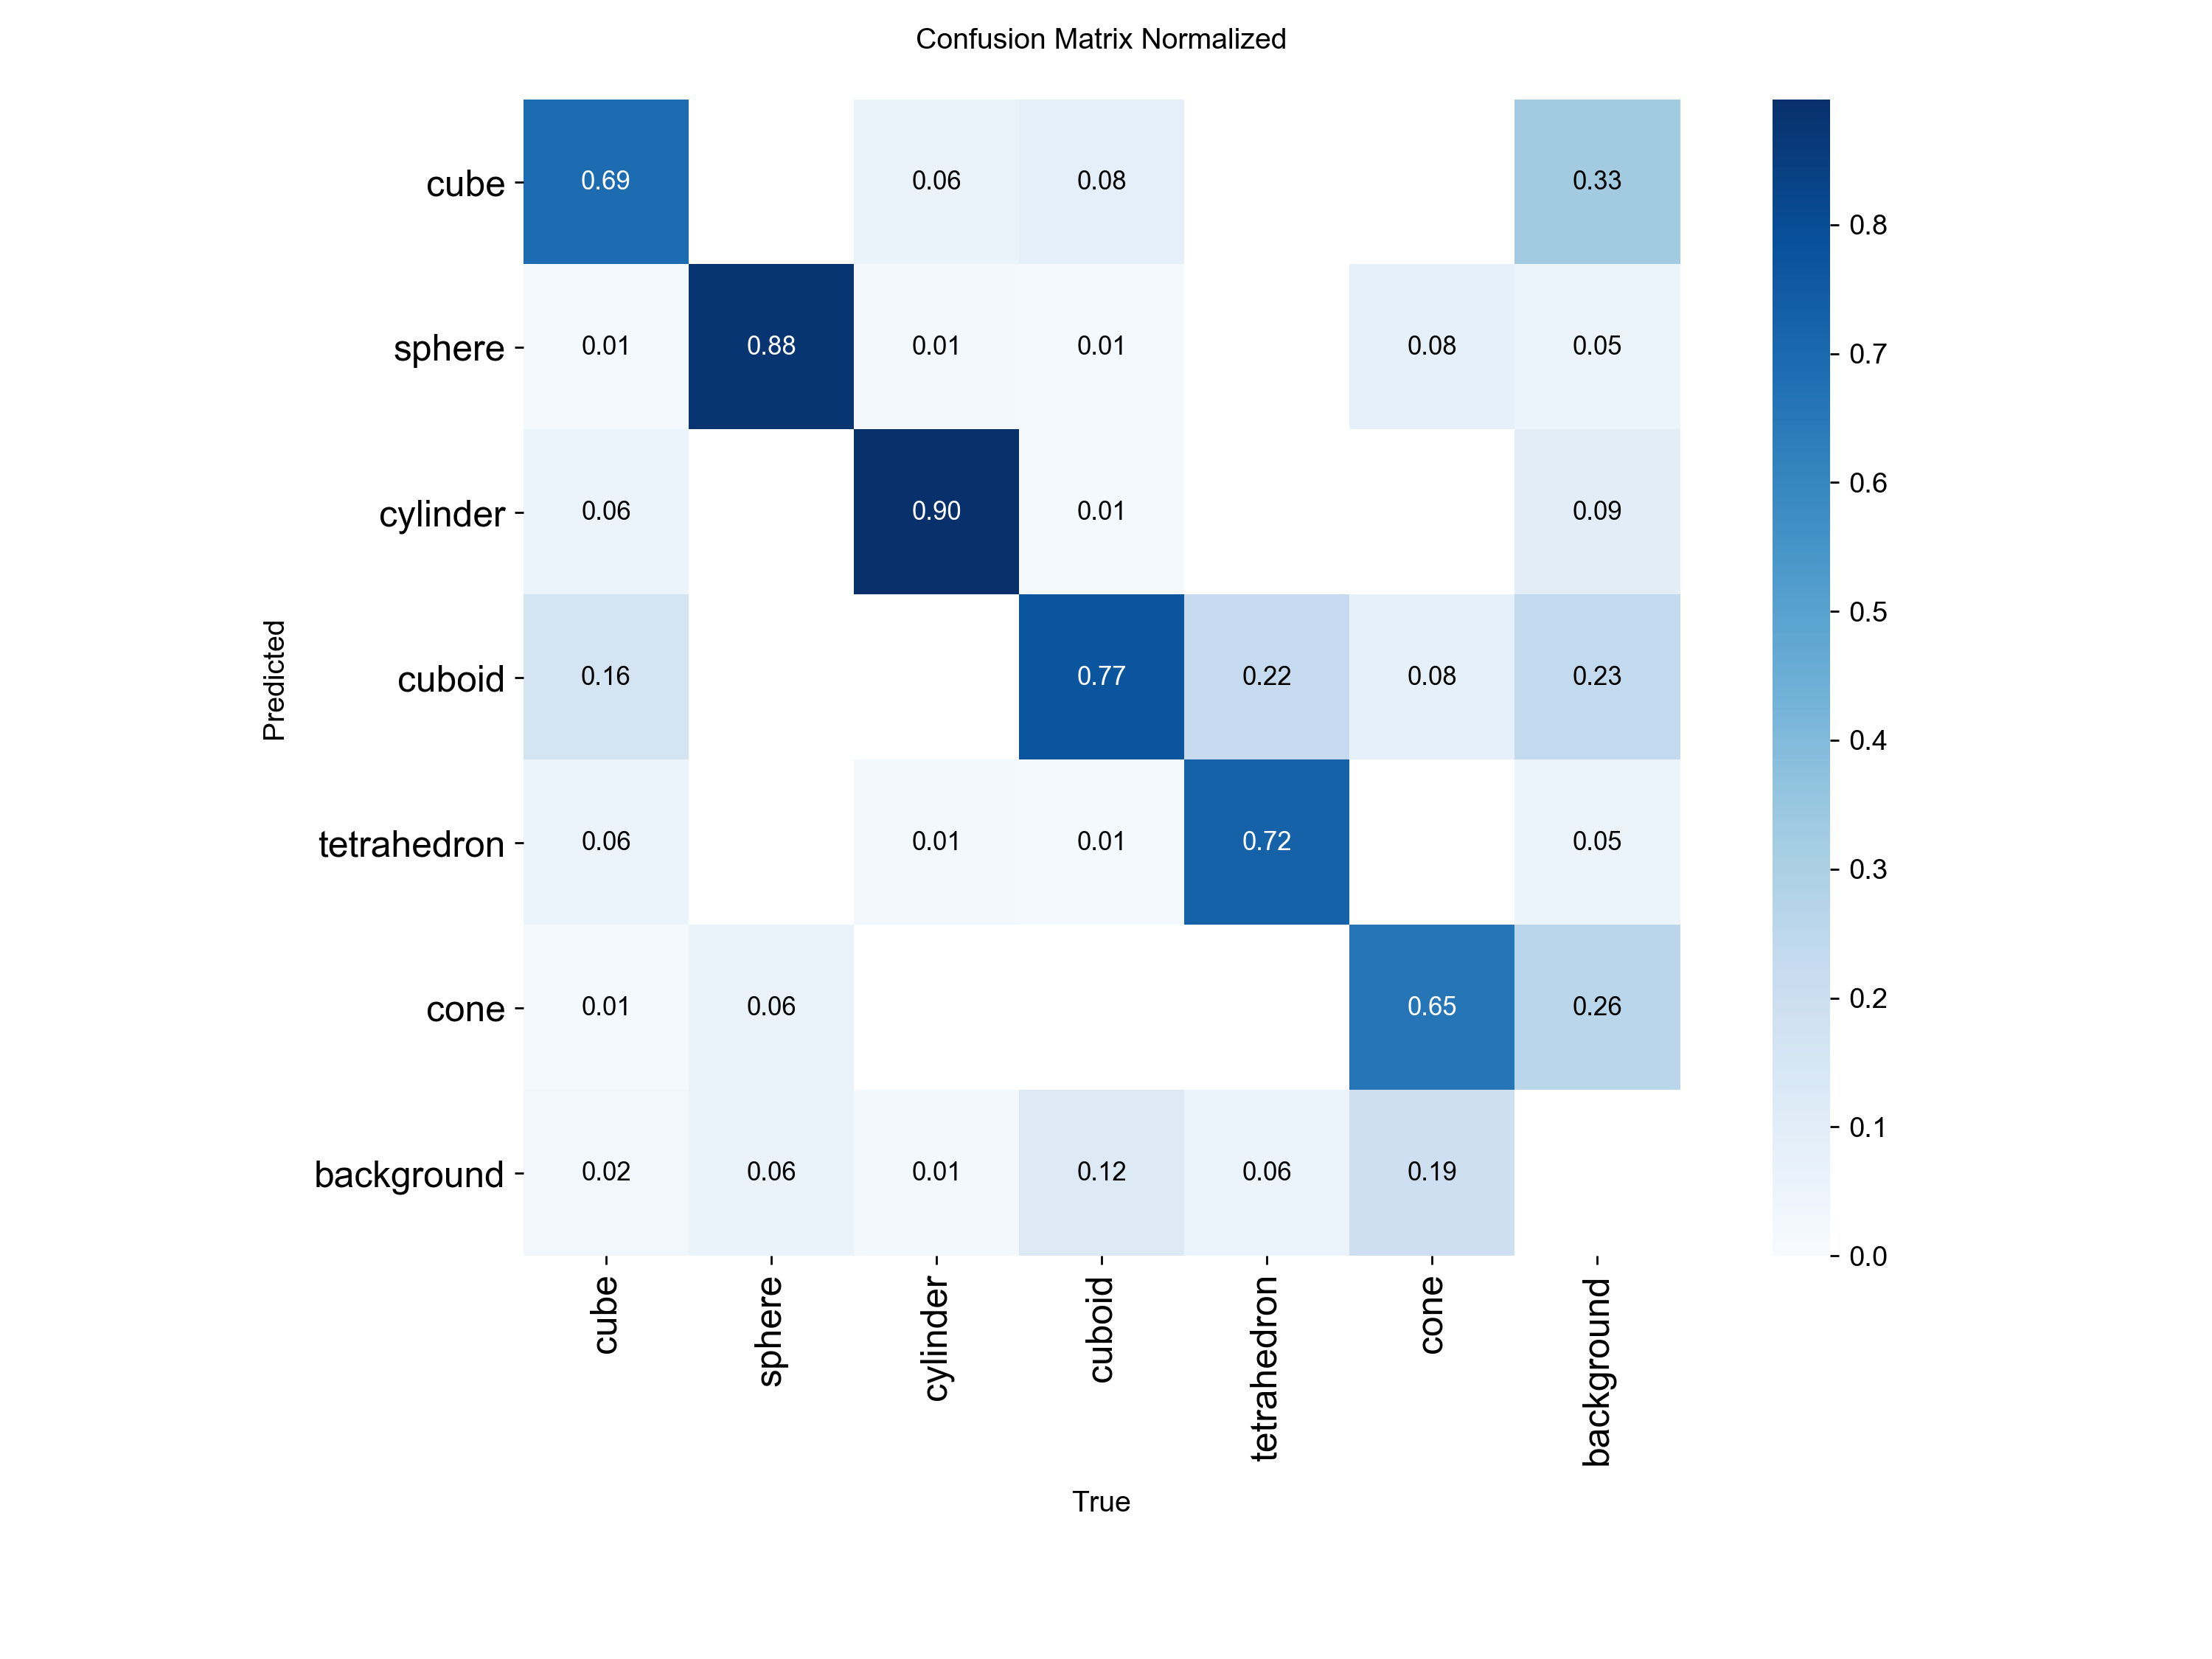
\includegraphics[width=0.9\textwidth]{./graf/conf_matrix/E4.png}
        \caption{Wariant $E_4$: YOLO26s 1024 RGB.}
        \label{fig:confusion_matrix_e4}
    \end{subfigure}
    \hfill
    \begin{subfigure}{\textwidth}
        \centering
        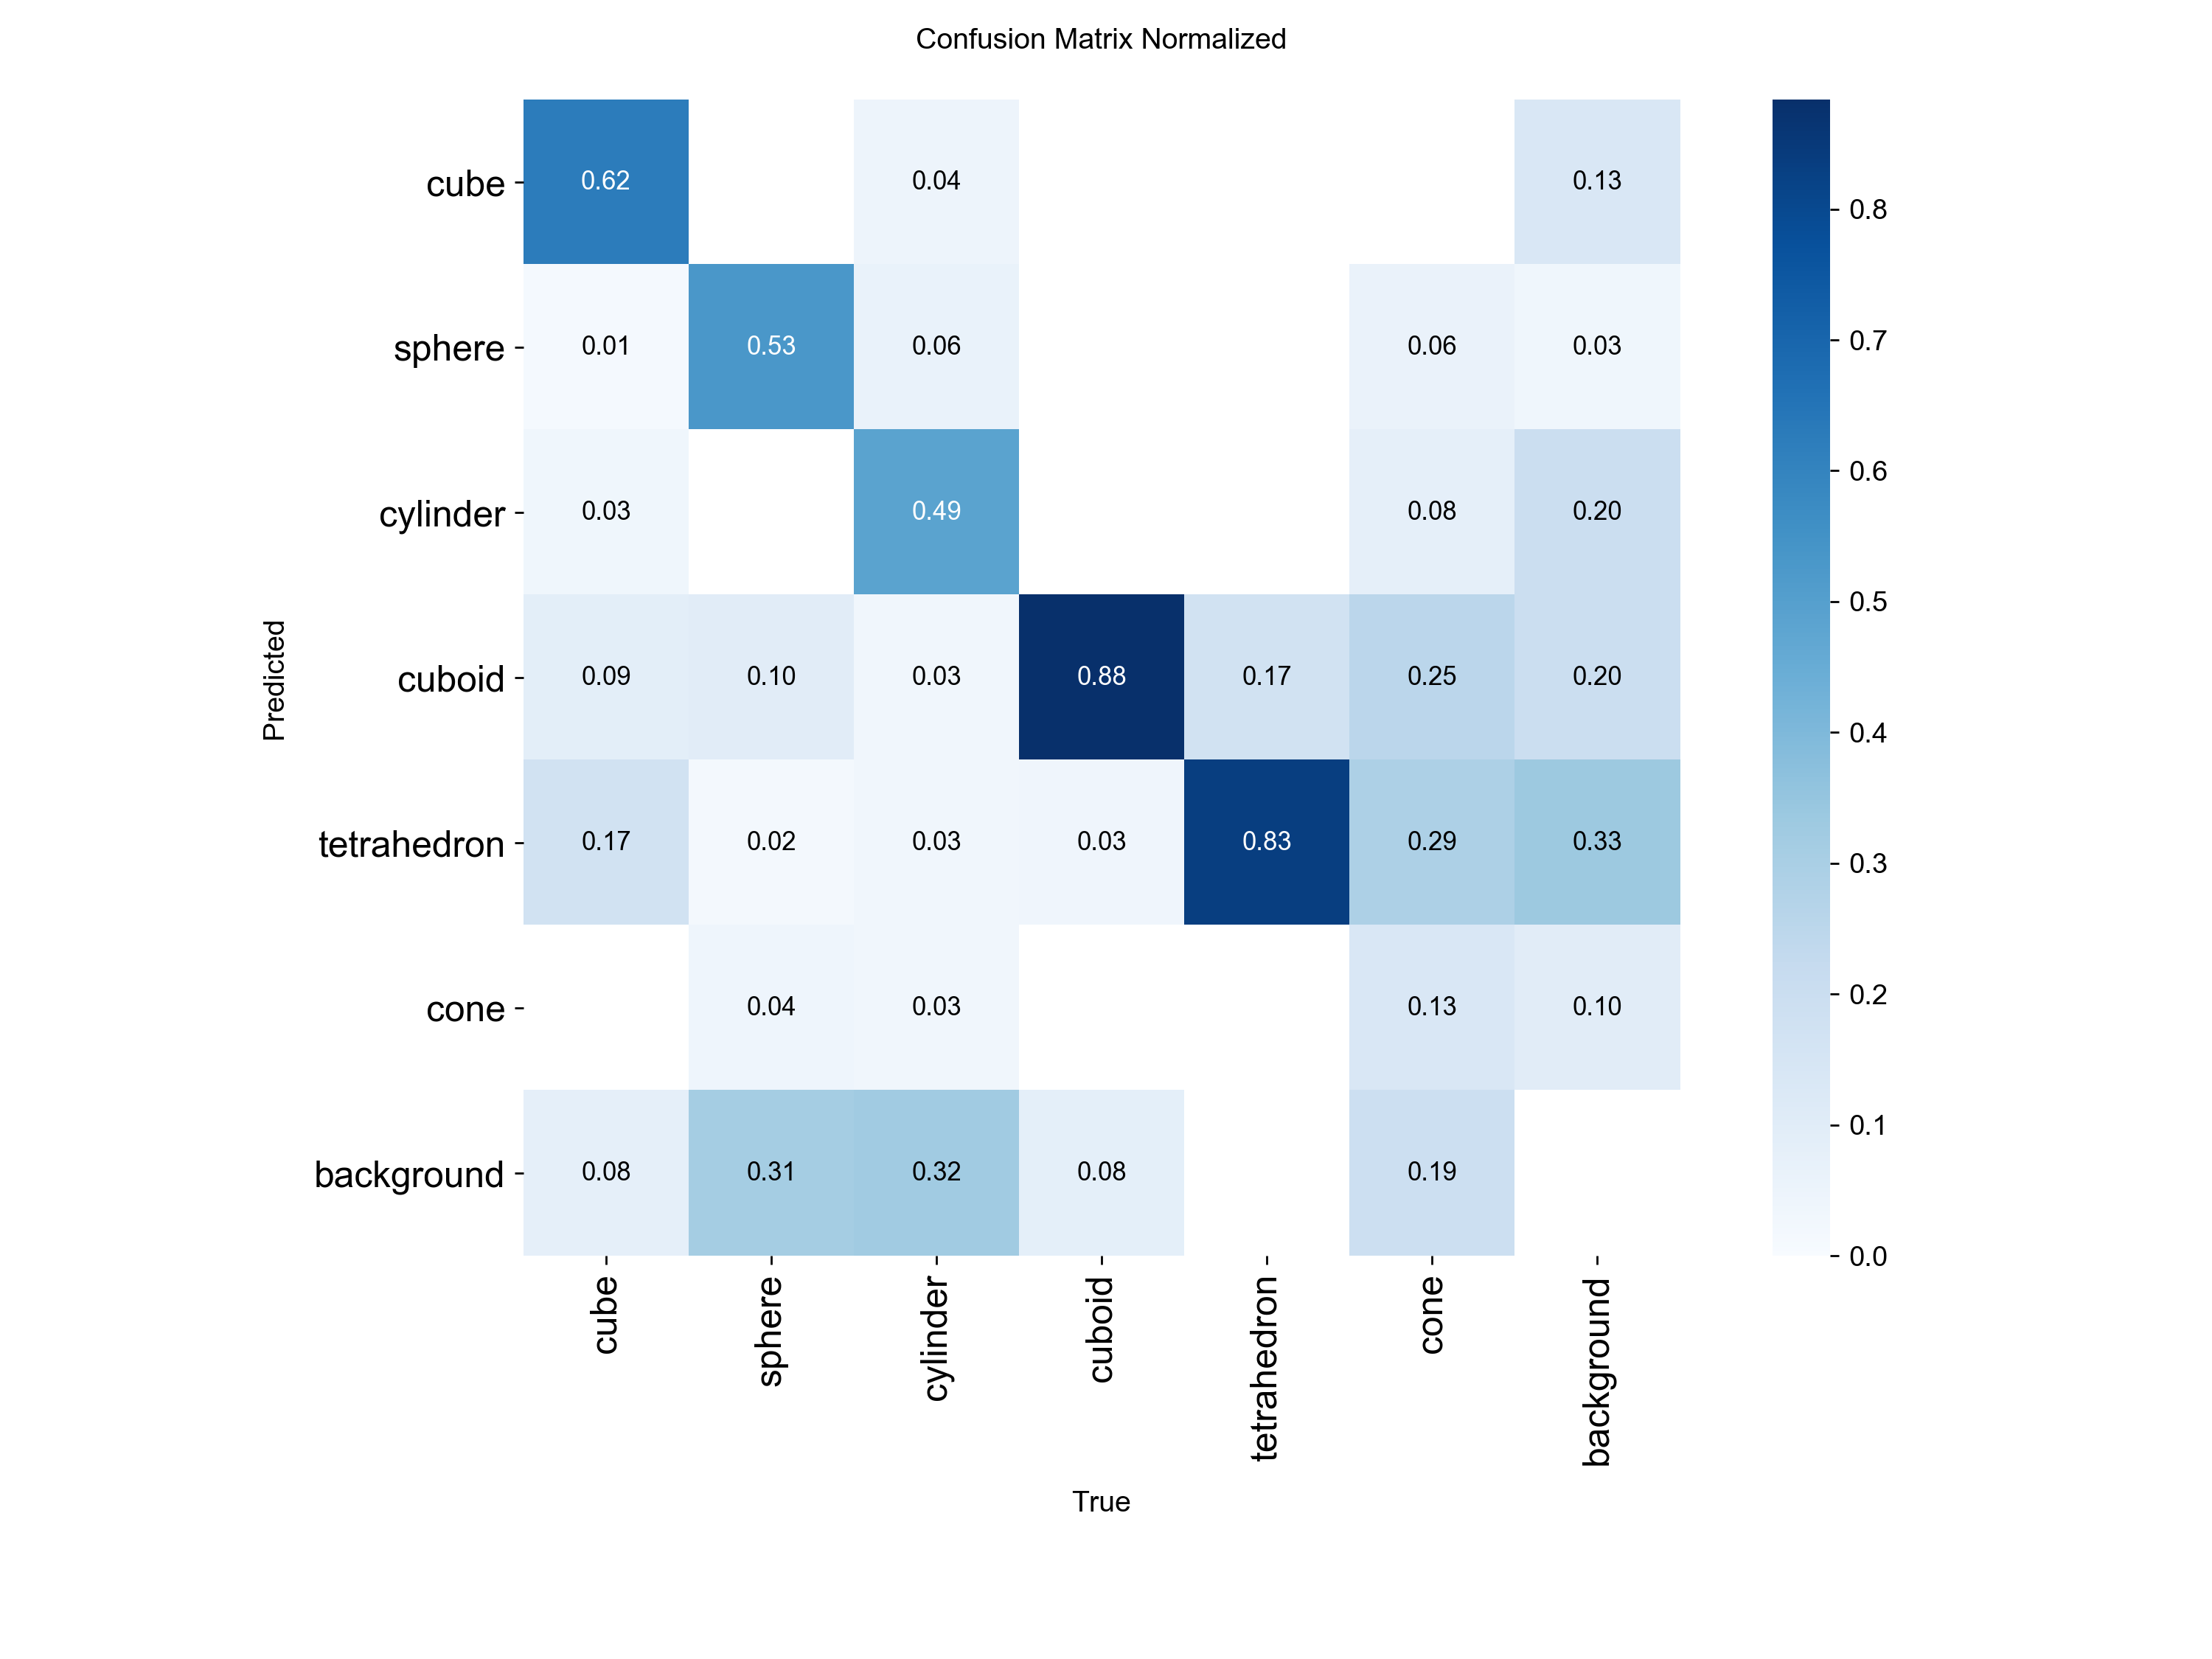
\includegraphics[width=0.9\textwidth]{./graf/conf_matrix/E7.png}
        \caption{Wariant $E_7$: YOLO26n 1024 grayscale.}
        \label{fig:confusion_matrix_e7}
    \end{subfigure}

    \caption{Wybrane znormalizowane macierze pomyłek badanych modeli.}
    \label{fig:confusion_matrices}
\end{figure}

Szczególnie wyraźną różnicę zauważyć można porównując modele $E_1$ i~$E_3$, które różnią się jedynie rozmiarem obrazu wejściowego. Pierwszy z~nich ma problemy z~wykrywaniem sześcianów, które bardzo często klasyfikuje jako prostopadłościany. Poprawnie sklasyfikowano jedynie $26\%$ z~nich, a~ponad połowa została przypisana do klasy prostopadłościanów. Zauważamy też, że model często znajduje prostopadłościany w~miejscach, w~których ich nie ma, co może wskazywać na ich nadmierne przypisywanie obiektów do tej klasy. Zwiększenie rozmiaru obrazu wejściowego w~wariancie $E_3$ znacznie poprawiło skuteczność odróżnienia sześcianów od prostopadłościanów, co może wynikać z~zachowania większej ilości szczegółów obrazu, ułatwiających rozróżnienie proporcji, ścian i~krawędzi obu brył.

Podobne zachowanie obserwujemy dla innych klas. Zwiększenie rozdzielczości skutkuje wzrostem poprawnych klasyfikacji z~$78\%$ do $85\%$ dla walca i~z~$67\%$ do $94\%$ dla czworościanu. Nie wszystkie klasy jednak reagują w~ten sam sposób -- dla kuli ilość poprawnych predykcji spada o~$6$ punktów procentowych, a~dla prostopadłościanu pozostaje na zbliżonym poziomie. Te wyniki uzupełniają wnioski płynące z~eksperymentu~B: zwiększenie rozdzielczości obrazu poprawia globalną zdolność modelu do wykrywania obiektów, ale nie dla każdej klasy osobno.

Przy zestawieniu modeli $E_3$ i~$E_4$ widzimy zgoła inny obraz. Zwiększenie skali modelu poprawia udział poprawnych detekcji dla kuli, walca i~prostopadłościanu, ale osiąga znacząco gorsze wyniki dla czworościanu i~stożka. Dla pierwszego z~nich ilość poprawnych detekcji spada o~$22$ punkty procentowe, a~dla drugiego o~$8$ punktów procentowych. Niewielka przewaga w~$mAP50\text{-}95$ wariantu $E_4$ nie wynika więc z~równomiernej poprawy detekcji wszystkich klas, a~raczej z~ograniczenia części błędów. Jednocześnie, większy model popełnia więcej błędów w~innych przypadkach, co stanowi kolejny argument za wyborem wariantu $E_3$ do zastosowania w~systemie.

Największą zmianę w~charakterze i~ilości błędów detekcji obserwujemy w~przypadku wariantu $E_7$, korzystającego z~obrazów w~odcieniach szarości. Usunięcie informacji o~kolorze nie wpływa równomiernie na zdolność rozpoznawania poszczególnych klas. Na wysokim poziomie pozostaje wykrywanie prostopadłościanów i~czworościanów, osiągając wyniki powyżej $83\%$. W~porównaniu z~modelem $E_3$ zdecydowanie gorzej radzi sobie z~wykrywaniem kuli i~walca -- w~obu przypadkach spadek wyniósł ponad $29$ punktów procentowych. Najgorszy wynik został zanotowany dla klasy stożka, którego poprawne wykrycie odbyło się tylko w~$13\%$ przypadków, a~$29\%$ z~nich zostało sklasyfikowane jako czworościany. Wskazuje to, że usunięcie informacji o~barwie szczególnie wpływa na zdolność modelu do rozróżniania tej klasy od innych.

Model pracujący na obrazach w~odcieniach szarości wykazuje również większą liczbę pominiętych obiektów. Wiersz \english{background} macierzy odpowiada obiektom referencyjnym, do których nie dopasowano żadnej predykcji. Dla modelu $E_7$ udział takich przypadków wynosi $31\%$ dla kuli i~$32\%$ dla walca, podczas gdy model $E_3$ wartości te osiągają odpowiednio $8\%$ i~$1\%$. Dla pozostałych klas wyniki pozostają na zbliżonym poziomie. Pogorszenie wyników wynika więc nie tylko z~błędnego przypisania klas, ale również ze zwiększonej liczby niewykrytych obiektów.

Macierze pomyłek nie są jednak jedynym źródłem informacji o~błędach detekcji. Warto również przyjrzeć się krzywym precyzji i~czułości, które pozwalają ocenić jak zmienia się kompromis pomiędzy tymi dwoma metrykami w~zależności od progu decyzyjnego. Z~tego względu analizę uzupełniono o~wykresy krzywych precision--recall. Na rysunku~\ref{fig:pr_curves} zestawiono je dla wariantów $E_3$ oraz $E_7$. Reprezentują one wybraną konfigurację docelową oraz wpływ ograniczenia koloru na jakość detekcji.

\begin{figure}[htbp!]
    \centering
    \begin{subfigure}{\textwidth}
        \centering
        
\includegraphics[width=\textwidth]{./graf/pr_curve/E3.png}
        \caption{Wariant $E_3$: YOLO26n 1024 RGB.}
        \label{fig:pr_curve_e3}
    \end{subfigure}
    \begin{subfigure}{\textwidth}
        \centering
        
\includegraphics[width=\textwidth]{./graf/pr_curve/E7.png}
        \caption{Wariant $E_7$: YOLO26n 1024 grayscale.}
        \label{fig:pr_curve_e7}
    \end{subfigure}

    \caption{Krzywe precision--recall modeli $E_3$ i~$E_7$ uzyskane na zbiorze testowym.}
    \label{fig:pr_curves}
\end{figure}

Krzywe PR umożliwiają ocenę, w~jaki sposób wzrost czułości oddziałuje na precyzję detekcji poszczególnych klas. Ich przebieg ukazuje rozwinięcie informacji przekazywanych przez metryki AP i~$mAP$, ponieważ pozwala ocenić zachowanie modelu w~całym zakresie kompromisu pomiędzy tymi dwoma metrykami. Porównanie wariantów $E_3$ i~$E_7$ pozwala sprawdzić, czy pogorszenie jakości spowodowane usunięciem informacji o~kolorze dotyczy pojedynczego progu działania, czy też jest widoczne w~szerszym zakresie pracy modelu.

Dla modelu $E_3$ średnia wartość AP przy progu IoU równym $0,5$ wyniosła $0,862$. Najwyższe wartości uzyskano dla klas kuli i~walca, które osiągnęły wartości powyżej $0,94$, a~także dla sześcianu, którego AP50 wyniosło $0,875$. Najsłabszym wynikiem spośród wszystkich klas charakteryzuje się prostopadłościan, dla którego wartość wyniosła $0,732$. Mimo obserwowanej na macierzach pomyłek tendencji do mylenia sześcianów z~prostopadłościanami, model prezentuje wysoką precyzję dla większości klas, również po zwiększeniu progu czułości.

Znacznie bardziej zróżnicowany przebieg krzywych PR obserwujemy w~przypadku wariantu $E_7$. W~jego przypadku $mAP50$ spada do wartości $0,621$. Model osiąga najwyższe wyniki dla prostopadłościanu i~sześcianu, dla których wartości AP50 są powyżej $0,84$, pozostając zbliżonymi do modelu pracującego w~przestrzeni kolorowej. Pozostałe klasy osiągają jednak znacznie niższe wyniki. Najniższe wartości uzyskano dla stożka i~czworościanu, dla których AP50 wyniosło około $0,41$. Ma to swoje odzwierciedlenie w~macierzy pomyłek, w~której widać, że model ma największe problemy z~wykrywaniem stożków.

Porównanie krzywych pochodzących z~tych dwóch modeli potwierdza więc, że pogorszenie wyników po usunięciu informacji o~kolorze nie jest ograniczone do jednego progu czułości, a~dotyczy całego zakresu pracy modelu. Różnice utrzymują się w~szerokim zakresie kompromisu, a~ich wielkość jest silnie zależna od klasy obiektu. Szczególnie istotny jest fakt, że oba modele zachowują wysokie wartości AP50 dla sześcianu i~prostopadłościanu niezależnie od wykorzystania koloru do detekcji. Niestety, dla pozostałych klas wartość ta ulega znacznemu pogorszeniu. Wskazuje to, że model wykorzystuje informacje o~kolorze w~procesie detekcji, lecz jego znaczenie nie jest jednakowe dla wszystkich klas.

Poza zależnościami precision-recall z~punktu widzenia systemu istotny jest również wybór progu pewności predykcji. Jego zbyt niskie ustawienie może zwiększyć liczbę wykrywanych obiektów, jednak może również prowadzić do zwiększenia ilości fałszywych predykcji. Z~drugiej strony, zbyt rygorystyczne ustawienie progu ograniczy udział błędnych wskazań kosztem pominięcia części obiektów. Wybór optymalnej wartości progu, w~którym zachowany jest najlepszy kompromis pomiędzy precyzją a~czułością, może zostać dokonany na podstawie krzywej $F1$. Zależność $F1$-score od progu pewności predykcji dla wariantu $E_3$ przedstawiono na rysunku~\ref{fig:f1_curve_e3}.

\begin{figure}[ht]
    \centering
    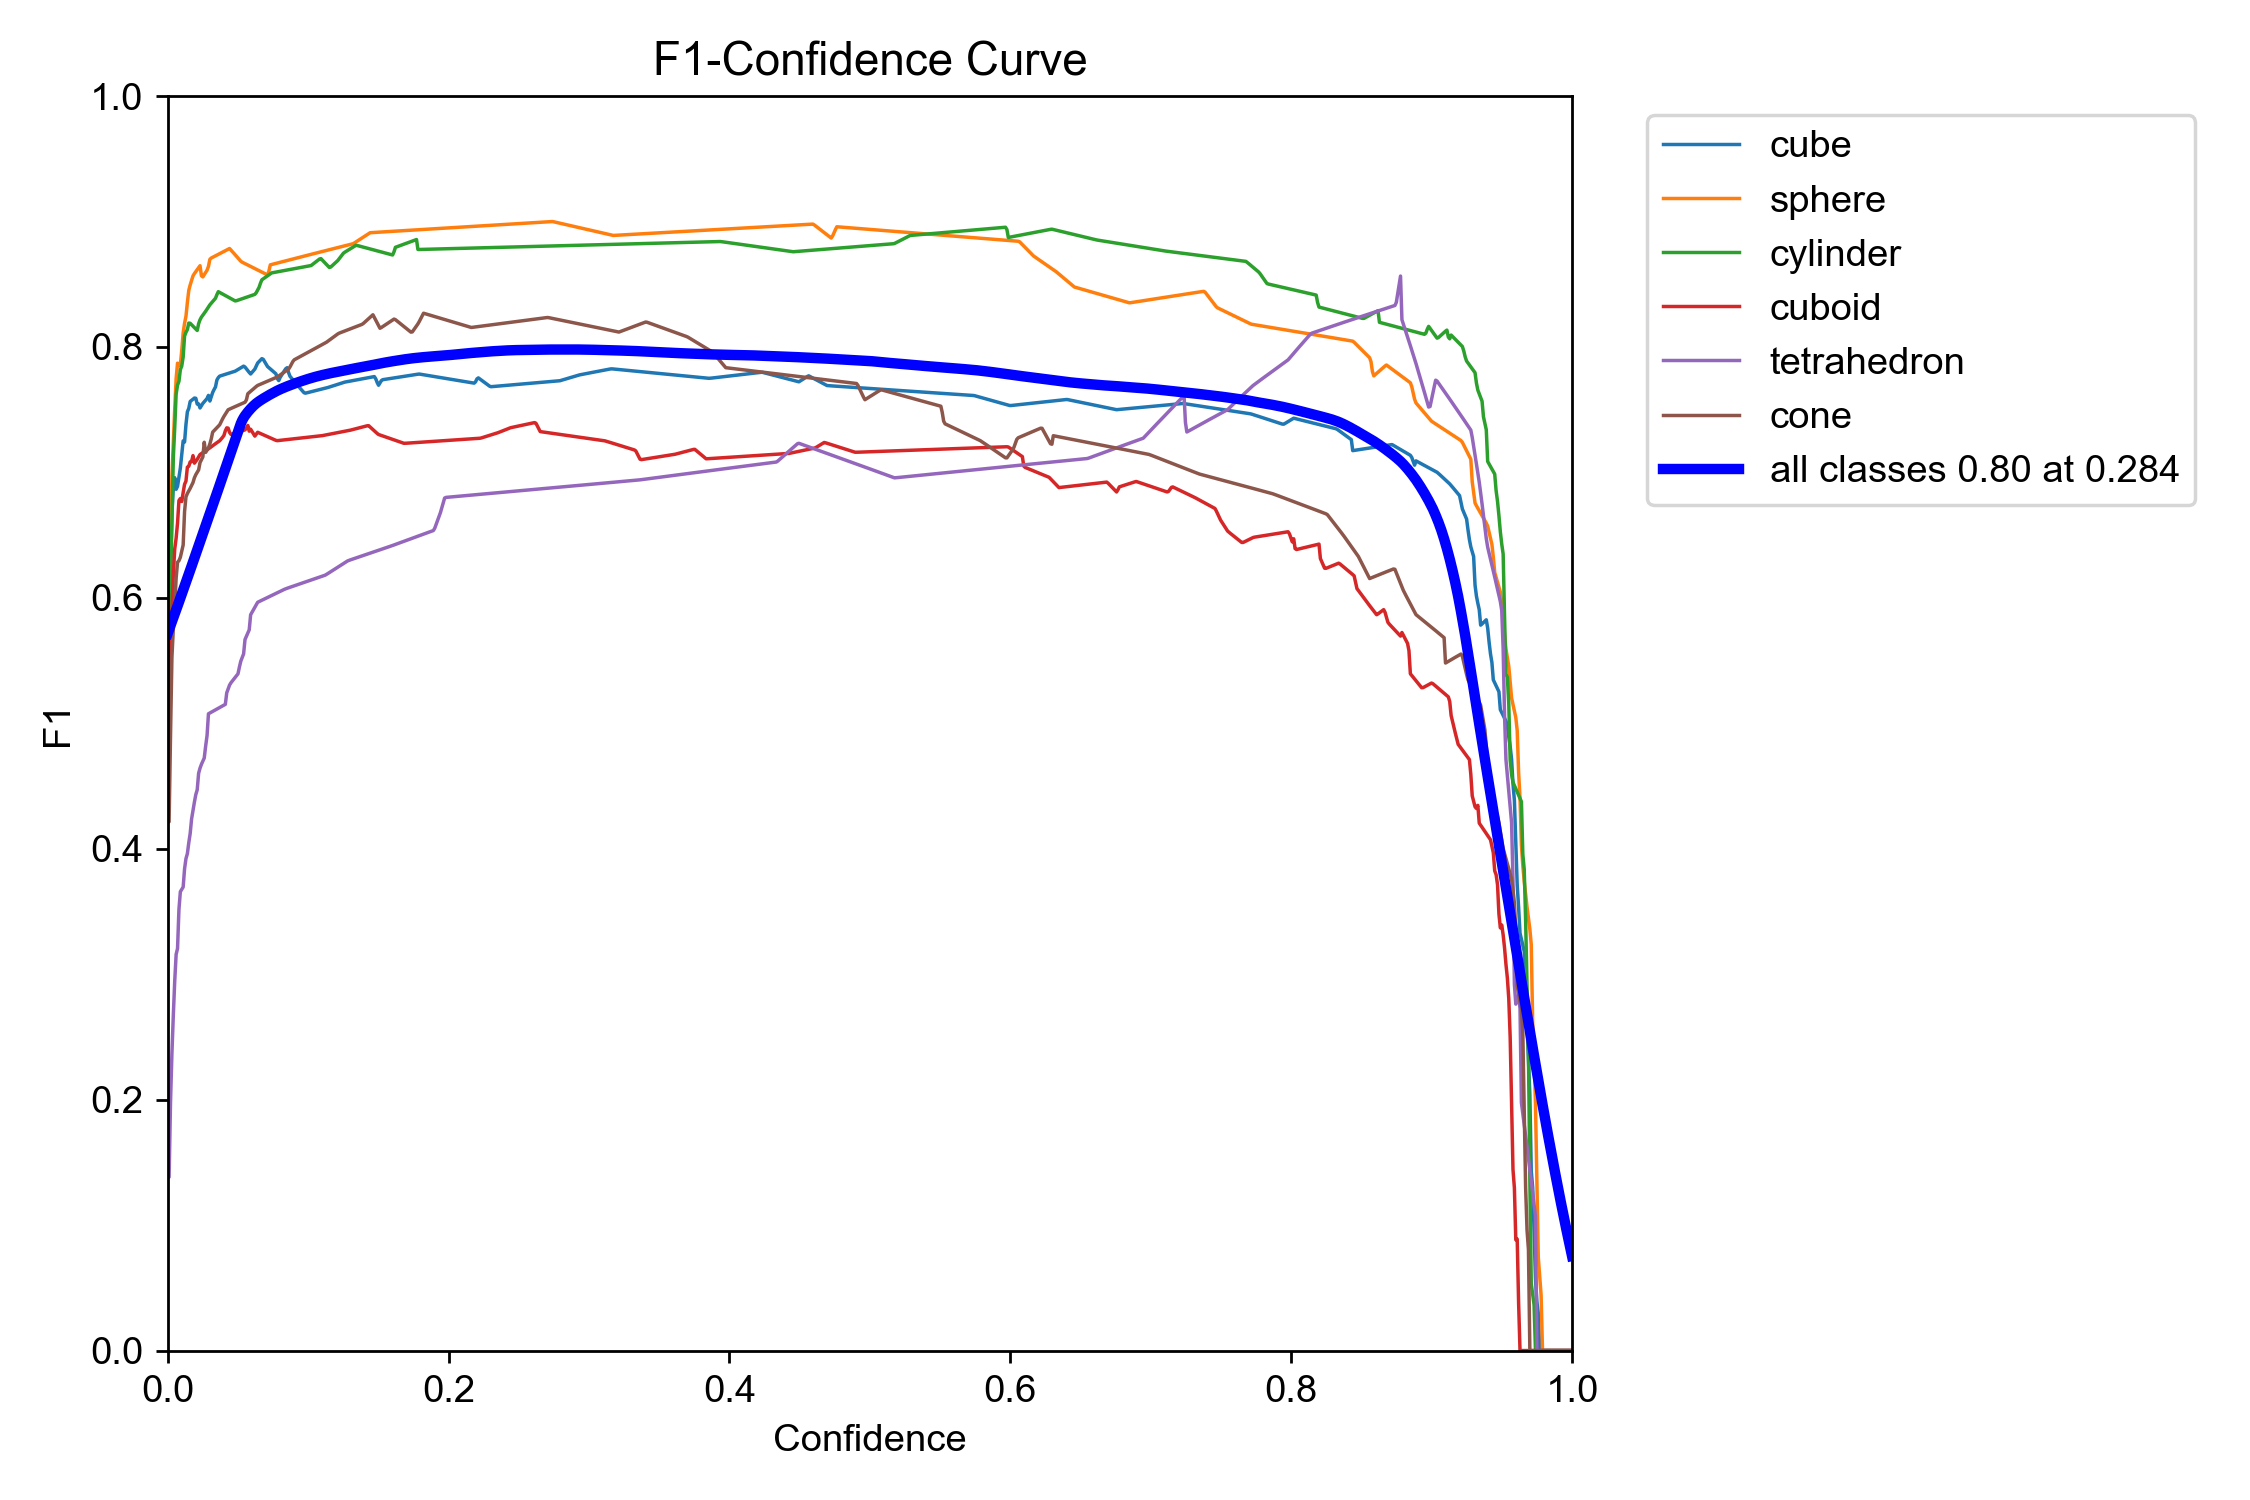
\includegraphics[width=0.9\textwidth]{./graf/E3_F1_curve.png}
    \caption{Krzywa $F1$ dla wariantu $E_3$.}
    \label{fig:f1_curve_e3}
\end{figure}

Dobór odpowiedniej wartości progu jest szczególnie ważny w~kontekście docelowego systemu, ponieważ wpływa on bezpośrednio na to, które detekcje zostaną uznane za wystarczająco pewne i~przekazane do dalszego przetwarzania. Wynik benchmarku jakościowego może więc posłużyć nie tylko do porównania modeli, ale przede wszystkim do doboru parametrów pracy wybranego modelu $E_3$ w~systemie docelowym.

Dla modelu YOLO26n 1024 RGB, który został wskazany jako wariant docelowy, najwyższa wartość krzywej $F1$ jest osiągana przy progu pewności predykcji równym około $0,284$ i~wynosi około $0,8$. W~tym obszarze zachowany jest najlepszy kompromis precyzji i~czułości. Przy zwiększaniu progu możemy zauważyć stopniowy spadek wartości wskaźnika, a~wysokie wartości pewności -- powyżej $0,9$ -- prowadzą do załamania się krzywej i~nagłego spadku wartości $F1$-score. Wartość progu około $0,284$ może więc zostać przyjęta jako punkt odniesienia przy konfiguracji systemu docelowego, ale nie należy jej traktować jako wartości ostatecznej. Koszty poniesione przez błędne detekcje i~pominięte obiekty nie muszą być jednakowe w~każdym przypadku, dlatego ostateczny próg powinien zostać dobrany zależnie od oczekiwanego działania systemu. W~szczególności zasadne może być jego zwiększenie celem ograniczenia błędnych informacji przekazywanych użytkownikowi końcowemu, kosztem częstszego pomijania obiektów.

Analiza macierzy pomyłek i~krzywych pokazuje, że różnice poszczególnych modeli nie sprowadzają się wyłącznie do zmian parametrów i~wartości metryk globalnych. Poszczególne zmiany wpływają na charakter i~częstość popełnianych błędów. Zwiększenie rozdzielczości obrazu wejściowego w~największym stopniu ułatwiło modelowi odróżnienie sześcianów od prostopadłościanów, a~zwiększenie skali modelu poprawiło wyniki tylko części klas. Największy wpływ miało usunięcie informacji o~kolorze, ale ono również nie wpłynęło równomiernie na wszystkie klasy. Zdolność rozpoznawania sześcianu i~prostopadłościanu pozostała na wysokim poziomie.

Podczas interpretacji wyników należy jednak pamiętać, że w~zbiorze testowym nie występowała równa liczba klas obiektów. W~przypadku klas reprezentowanych przez małą liczbę obiektów, pojedynczy błąd może mieć znaczący wpływ na wartości widoczne w~znormalizowanej macierzy. Takie zachowanie można zaobserwować w~przypadku klasy czworościanu, która występowała w~zbiorze testowym jedynie $18$ razy. Z~tego względu nie należy wyciągać zbyt daleko idących wniosków na podstawie różnic obserwowanych w~przypadku tej klasy ani formułować wniosków o~statystycznie istotnych różnicach w~skuteczności~\nobreakdash{detekcji}.

Macierze pomyłek i~krzywe PR nie stanowią również pełnego przeglądu wszystkich aspektów detekcji. Model może poprawnie wskazywać klasę obiektu, ale nieprawidłowo określać jego położenie. Taki błąd będzie widoczny w~metryce $mAP50\text{-}95$, ale nie musi być odzwierciedlony w~analizie klas. Z~tego powodu wyniki przedstawione w~tej sekcji należy rozpatrywać łącznie z~wynikami metryk globalnych oraz z~porównaniem wydajności modeli. Dopiero w~ten sposób możliwe jest uzyskanie pełnego obrazu skuteczności detekcji i~charakteru popełnianych błędów.

\section{Dyskusja wyników i~ograniczeń badań}

Przeprowadzone badania pozwoliły ocenić wpływ kilku czynników na jakość detekcji dotykanych obiektów trójwymiarowych. Analiza wykazuje, że w~badanym problemie nie wystarczy jedynie zwiększyć złożoności modelu, aby poprawić jego skuteczność. Znaczący wpływ na wyniki ma również rozdzielczość obrazu wejściowego oraz informacja o~kolorze. Szczególnie uwidacznia się to przy porównaniu rozmiaru modelu i~rozdzielczości wejścia. Zwiększenie skali z~YOLO26n do YOLO26s nie przynosiło jednoznacznej poprawy wszystkich metryk, a~w~niektórych przypadkach pogarszało wyniki. Zwiększenie rozdzielczości z~640 do 1024 pikseli przynosiło natomiast znaczącą poprawę wszystkich analizowanych wartości niezależnie od wybranego wariantu modelu. Może to wskazywać, że w~badanym problemie bardzo ważna jest możliwość uchwycenia szczegółów obrazu, które pozwalają modelowi odróżnić poszczególne klasy obiektów.

Wielkość adnotowanych obiektów w~zbiorze danych może częściowo wyjaśniać poprawę wyników obserwowaną po zwiększeniu rozdzielczości obrazu wejściowego. W~przygotowanym zbiorze danych obiekty zajmowały średnio około $1,51\%$ powierzchni obrazu, a~największy z~nich zajął około $7,31\%$ powierzchni. Różnice w~wielkościach wynikają przede wszystkim z~różnej odległości obiektów od kamery, a~także z~ich zasłonięć palcami. W~takich warunkach zwiększenie rozdzielczości obrazu wejściowego pozwala zachować znacznie więcej szczegółów, które mogą być istotne w~procesie detekcji. Wniosek ten dotyczy jednak wyłącznie modeli uczonych na przygotowanym zbiorze danych i~nie może być uogólniany na inne zadania detekcji obiektów.

Bardzo istotnym wynikiem jest duży spadek skuteczności detekcji po usunięciu informacji o~barwie. W~każdym z~badanych przypadków zaobserwowano, że modele pracujące na obrazach grayscale osiągają wyniki gorsze od wariantów wykorzystujących obrazy RGB. Nie oznacza to jednak, że modele rozpoznają obiekty wyłącznie na podstawie koloru. Powierzchnie poszczególnych brył z~zastosowanego zestawu zostały pokryte różnymi kolorami należącymi do wspólnej palety barw, więc nie występuje jednoznaczne powiązanie koloru z~klasą obiektu. Informacja o~barwie może stanowić dodatkową cechę wykorzystywaną przez model, na przykład przez charakterystyczne kombinacje kolorów, ich rozmieszczenie lub udział w~widocznej części bryły. Przeprowadzone badania nie pozwalają jednoznacznie określić, w~jakim stopniu modele korzystają z~tych zależności. Ograniczenie to wynika ze sposobu przygotowania zbioru danych, w~którym zastosowano pojedynczy zestaw fizycznych brył o~stałym przypisaniu kolorów do ich powierzchni. Nie przeprowadzono eksperymentu z~innym zestawem brył, w~którym kolory powierzchni byłyby przypisane w~inny sposób. Nie jest więc możliwe określenie, jaki wpływ na działanie modeli RGB miałaby zmiana przypisania barw do powierzchni obiektów. Aby można było to ocenić, konieczne byłoby przygotowanie dodatkowych wariantów brył o~zmienionym układzie kolorów i~sprawdzenie zachowania modeli w~takich warunkach.

Kolejne ograniczenia wynikają z~samego sposobu przygotowania zbioru danych. W~badaniach wykorzystano obrazy pochodzące z~kilku nagrań wideo z~których wyodrębniono pojedyncze klatki. Takie podejście umożliwiło pozyskanie dużej liczby obrazów, ale przedstawiających podobną scenę i~obiekty w~podobnych pozycjach. Zastosowany podział według nagrań pozwolił na ograniczenie możliwości przecieku podobnych klatek pomiędzy zbiorami, ale nie zwiększył różnorodności warunków. Liczba różnych scen, osób, sposobów ułożenia kamery i~warunków otoczenia pozostaje więc ograniczona. Sam zbiór testowy obejmuje $477$ obrazów, co nie pozwala na pełną ocenę generalizacji modeli na inne pomieszczenia, urządzenia rejestrujące, warunki oświetleniowe czy sposób eksploracji brył. Dodatkowo, użycie pojedynczego urządzenia do rejestracji nagrań nie pozwala na ocenę wpływu różnych parametrów kamery na pracę modeli.

Duże znaczenie może również odgrywać nierównomierna liczebność klas. Widać ją w~zbiorze uczącym, gdzie występuje znaczna przewaga czworościanów, oraz w~zbiorze testowym, gdzie obecne są klasy reprezentowane przez bardzo małą liczbę obiektów. W~przypadku klas o~niewielkiej liczebności, pojedynczy błąd moze mieć bardzo duży wpływ na wyniki klasowe. Z~tego powodu wyniki macierzy pomyłek powinny być raczej interpretowane w~kontekście wskazania charakteru błędów, a~nie jako podstawa do stwierdzenia przewagi jednego wariantu nad drugim.

Ograniczenie procedury eksperymentalnej stanowi również liczba wykonanych treningów. Dla każdego badanego wariantu przeprowadzono pojedynczy trening z~ustalonym ziarnem generatora liczb pseudolosowych. Umożliwia to zwiększenie powtarzalności warunków eksperymentów, ale nie pozwala na ocenę wpływu zmienności wyników pomiędzy niezależnymi treningami tej samej konfiguracji. Niewielkich różnic pomiędzy modelami nie można na tej podstawie interpretować jako istotnych statystycznie. Powtórzenie treningów i~ponowna ocena wytrenowanych modeli umożliwiłaby wyznaczenie dodatkowych własności statystycznych i~bardziej wiarygodną ocenę różnic pomiędzy wariantami.

Spośród ośmiu możliwych wariantów, będących kombinacjami skali modelu, rozdzielczości obrazu wejściowego i~przestrzeni barwnej, wytrenowano jedynie siedem. Brakujący wariant, który nie został poddany treningowi, to YOLO26s 1024 grayscale. Nie został on uwzględniony w~przyjętym zakresie badań. Jego brak nie uniemożliwił wykonania pozostałych porównań parami, ale nie pozwala na pełną ocenę wpływu wszystkich czynników na skuteczność detekcji.

Do treningu wykorzystano różne jednostki obliczeniowe, bazując na ich dostępności. Sam sprzęt i~systemy operacyjne nie stanowiły zmiennych badanych w~eksperymentach, dlatego nie można na ich podstawie formułować wniosków o~wpływie na przebieg i~czas~\nobreakdash{uczenia}.

Porównanie kosztu inferencji przeprowadzono w~jednakowych, kontrolowanych warunkach sprzętowych, dzięki czemu uzyskane wyniki mogły posłużyć porównaniu modeli.

Zakres badań obejmował jedynie skuteczność modułu detekcji obiektów. Nie przeprowadzono badań z~udziałem osób niewidomych ani eksperymentów oceniających ergonomię i~użyteczność systemu w~środowisku docelowym. Uzyskane wartości metryk nie mogą stanowić więc podstawy do oceny jakości działania całego systemu, jakości przekazywanych komunikatów, ani rzeczywistego wpływu na proces nauki geometrii przestrzennej. Są one jedynie oceną technicznej zdolności modeli detekcji obiektów w~warunkach~\nobreakdash{laboratoryjnych}.

Przedstawione ograniczenia wskazują potencjalne kierunki kolejnych badań i~wyznaczają w~jakim zakresie należy interpretować wyniki. Pokazują, że skuteczne wykorzystanie metod uczenia maszynowego w~systemach wspomagających jest możliwe oraz pozwalają określić wpływ wybranych parametrów na jakość działania modeli. Nie stanowią jednak dowodu na pełną odporność systemu na zmiany warunków, środowiska, kolorystyki czy sposobu eksploracji obiektów. Wnioski płynące z~badań należy więc odnosić do warunków eksperymentalnych w~których zostały przeprowadzone. % Wyniki badań i ich analiza

% TODO
\chapter{Podsumowanie i~wnioski końcowe}
\label{c:podsumowanie}

Po zakończeniu badań i~eksperymentów przeprowadzonych w~ramach niniejszej pracy można sformułować kilka istotnych wniosków i~refleksji dotyczących skuteczności zastosowania metod detekcji opartych na uczeniu głębokim w~kontekście rozpoznawania obiektów trzymanych przez osoby niewidome i~słabowidzące. Praca objęła część projektowo-implementacyjną oraz badawczą. Ten rozdział stanowi podsumowanie wykonanych prac, ich ocenę oraz wskazanie potencjalnych kierunków dalszego rozwoju systemu.

\section{Podsumowanie wykonanych prac}

Pierwszym etapem pracy było poszerzone studium literatury, które uwidoczniło kierunki rozwoju technologii wspomagających osoby niewidome i~słabowidzące. Pośród nich znajdujemy wiele rozwiązań opartych na przetwarzaniu obrazu, które umożliwiają wsparcie w~codziennych czynnościach. Nie zidentyfikowano w~nim jednak żadnej pracy, która opisywałaby wsparcie osób niewidomych w~nauce geometrii przestrzennej poprzez interakcję z~fizycznymi modelami trójwymiarowymi. W~związku z~tym, należało opracować własny system, który byłby odpowiedzią na zidentyfikowaną lukę w~literaturze.

Rozwiązanie oparto na architekturze klient-serwer i~metodach detekcji obiektów. Koncepcyjnie rozdzielono odpowiedzialności pomiędzy urządzeniem mobilnym, pełniącym rolę klienta, a~serwerem, który przetwarzał dostarczone informacje i~zwracał wyniki detekcji. Wyznaczono również wymagania funkcjonalne i~niefunkcjonalne systemu, które stanowiły podstawę do dalszych prac.

Założenia, które przyjęto dla systemu, zostały następnie zrealizowane poprzez stworzenie funkcjonalnego prototypu. W~jego ramach powstały aplikacja kliencka przeznaczona na urządzenia mobilne z~systemem Android, serwer przetwarzający dane oraz zestaw modeli detekcji obiektów. Zadana architektura systemu umożliwiła połączenie różnych komponentów w~spójną całość, co sprawiło, że prototyp może zostać uznany za funkcjonalny i~gotowy do dalszego rozwoju. Interakcja z~użytkownikiem końcowym została oparta na komunikacji głosowej, co wykluczyło konieczność korzystania z~ekranów dotykowych i~odrywania rąk od trzymanych obiektów. Stworzono również zestaw narzędzi do przygotowania danych treningowych i~treningu modeli.

Aby możliwe było użycie modeli detekcji, konieczne było przygotowanie odpowiedniego zbioru danych. W~tym celu nagrano i~przetworzono zestaw filmów z~których wyodrębniono obrazy zawierające osoby trzymające w~dłoniach różne bryły geometryczne. Łącznie na zbiór składa się 4666 ręcznie adnotowanych obrazów, które zostały następnie podzielone na zbiory treningowy, walidacyjny i~testowy.

Część badawcza pracy obejmowała eksperymenty z~udziałem siedmiu modeli YOLO26 trenowanych w~różnych konfiguracjach. Celem tej części było zbadanie możliwości ich użycia w~implementowanym systemie. Badano wpływ skali modelu, rozdzielczości wejściowej i~reprezentacji obrazu. Ostatecznie wskazano model, który wykazywał najlepszy kompromis jakości i~kosztu obliczeniowego, charakteryzując się krótkim czasem inferencji przy zachowaniu korzystnej skuteczności detekcji. 

\section{Ocena realizacji celu pracy}

Celem pracy było opracowanie systemu wspomagającego osoby niewidome i~słabowidzące w~nauce geometrii przestrzennej za pomocą fizycznych modeli 3D. Cel ten zrealizowano poprzez stworzenie funkcjonalnego prototypu systemu, który umożliwia rejestrowanie i~przesyłanie obrazu, detekcję brył trzymanych przez użytkownika, analizę widocznej części obiektu oraz przekazywanie informacji w~formie głosowej. Zaimplementowane rozwiązanie realizuje więc podstawowy scenariusz użytkowy przyjęty na etapie projektowania.

Przeprowadzono również eksperymentalną ocenę wytrenowanych modeli detekcji. Uzyskane wyniki potwierdziły, że modele były w~stanie wykrywać wszystkie sześć klas obiektów uwzględnionych w~pracy. Badania umożliwiły wskazanie jednego z~modeli jako najkorzystniejszego kompromisu pomiędzy skutecznością detekcji a~kosztem obliczeniowym i~czasem inferencji. Nie oznacza to jednak, że jest on w~pełni odporny na zmiany środowiska, ponieważ to nie było przedmiotem osobnego eksperymentu i~nie zostało zweryfikowane w~warunkach docelowych.

Zaimplementowany prototyp pozwala na jego działanie w~kontrolowanych warunkach oraz przeprowadzenie dalszych testów z~udziałem osób niewidomych i~słabowidzących. Wdrożenie go w~środowisku docelowym wymaga jednak dalszych badań. W~szczególności należy przeprowadzić ankiety wśród użytkowników końcowych, które pozwolą na ocenę jego użyteczności i~wpływu na proces nauki. Może to wskazać obszary wymagające poprawy i~dalszego rozwoju.

Pełny zakres funkcjonalny aplikacji mobilnej został zrealizowany wyłącznie dla wersji przeznaczonej na system Android. Szkielet implementacyjny dla systemu iOS został przygotowany, jednak nie zawiera ważnych funkcjonalności, co uniemożliwia jego użycie w~przyjętym scenariuszu działania bez dalszych prac. 

Cel pracy został osiągnięty w~przyjętym zakresie. Stworzono działający prototyp systemu i~przygotowano i~oceniono jego kluczowy moduł detekcji obiektów. Jednocześnie zidentyfikowano obszary wymagające dalszych badań i~rozwoju przed jego ewentualnym wdrożeniem w~środowisku docelowym.

\section{Najważniejsze wnioski}

Realizacja pracy pozwoliła na sformułowanie kilku istotnych wniosków, które mogą stanowić podstawę do dalszych badań i~rozwoju systemu.

Wpływ rozdzielczości obrazu wejściowego okazał się jednym z~najistotniejszych czynników wpływających na skuteczność detekcji. Modele trenowane na obrazach o~wyższej rozdzielczości wykazywały ogólną poprawę wyników względem wariantów używających obrazów o~niższej rozdzielczości. Dla modelu YOLO26n poprawie uległy wszystkie badane metryki, natomiast dla modelu YOLO26s poprawa dotyczyła wyłącznie metryk precyzji, $mAP50$ i~$mAP50-95$ i~$F1$-score przy jednoczesnym spadku czułości. Warto jednak zauważyć, że zwiększenie tego parametru wiąże się ściśle ze zwiększeniem wymagań obliczeniowych, prowadząc do wydłużenia czasu inferencji, dlatego jej wybór powinien uwzględnić również kompromis pomiędzy jakością detekcji a~wydajnością systemu. 

Zwiększenie skali modelu nie przyniosło jednoznacznej poprawy skuteczności detekcji. Przy mniejszych badanych obrazach wyższe warianty modeli wykazywały lepsze wyniki, wskazując na korzyści z~zastosowania bardziej złożonych modeli. Dla obrazów o~wyższej rozdzielczości ta zależność nie była już tak wyraźna: występowały wahania poszczególnych metryk, a~w~niektórych przypadkach mniejsze modele osiągały lepsze wyniki. Zmiana skali modelu nie zapewnia więc stałej przewagi, a~zasadność jej stosowania powinna być oceniana w~kontekście innych czynników.

Usunięcie informacji o~kolorze z~obrazów wejściowych poskutkowało znacznym spadkiem skuteczności detekcji badanych modeli. Analiza wyników poszczególnych klas wykazała jednak, że nie było ono jednakowe dla wszystkich klas. Wartości porównywalne z~modelami pracującymi na obrazach kolorowych uzyskano dla klas sześcianu i~prostopadłościanu. Najgorsze wyniki uzyskano dla klasy stożka. Wskazuje to na istotną rolę informacji o~barwie, ale jej znaczenie może być różne w~zależności od klasy obiektu. 

Poszczególne zmiany konfiguracji modeli wpływały w~różnym stopniu na zdolność rozróżniania klas obiektów. Szczególnie często mylone były obiekty o~zbliżonym kształcie, jak sześcian i~prostopadłościan, które w~wielu przypadkach zostawały błędnie przypisane do siebie. 

Uruchomienie detekcji na zbiorach testowych skutkowało osiągnięciem niższych wyników niż w~przypadku zbiorów walidacyjnych. Ukazuje to znaczenie wykonywania testów na danych, które nie uczestniczyły w~procesie treningu. Warto również zauważyć, że dane w~zbiorze testowym były niezależne od zbioru treningowego i~walidacyjnego, przez co stanowiły bardziej niezależny materiał do oceny. Zaobserwowana różnica wskazuje również, że wyniki walidacyjne nie odzwierciedlały w~pełni zdolności modeli do generalizacji.

Podczas wyboru modelu przeznaczonego do zastosowania w~systemie należy zwrócić uwagę nie tylko na jego jakość detekcji, ale również na koszt obliczeniowy i~czas inferencji. Wysoka wartość metryk detekcji nie musi oznaczać, że dany model będzie najlepszym wyborem w~kontekście całego rozwiązania. Model, który został wybrany do implementacji w~systemie, nie osiągał najwyższych wyników, ale wymagał mniejszej liczby zasobów obliczeniowych i~charakteryzował się krótszym czasem inferencji od pozostałych. 

Wnioski, jakie płyną z~przeprowadzonych badań wskazują, że możliwe jest wykorzystanie metod detekcji obiektów w~kontekście tematu pracy. Wskazują również na obszary wymagające dalszych badań i~rozwoju, które mogą przyczynić się do zwiększenia skuteczności, a~w~przyszłości, być może, wdrożenia systemu w~środowisku docelowym.

\section{Możliwe kierunki rozwoju}

W~toku prac zidentyfikowano kilka obszarów, które mogą stanowić kierunki dalszego rozwoju systemu.

Najważniejszym z~nich jest zdecydowanie powiększenie i~zróżnicowanie zbioru danych. Rozmiary obecnego zbioru zostały ograniczone przez czas i~możliwości przeprowadzenia nagrań, a~także konieczność ręcznej adnotacji danych. W~przyszłości warto rozważyć wykorzystanie w~nagraniach większej liczby osób, pomieszczeń i~warunków, co pozwoli na zwiększenie różnorodności materiałów. Warto również rozważyć wprowadzenie dodatkowych klas obiektów, jak np. pozostałych wielościanów foremnych, których własności geometryczne są często omawiane w~ramach nauki geometrii przestrzennej. Zwiększenie liczby klas obiektów może również przyczynić się do zwiększenia użyteczności systemu, poprzez rozszerzenie dostępnych możliwości wsparcia. 

Kolejnym kierunkiem, jaki należy podjąć jest rozszerzenie badań dotyczących wykorzystania modeli pracujących w~odcieniach szarości. Warto przeprowadzić eksperymenty z~dodatkowymi zestawami brył, aby zbadać wpływ ich kolorystyki na skuteczność detekcji. Niewykluczone, że dodanie do zbioru danych brył o~różnych kolorach, mających ten sam kształt, pozwoliłby modelom na lepszą generalizację i~zmniejszenie ich zależności od informacji o~kolorze. 

Następnie, warto wykonać dodatkowe eksperymenty z~wykorzystaniem innych architektur sieci neuronowych, a~także powtórzyć treningi z~wykorzystaniem innych metod augmentacji danych i~wartościami ziarna. Pozwoli to ocenić zmienność wyników i~sprawdzić powtarzalność uzyskanych rezultatów. Warto również uzupełnić zbiór modeli o~wariant YOLO26s pracujący na obrazach w~odcieniach szarości i~rozdzielczości 1024 pikseli. Takie rozszerzenie badań pozwoliłoby dokładniej ocenić wpływ tych czynników na skuteczność detekcji. 

Innym kierunkiem rozwoju jest zmiana sposobu analizy obrazów. Obecna wersja traktuje każdy obraz niezależnie. Zmiana tego podejścia na analizę sekwencji obrazów mogłaby ograniczyć wpływ chwilowego zasłonięcia obiektu, a~także zwiększyć skuteczność detekcji poprzez wykorzystanie informacji zawartej w~kilku kolejnych klatkach. 

Odchodząc od samej detekcji, uwagę zwrócić należy na użytkowników końcowych. Badania przeprowadzone z~osobami niewidomymi i~słabowidzącymi pozwolą na ocenę użyteczności systemu oraz wskażą obszary wymagające poprawy. Zmiany interfejsu użytkownika mogłyby ograniczyć lub wyeliminować konieczność obecności operatora w~trakcie korzystania z~systemu, zwiększając jego samodzielność i~komfort użytkowania. Warto również rozważyć wprowadzenie dodatkowych komend głosowych, które pozwoliłyby na sterowanie całym systemem w~sposób bezdotykowy. 

Kolejne kierunki rozwoju systemu obejmują integrację z~innymi technologiami, takimi jak sensory LiDAR lub kamery RGB-D, jednakże ich użyteczność w~kontekście pracy wymaga dalszych badań. Należy również rozwinąć moduł aplikacji klienckiej dla systemu iOS, aby umożliwić korzystanie z~systemu jak największej liczbie użytkowników. Możliwe również, że w~przyszłości, inferencja będzie mogła odbywać się lokalnie na urządzeniu mobilnym, co pozwoliłoby na zwiększenie prywatności użytkowników i~odejście od konieczności stosowania jednostki serwerowej. 

Wymienione kierunki rozwoju systemu stanowią jedynie propozycje, które mogą przyczynić się do zwiększenia jego skuteczności i~użyteczności. Nie są to wszystkie możliwe kierunki, a~jedynie te które zostały zidentyfikowane w~toku realizacji pracy i~mogą przynieść wymierne korzyści w~przyszłości. Warto również podkreślić, że dalsze badania i~rozwój powinny odbywać się w~ścisłej współpracy z~ośrodkami zajmującymi się wsparciem osób niewidomych i~słabowidzących, aby zapewnić, że system będzie odpowiadał na rzeczywiste potrzeby użytkowników końcowych. % Podsumowanie i wnioski końcowe

\backmatter

%\bibliographystyle{plplain}  % bibtex
%\bibliography{biblio/biblio} % bibtex
\printbibliography           % biblatex
\addcontentsline{toc}{chapter}{Bibliografia}

\begin{appendices}

    % TODO
    \input{chapters/08docs.tex} % dokumentacja techniczna

    % TODO
    \chapter{Spis skrótów i symboli}

\begin{itemize}
    \item[IoU] Intersection over Union -- miara stopnia pokrycia ramki przewidywanej przez model z ramką referencyjną,
    \item[TP] True Positive -- prawdziwy pozytyw, poprawnie wykryty obiekt,
    \item[FP] False Positive -- fałszywy pozytyw, błędna detekcja zwrócona przez model,
    \item[FN] False Negative -- fałszywy negatyw, obiekt rzeczywisty niewykryty przez model,
    \item[PR] Precision-Recall -- zależność między precyzją a czułością,
    \item[AP] Average Precision -- średnia precyzja wyznaczana na podstawie krzywej precision-recall,
    \item[mAP] mean Average Precision -- średnia wartość AP obliczana dla wszystkich klas,
    \item[F1] F1-score -- średnia harmoniczna precyzji i czułości,
    \item[VOC] Visual Object Classes -- zbiórnazwa benchmarku PASCAL VOC wykorzystywanego w ocenie detekcji obiektów,
    \item[COCO] Common Objects in Context -- nazwa zbióru i benchmarku Microsoft COCO,
    \item[W3C] World Wide Web Consortium -- organizacja zajmująca się standaryzacją technologii internetowych,
    \item[WCAG] Web Content Accessibility Guidelines -- wytyczne dotyczące dostępności treści internetowych,
    \item[CNN] Convolutional Neural Network -- konwolucyjna sieć neuronowa,
    \item[HOG] Histogram of Oriented Gradients -- histogramy gradientów kierunkowych,
    \item[SIFT] Scale-Invariant Feature Transform -- transformacja cech niezależnych,
    \item[RPN] Region Proposal Network -- sieć generująca propozycje regionów,
    \item[YOLO] You Only Look Once -- rodzina modeli detekcji jednoetapowej obiektów w czasie rzeczywistym,
    \item[DETR] DEtection TRansformer -- model detekcji obiektów wykorzystujący architekturę transformera,
    \item[NMS] Non-Maximum Suppression -- algorytm usuwania nakładających się ramek detekcji,
    \item[RT] Real-Time -- czas rzeczywisty,
    \item[SSD] Single Shot MultiBox Detector -- model detekcji jednoetapowej obiektów w czasie rzeczywistym,
    \item[FPS] Frames Per Second -- liczba kadrów na sekundę,
    \item[DFL] Distribution Focal Loss -- funkcja straty wykorzystywana w modelach detekcji obiektów,
\end{itemize} % Spis skrótów i symboli

    % TODO
    \input{chapters/10dodatki.tex} % Lista dodatkowych plików, uzupełniających tekst pracy – jeżeli dotyczny, w przecinym razie – zakomentuj!

    \listoffigures
    \addcontentsline{toc}{chapter}{Spis rysunków}
    \listoftables
    \addcontentsline{toc}{chapter}{Spis tabel}

\end{appendices}

\end{document}


%% Finis coronat opus.

